\section{APPENDIX: Electron-photon invariant mass. Data vs MC plots}
\label{sec:Mpholep1DatavsMC}

%\begin{figure}[htb]
%  \begin{center}
%    \includegraphics[width=0.40\textwidth]{../figs/figs_v11/ELECTRON_WGamma/PrepareYields/c_TotalDATAvsMC_Barrel__Mpholep1PRELIMINARY_FOR_E_TO_GAMMA_WITH_PSV_CUT_pt10to15_.pdf}    \includegraphics[width=0.40\textwidth]{../figs/figs_v11/ELECTRON_WGamma/PrepareYields/c_TotalDATAvsMC_Endcap__Mpholep1PRELIMINARY_FOR_E_TO_GAMMA_WITH_PSV_CUT_pt10to15_.pdf}
%   \label{fig:Mpholep1DatavsMC_10to15}
%  \caption{$M_{e,\gamma}$ distribution, data vs MC. Underflow bin (10-15 GeV)}
%  \end{center}
%\end{figure}

\begin{figure}[htb]
  \begin{center}
    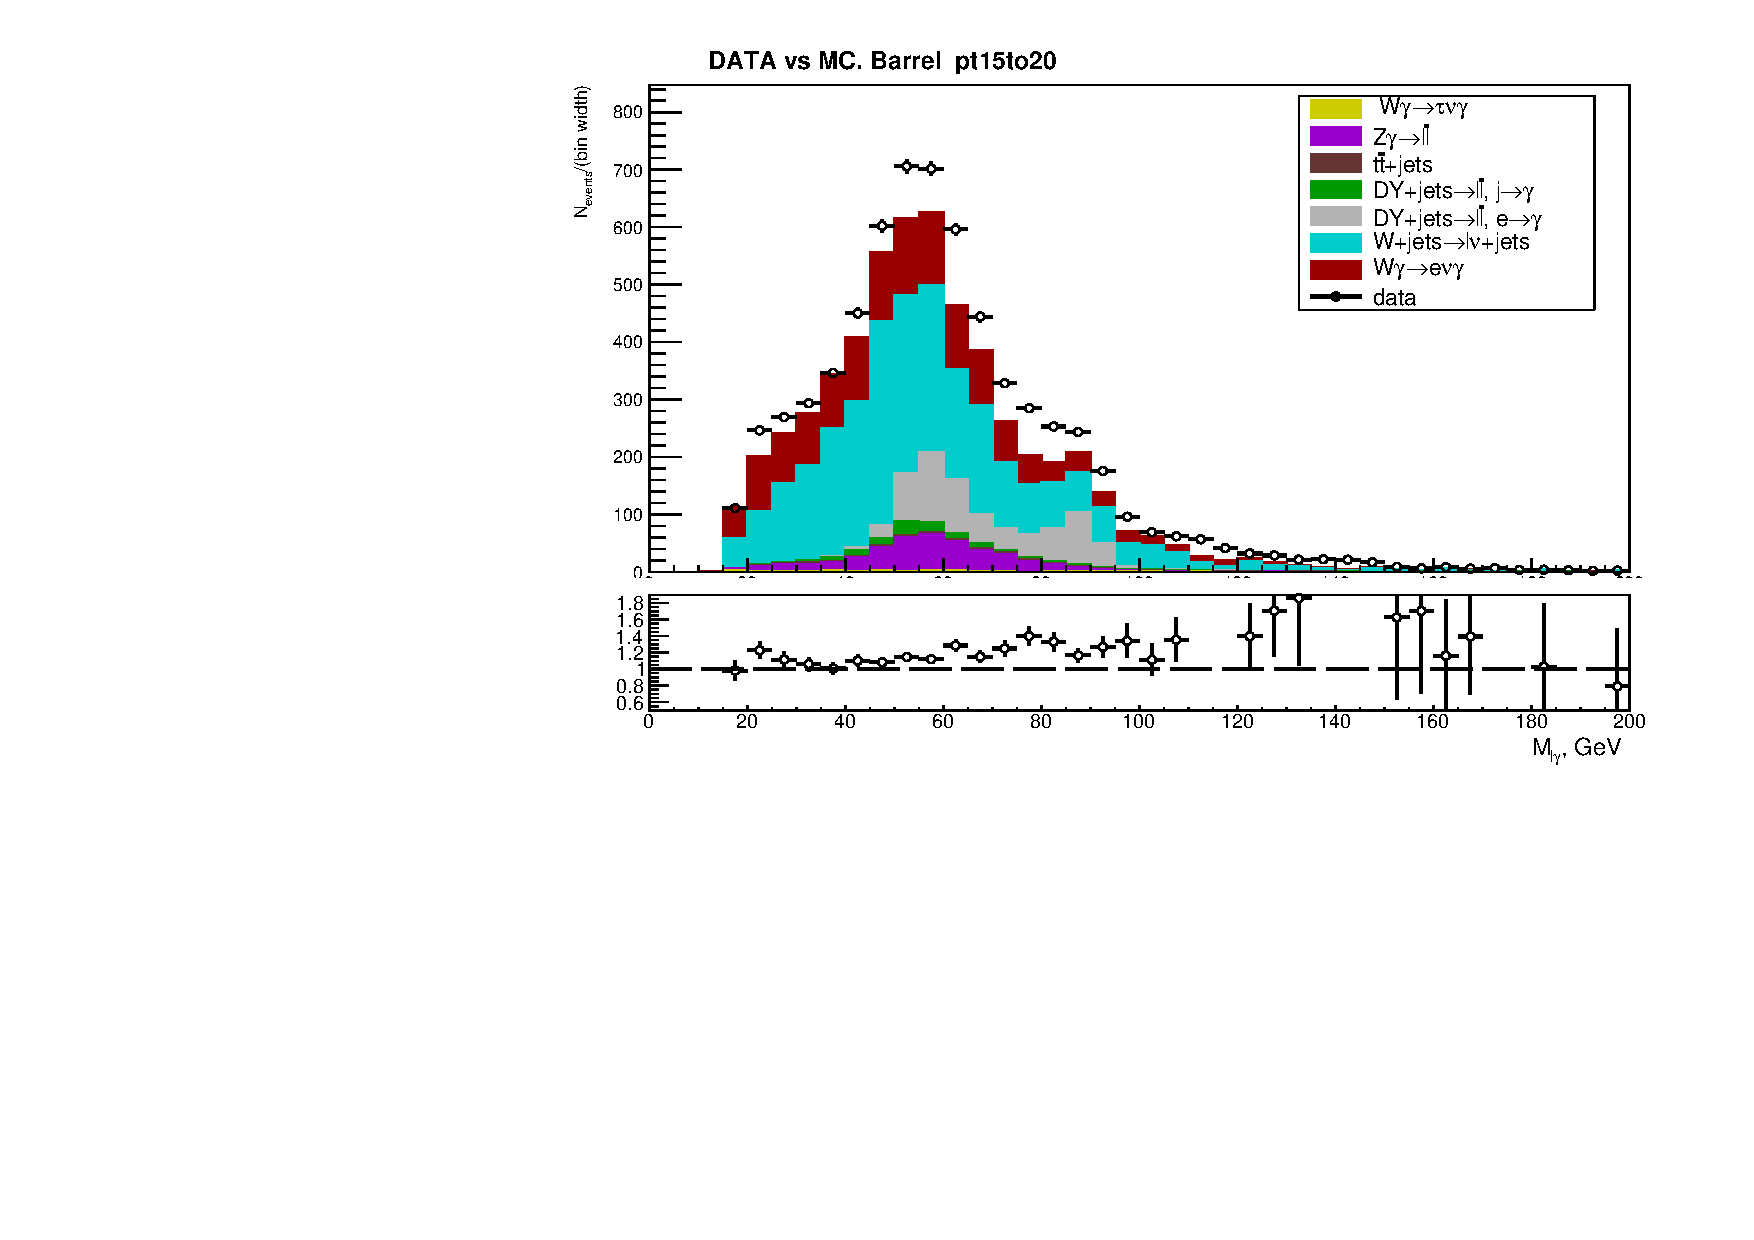
\includegraphics[width=0.40\textwidth]{../figs/figs_v11/ELECTRON_WGamma/PrepareYields/c_TotalDATAvsMC_Barrel__Mpholep1PRELIMINARY_FOR_E_TO_GAMMA_WITH_PSV_CUT_pt15to20_.pdf}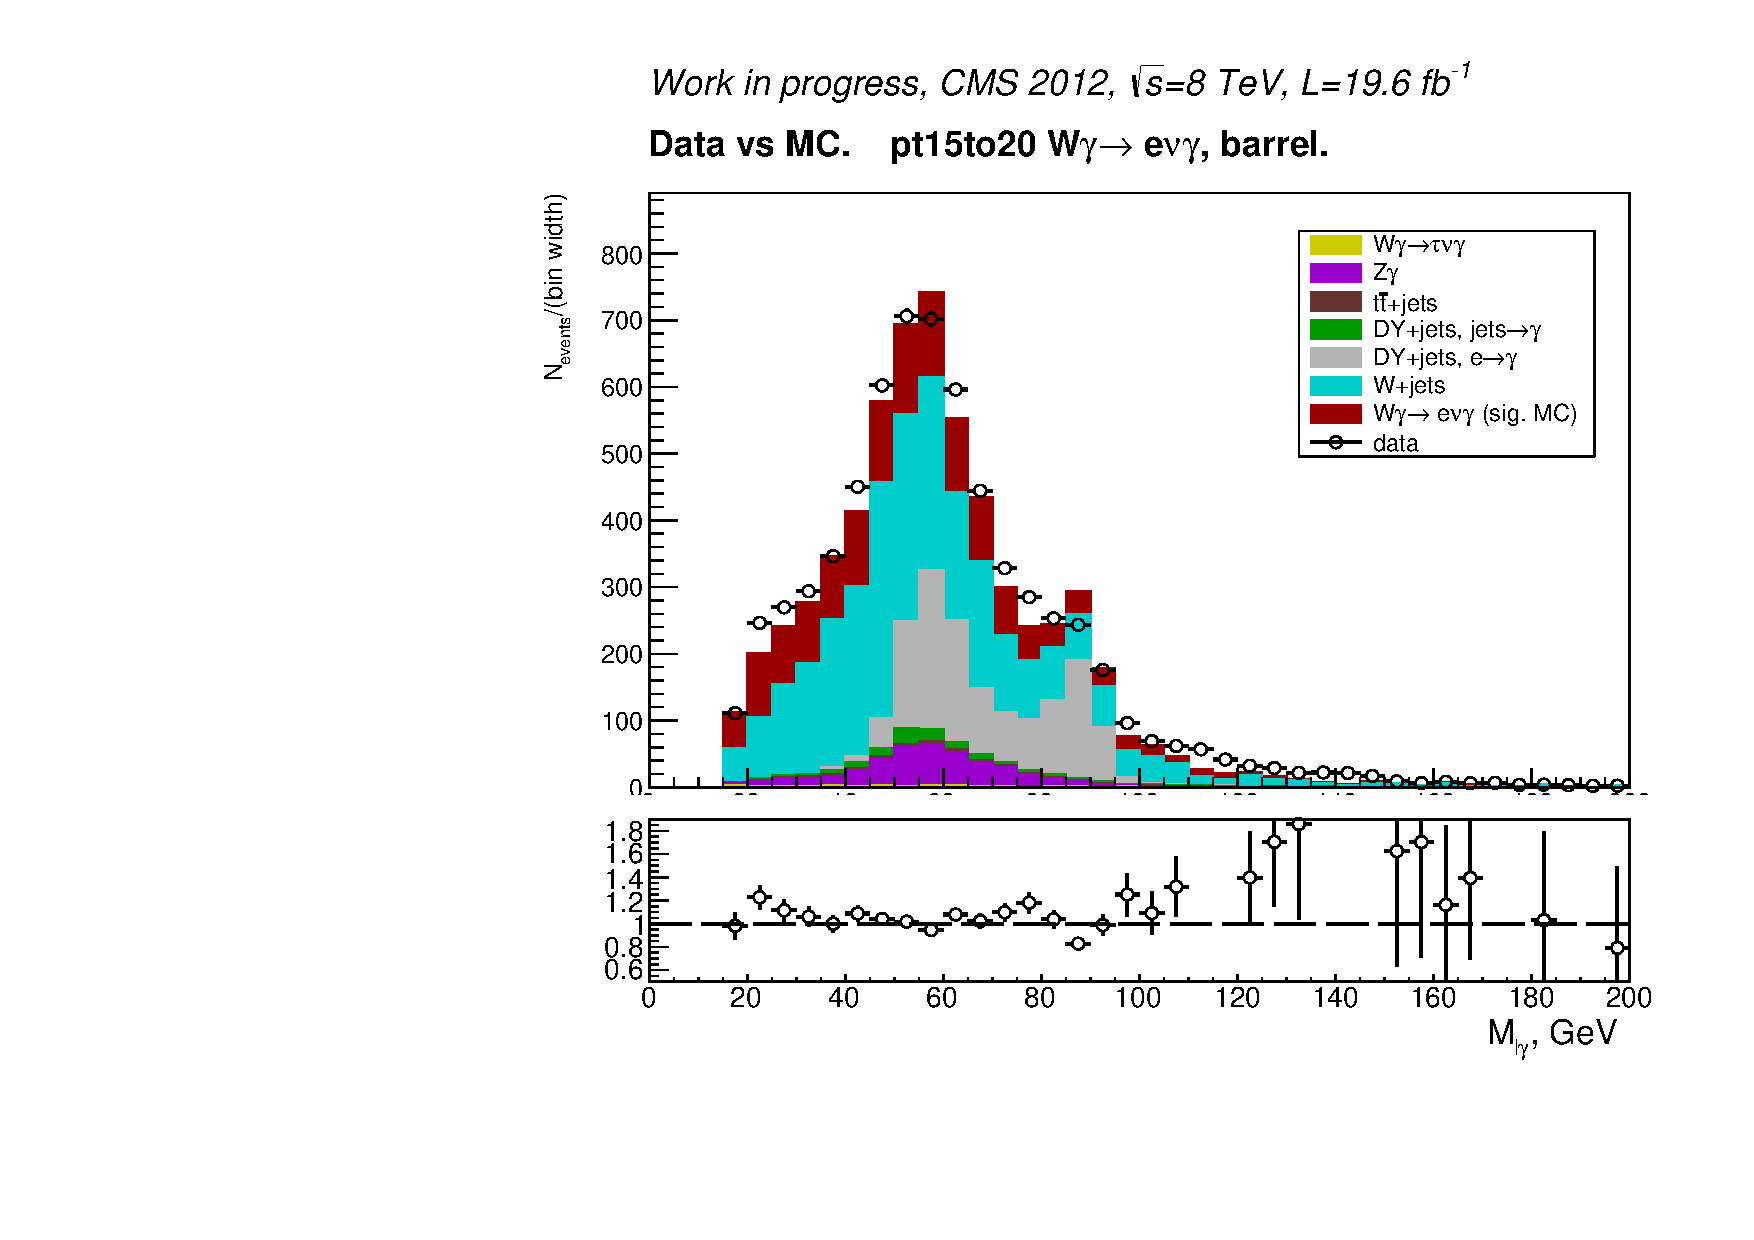
\includegraphics[width=0.40\textwidth]{../figs/figs_v11/ELECTRON_WGamma/PrepareYields/c_TotalDATAvsMC_Barrel__Mpholep1PRELIMINARY_FOR_E_TO_GAMMA_WITH_PSV_CUT_pt15to20__etogScale.pdf}\\
    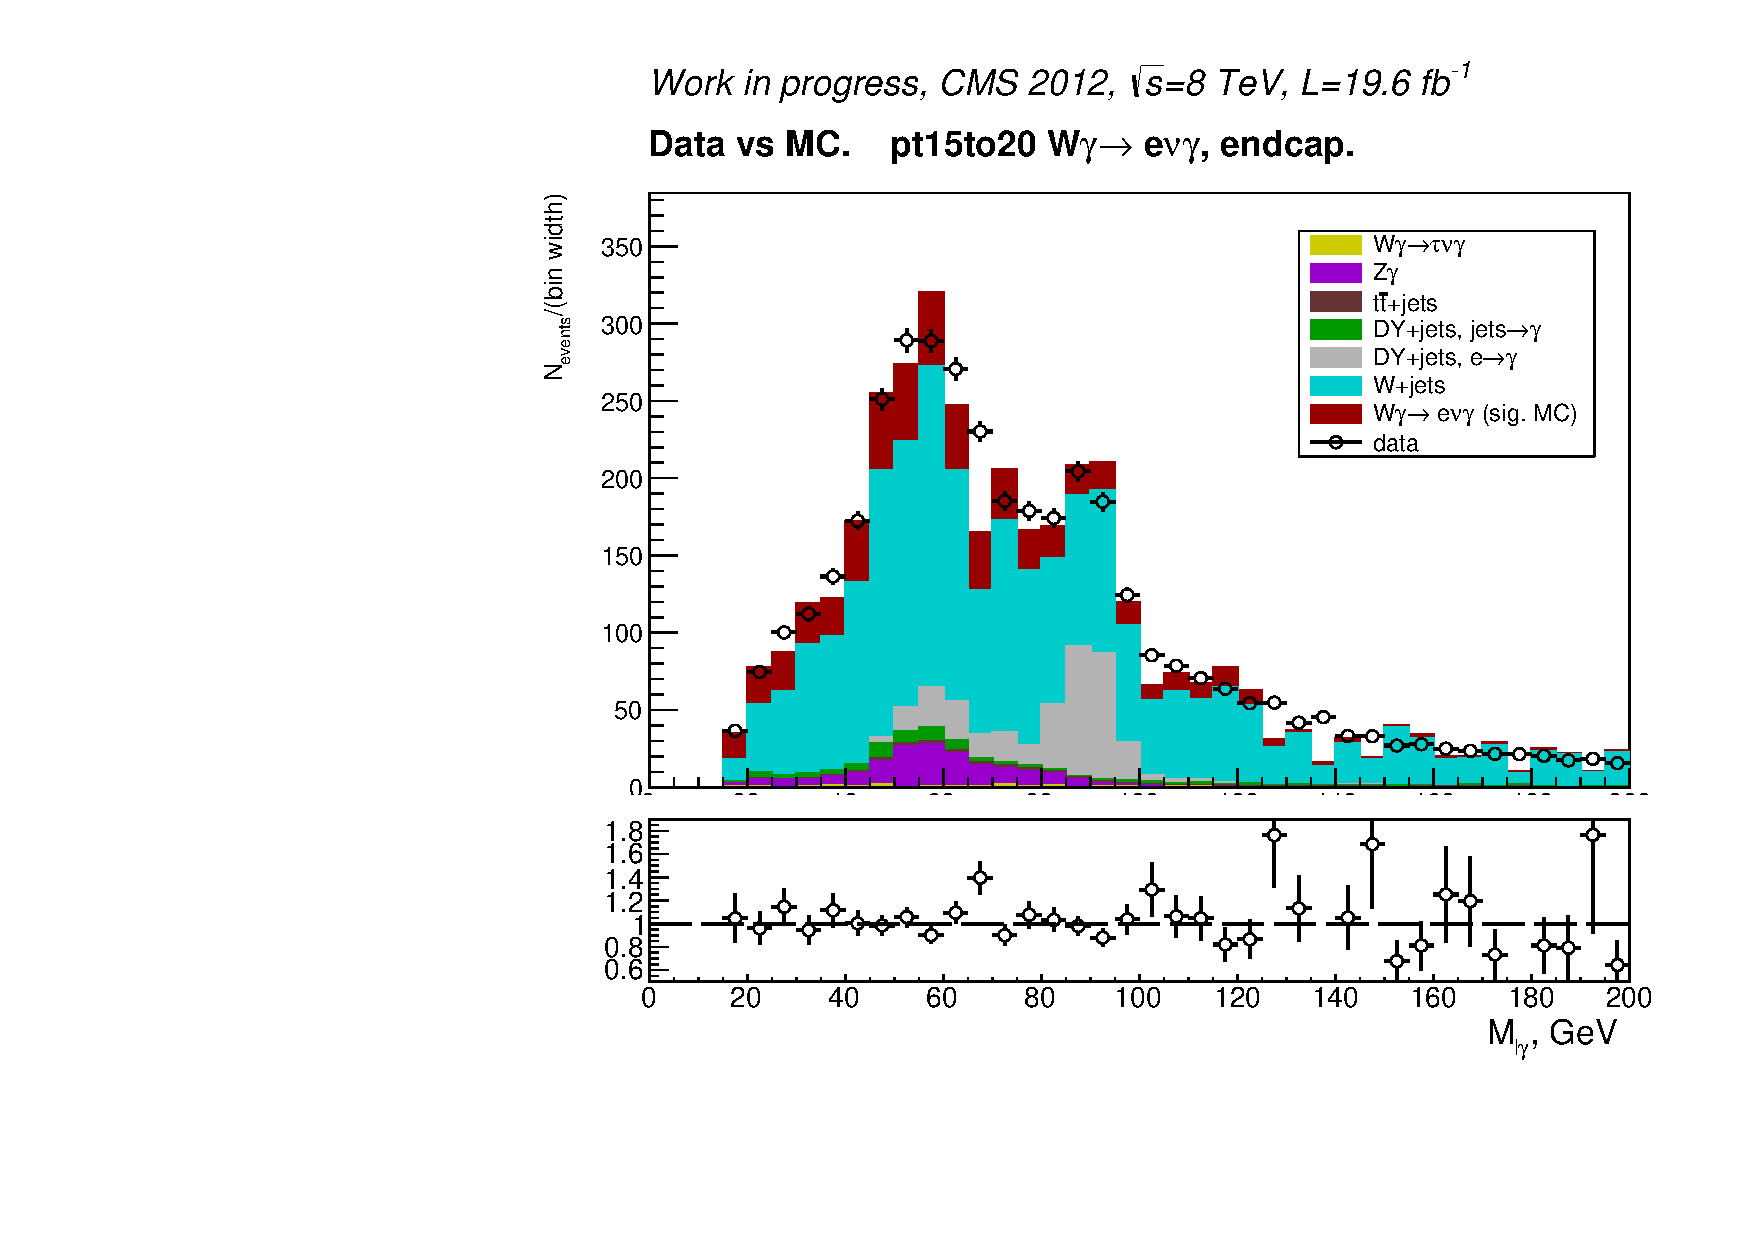
\includegraphics[width=0.40\textwidth]{../figs/figs_v11/ELECTRON_WGamma/PrepareYields/c_TotalDATAvsMC_Endcap__Mpholep1PRELIMINARY_FOR_E_TO_GAMMA_WITH_PSV_CUT_pt15to20_.pdf}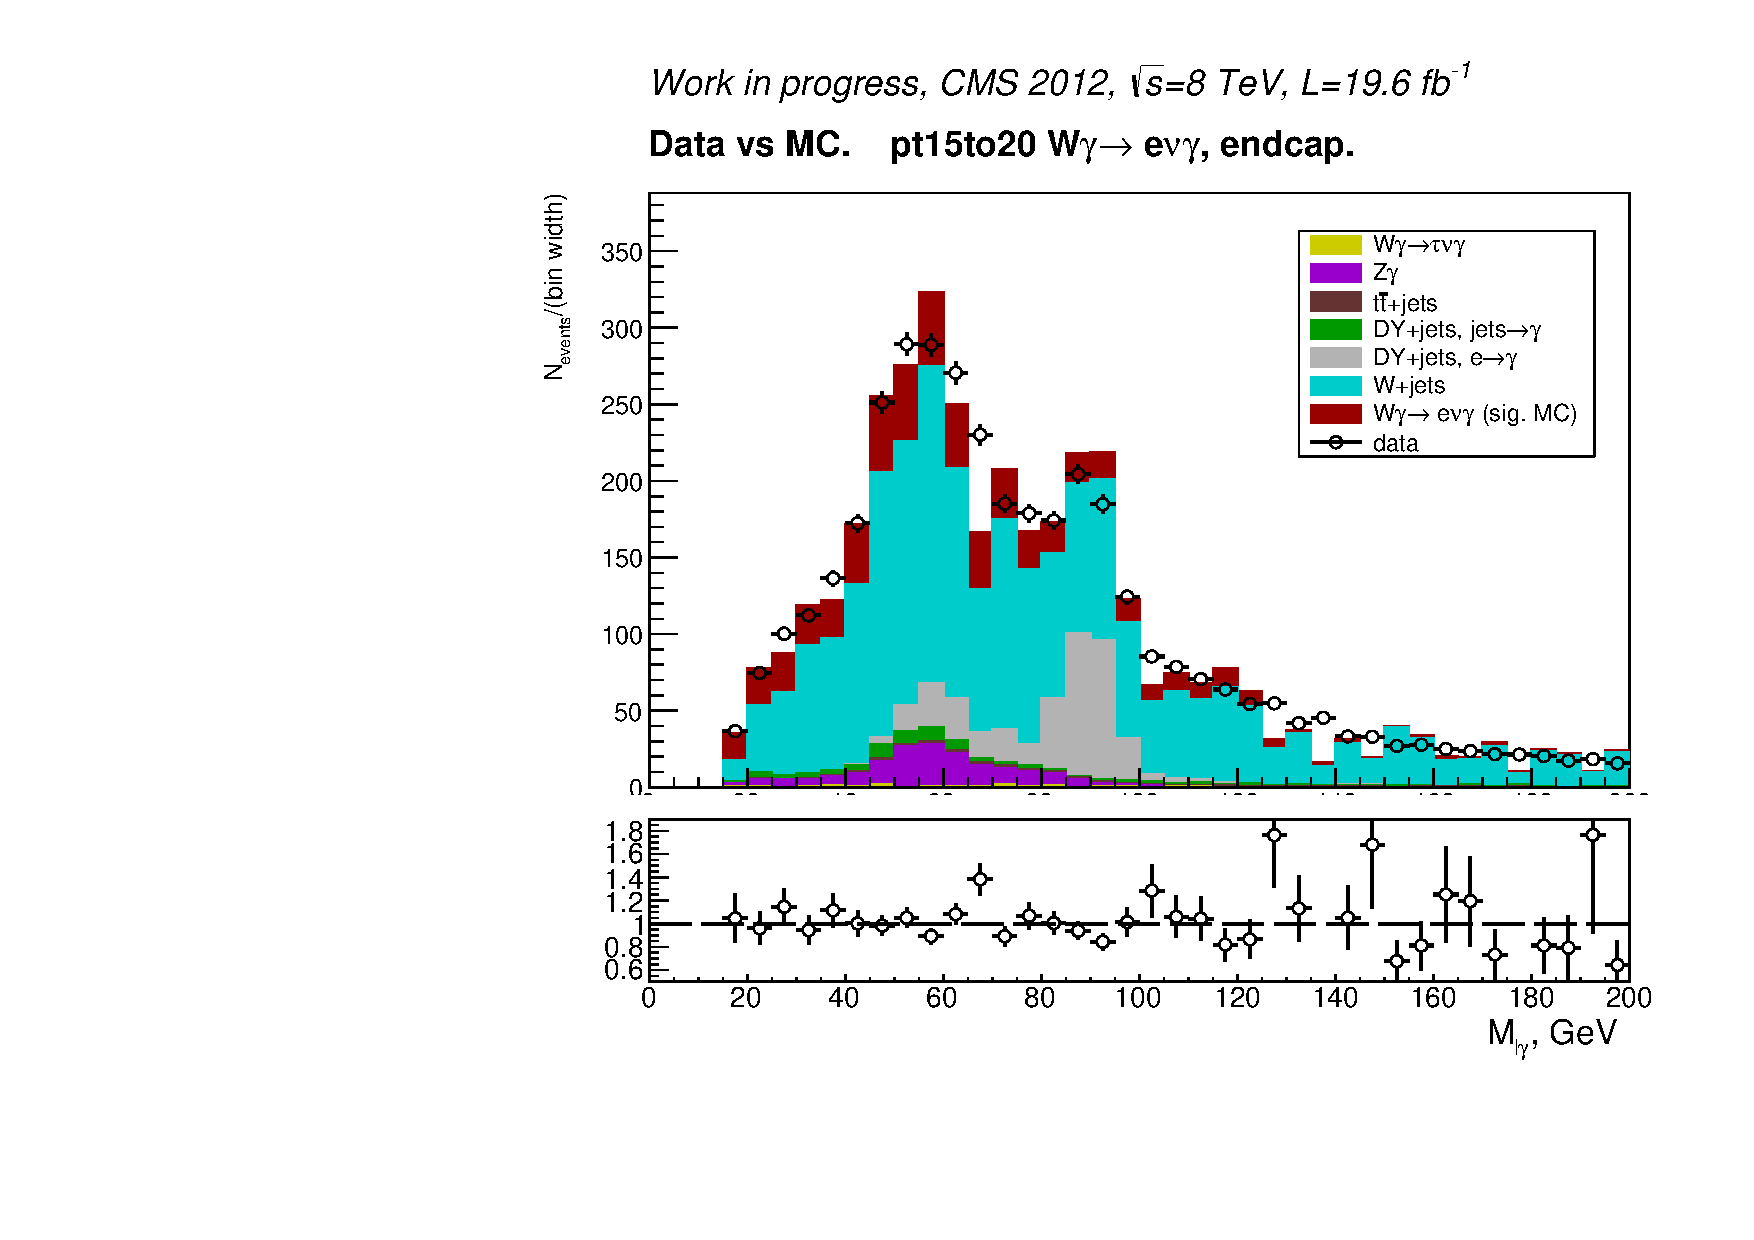
\includegraphics[width=0.40\textwidth]{../figs/figs_v11/ELECTRON_WGamma/PrepareYields/c_TotalDATAvsMC_Endcap__Mpholep1PRELIMINARY_FOR_E_TO_GAMMA_WITH_PSV_CUT_pt15to20__etogScale.pdf}\\
    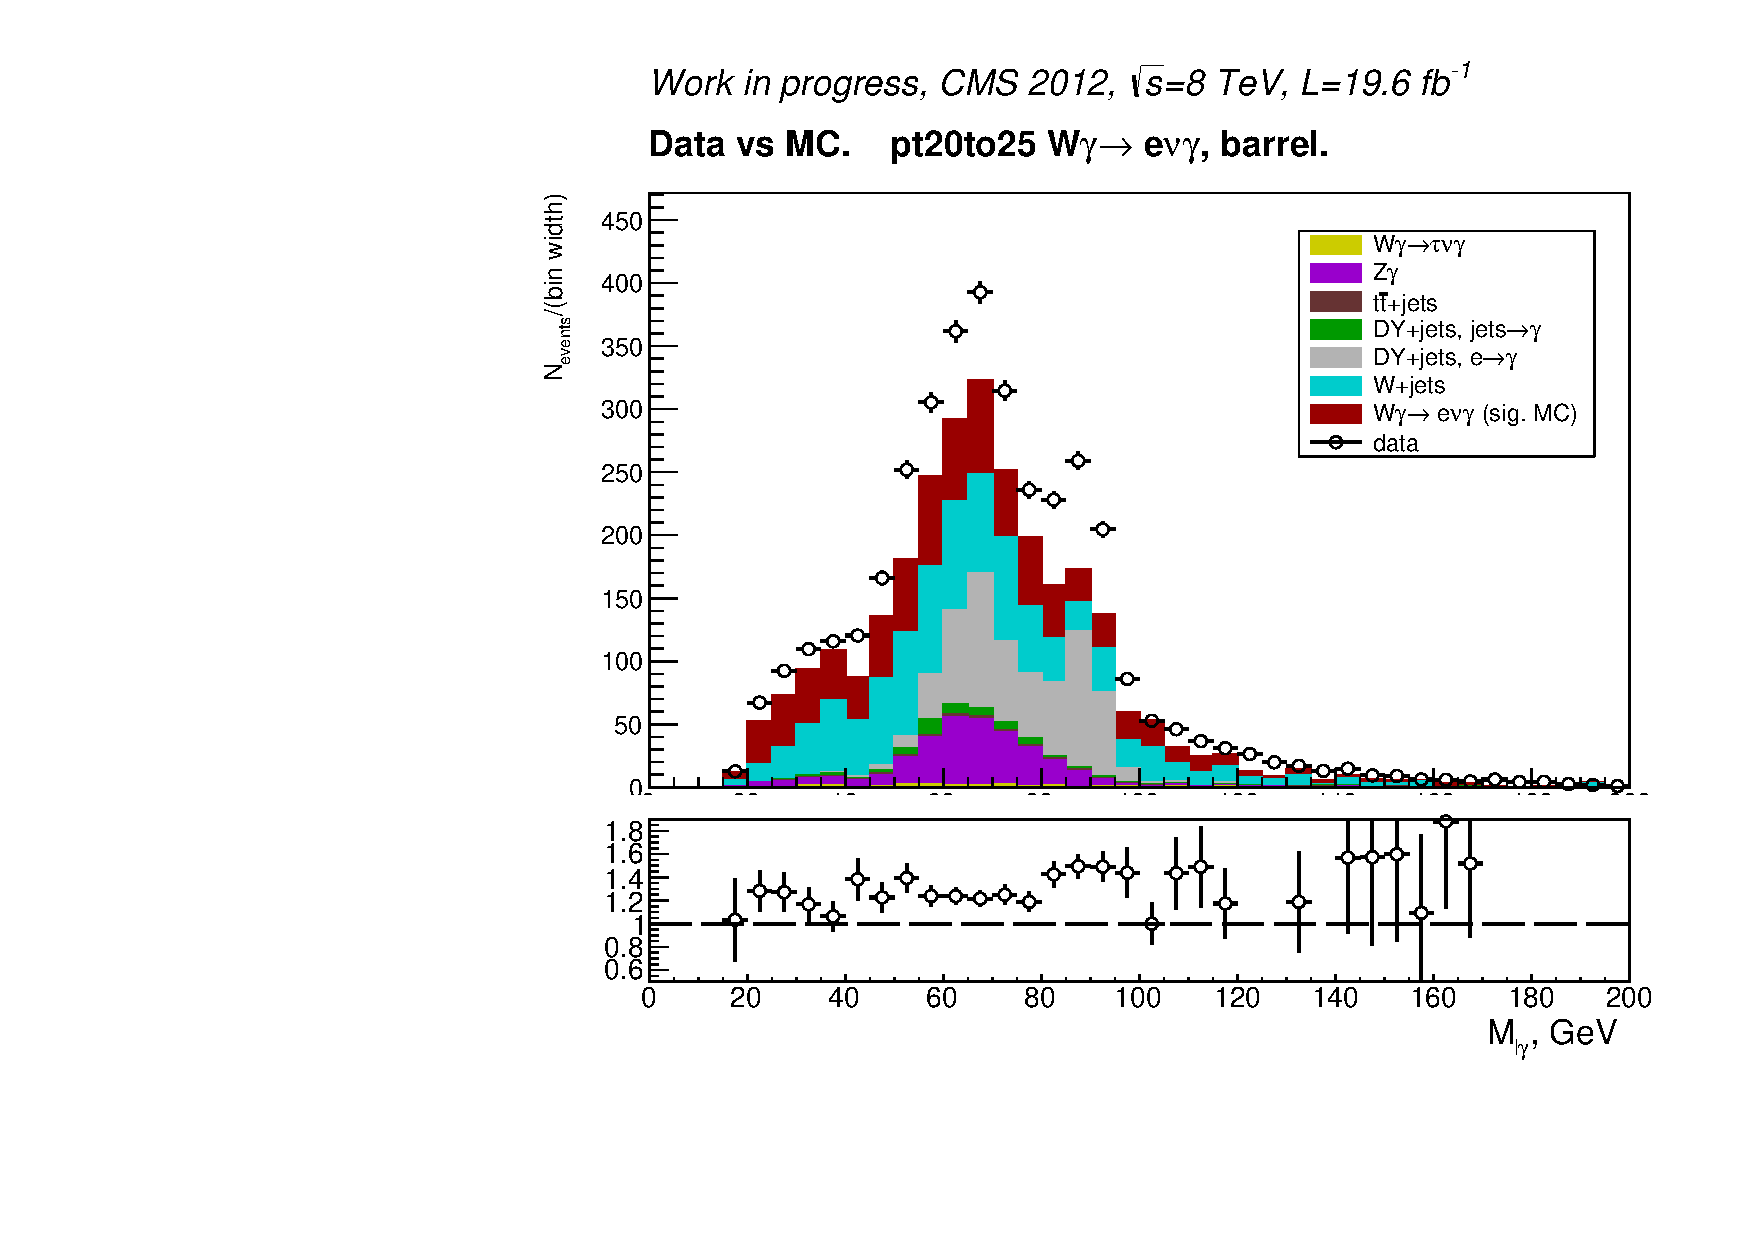
\includegraphics[width=0.40\textwidth]{../figs/figs_v11/ELECTRON_WGamma/PrepareYields/c_TotalDATAvsMC_Barrel__Mpholep1PRELIMINARY_FOR_E_TO_GAMMA_WITH_PSV_CUT_pt20to25_.pdf}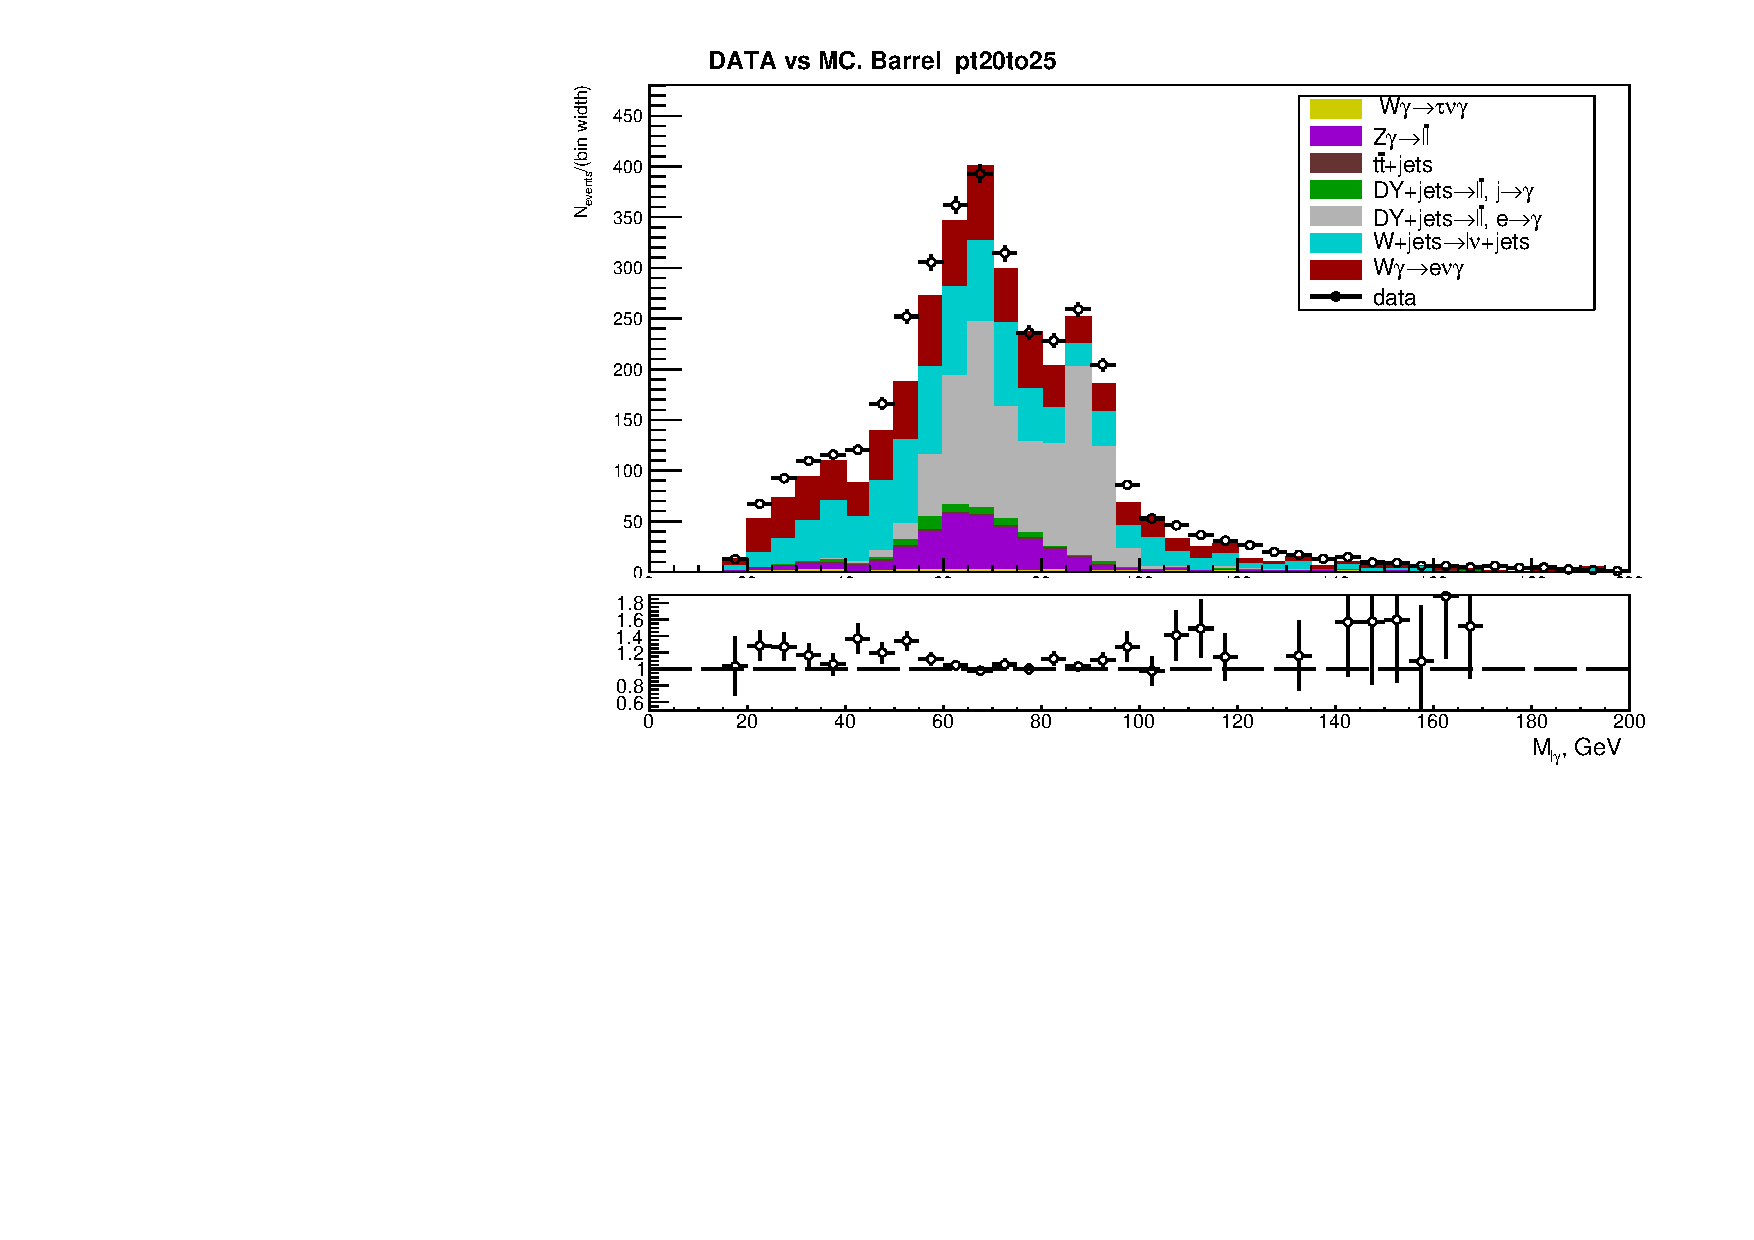
\includegraphics[width=0.40\textwidth]{../figs/figs_v11/ELECTRON_WGamma/PrepareYields/c_TotalDATAvsMC_Barrel__Mpholep1PRELIMINARY_FOR_E_TO_GAMMA_WITH_PSV_CUT_pt20to25__etogScale.pdf}\\
    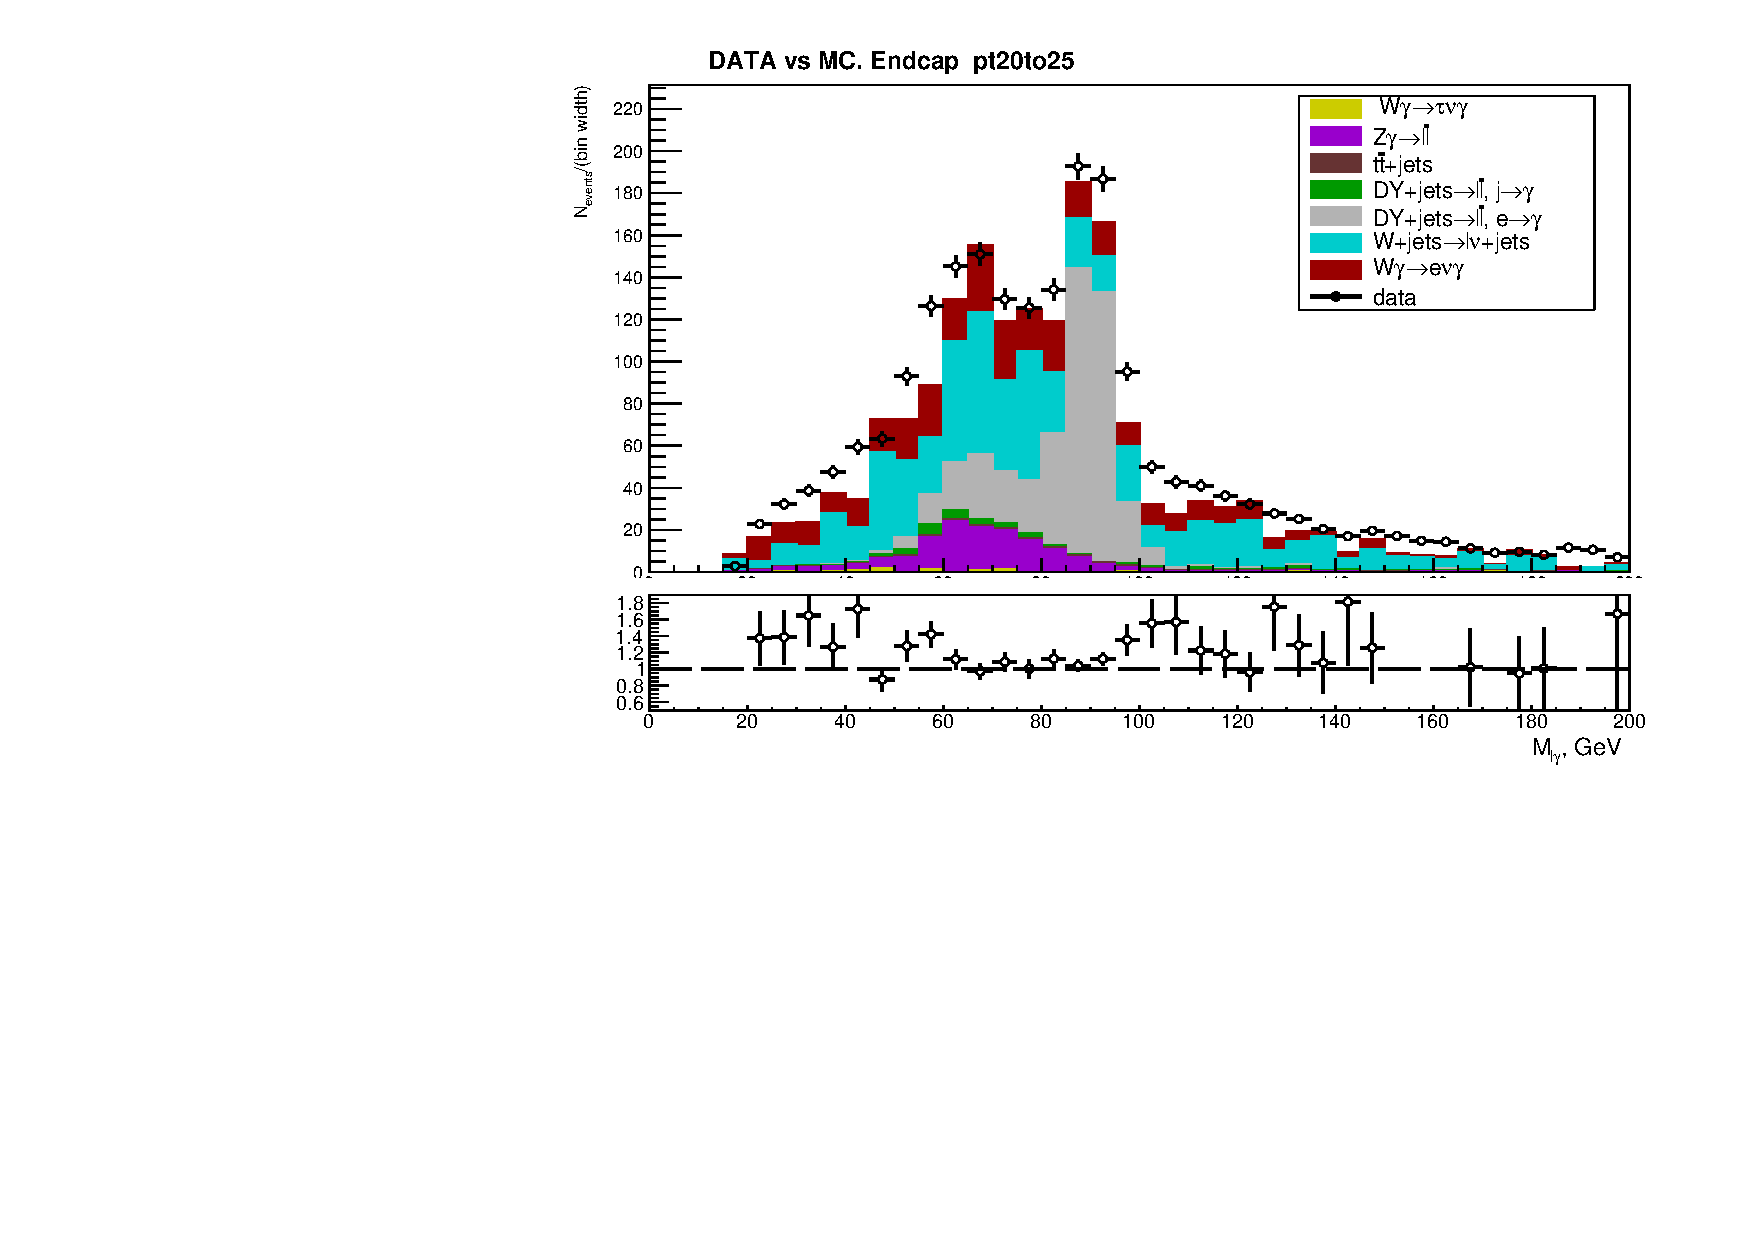
\includegraphics[width=0.40\textwidth]{../figs/figs_v11/ELECTRON_WGamma/PrepareYields/c_TotalDATAvsMC_Endcap__Mpholep1PRELIMINARY_FOR_E_TO_GAMMA_WITH_PSV_CUT_pt20to25_.pdf} 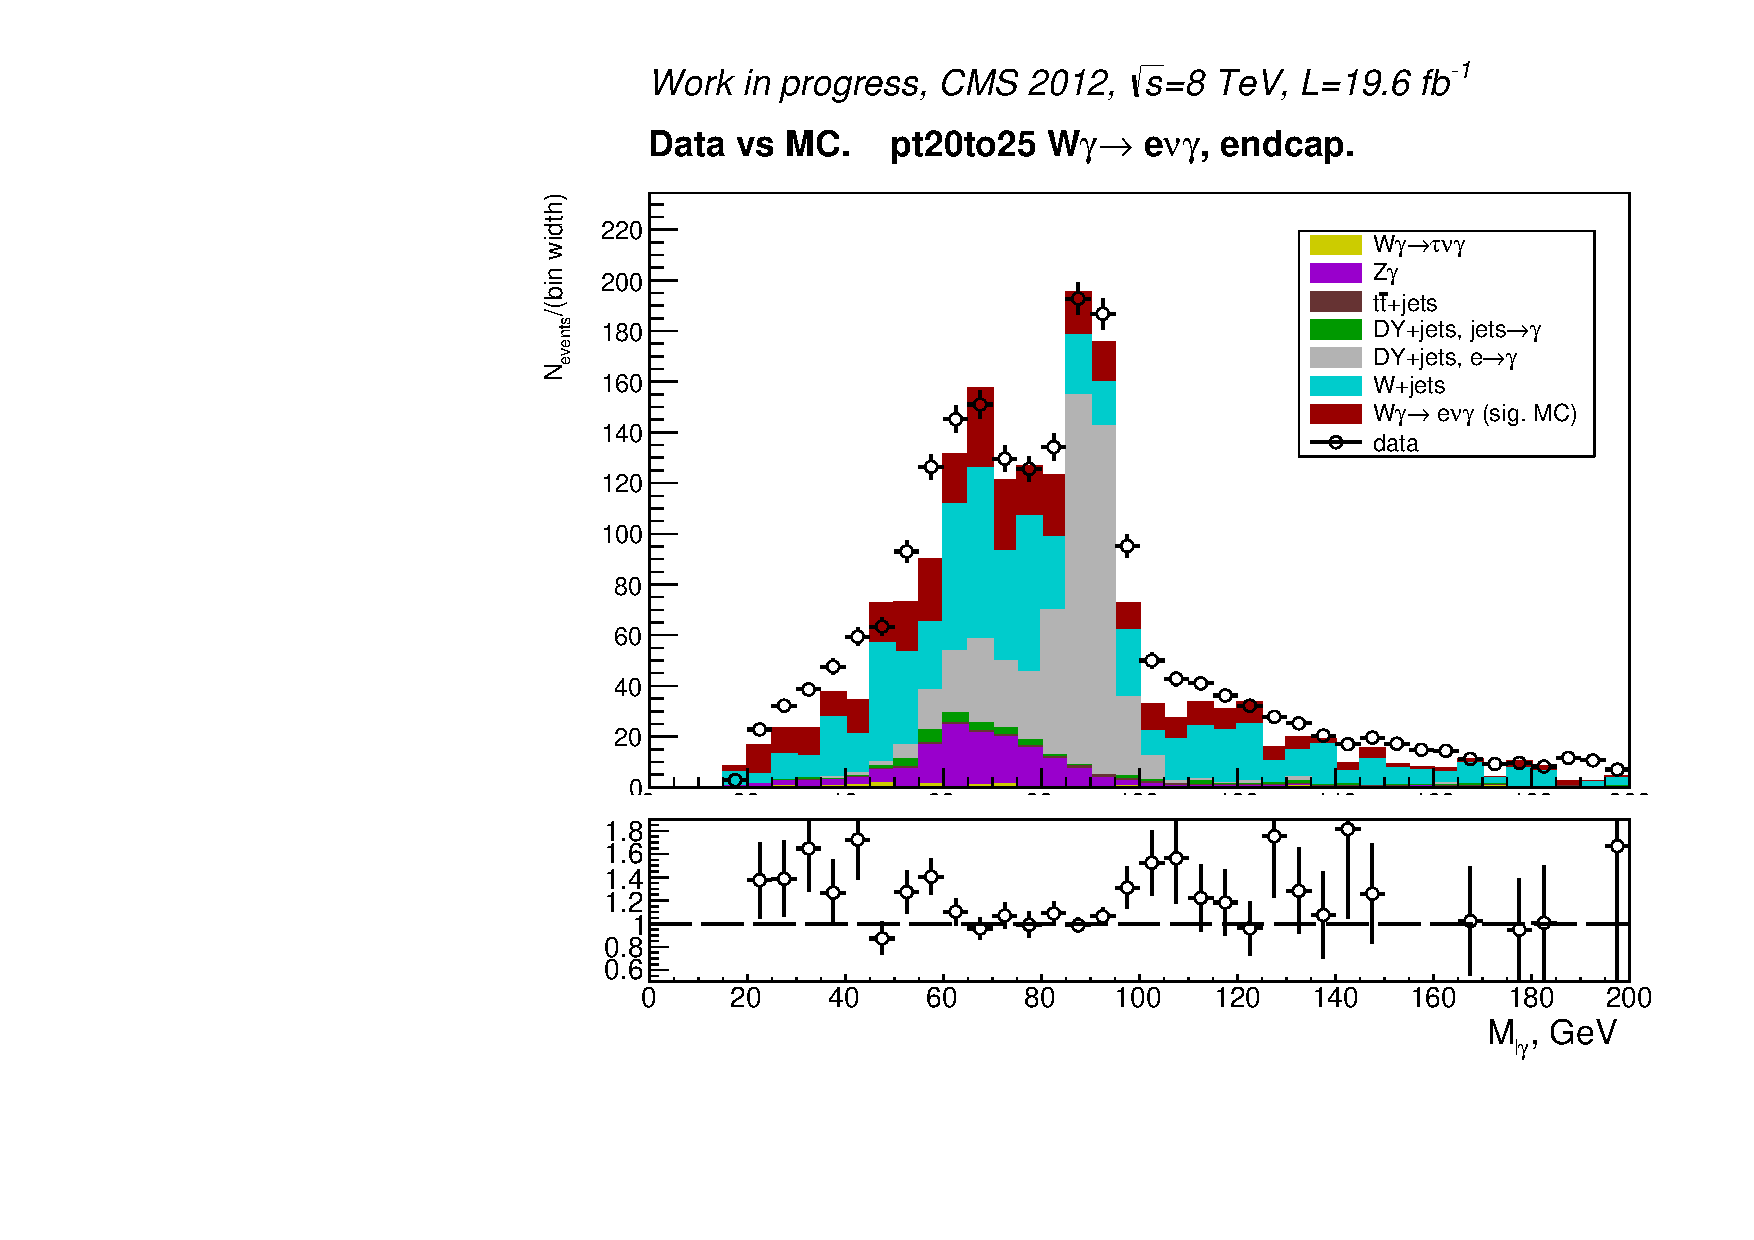
\includegraphics[width=0.40\textwidth]{../figs/figs_v11/ELECTRON_WGamma/PrepareYields/c_TotalDATAvsMC_Endcap__Mpholep1PRELIMINARY_FOR_E_TO_GAMMA_WITH_PSV_CUT_pt20to25__etogScale.pdf}\\
   \label{fig:Mpholep1DatavsMC_15to25}
  \caption{$M_{e,\gamma}$ distribution, data vs MC. Bins 15-20-25 GeV. Left: all MC samples are normalized to luminocity of data, PU weight adn SFs, right: DY$\rightarrow$jets(e$\rightarrow\gamma$) also normalized to e$\rightarrow\gamma$ data-driven estimates.}
  \end{center}
\end{figure}
\begin{figure}[htb]
  \begin{center}
    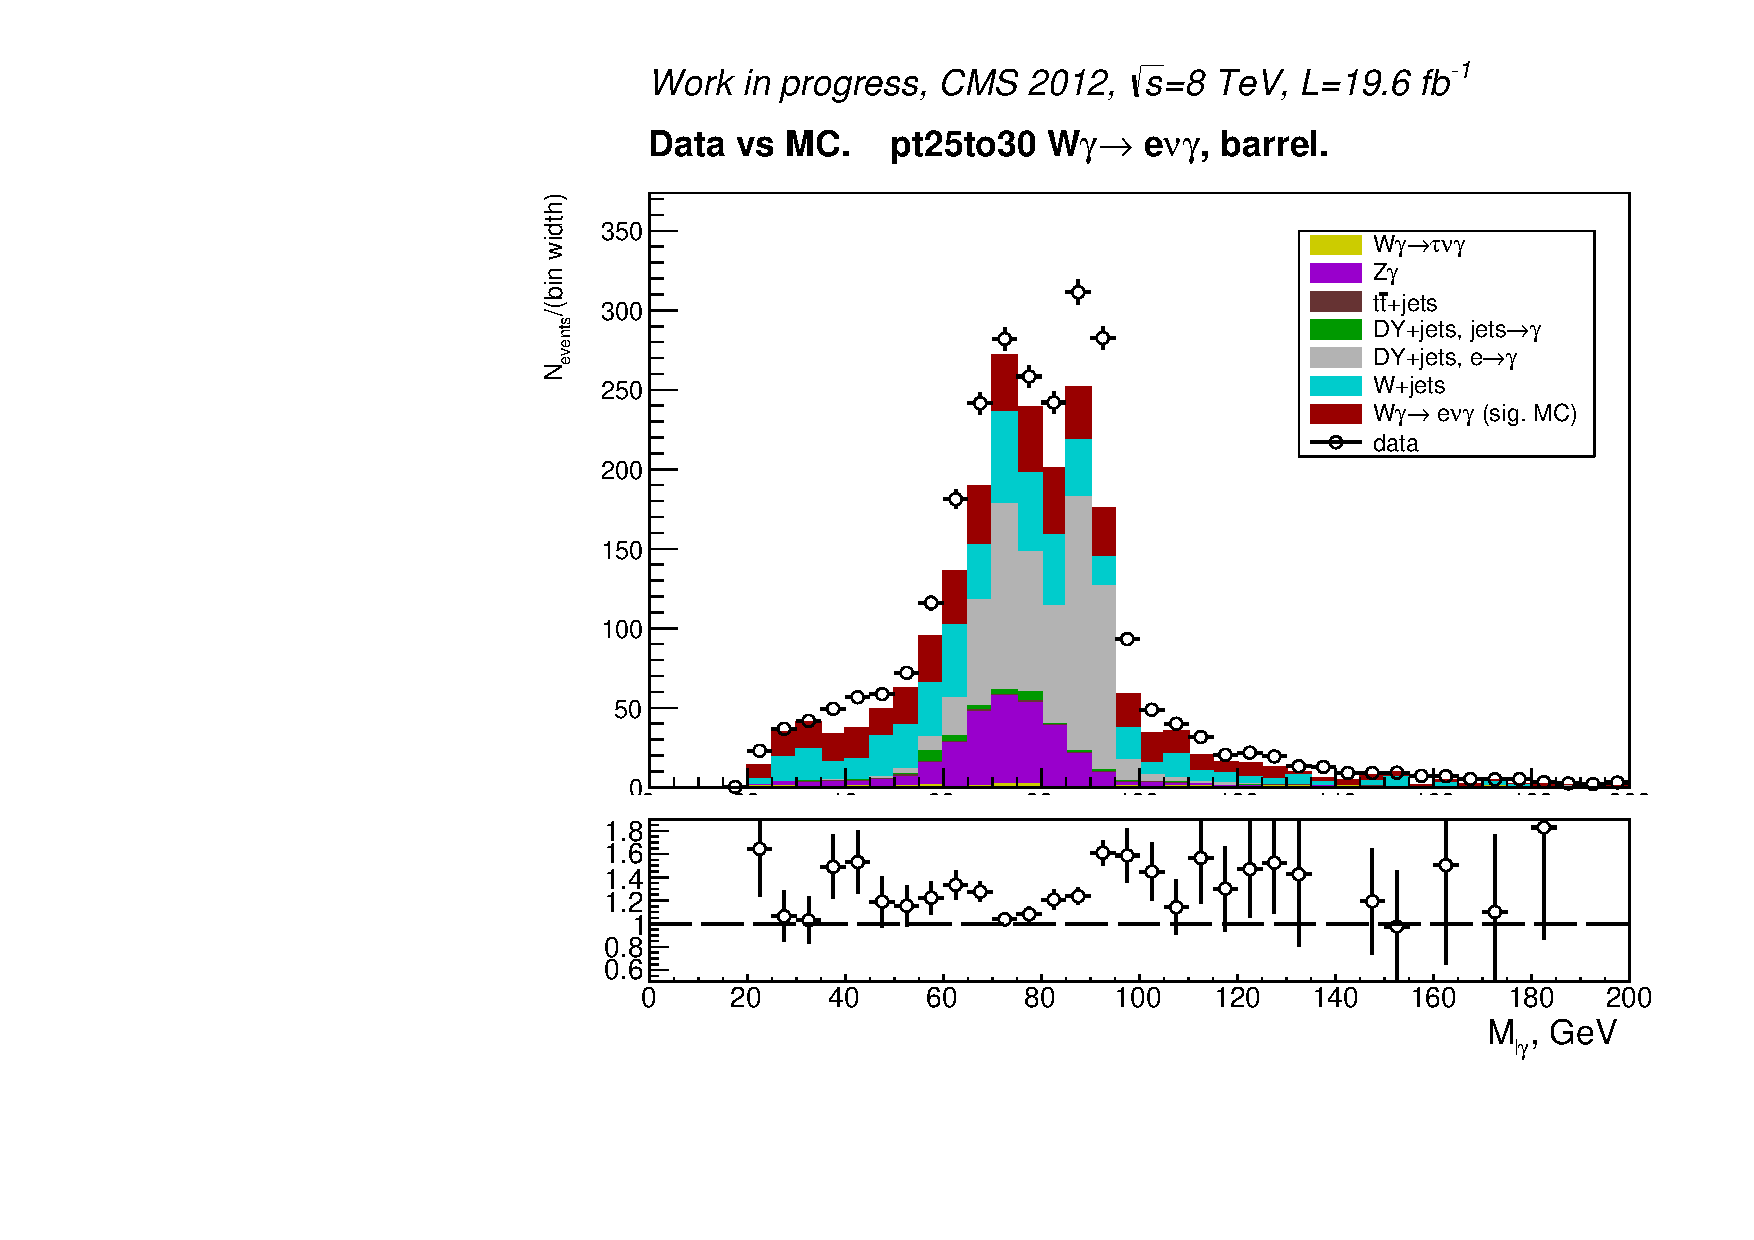
\includegraphics[width=0.40\textwidth]{../figs/figs_v11/ELECTRON_WGamma/PrepareYields/c_TotalDATAvsMC_Barrel__Mpholep1PRELIMINARY_FOR_E_TO_GAMMA_WITH_PSV_CUT_pt25to30_.pdf}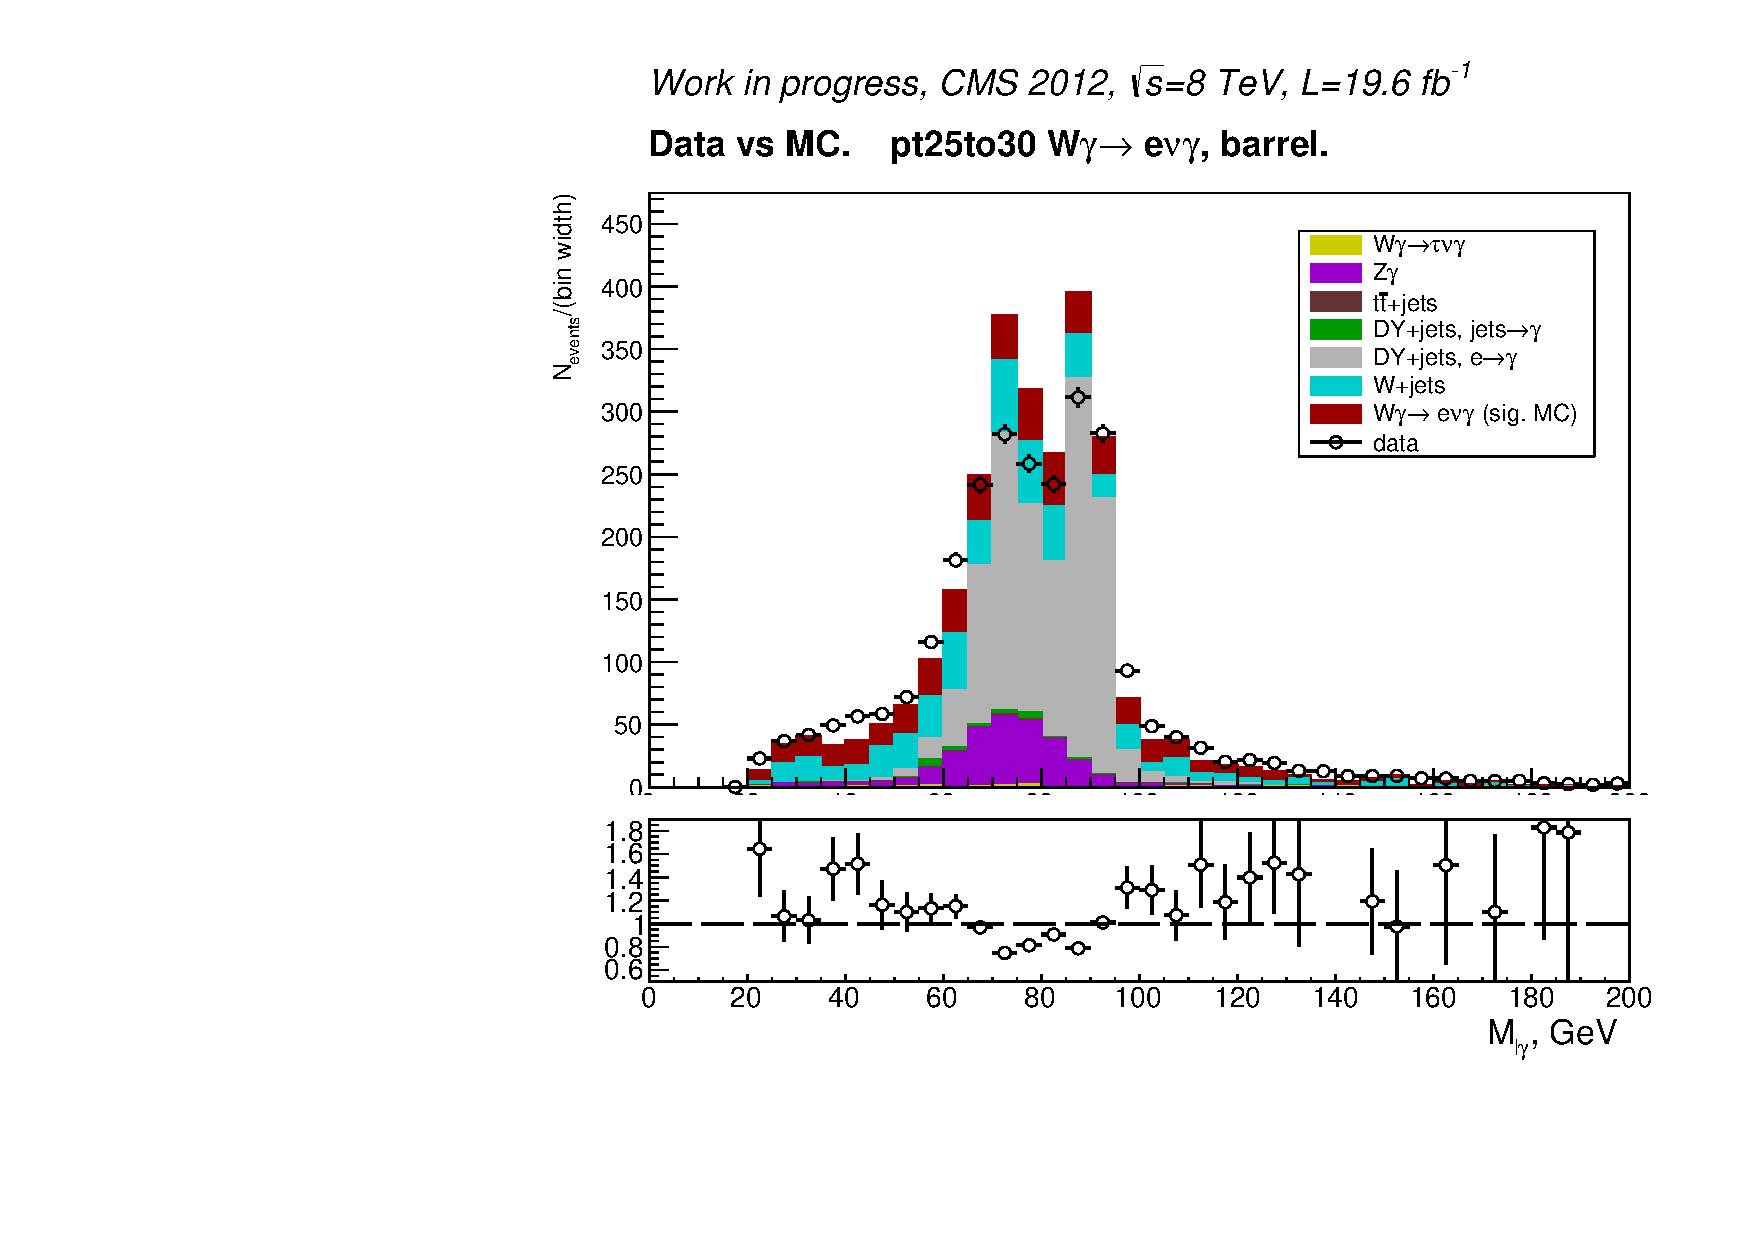
\includegraphics[width=0.40\textwidth]{../figs/figs_v11/ELECTRON_WGamma/PrepareYields/c_TotalDATAvsMC_Barrel__Mpholep1PRELIMINARY_FOR_E_TO_GAMMA_WITH_PSV_CUT_pt25to30__etogScale.pdf}   \\ 
    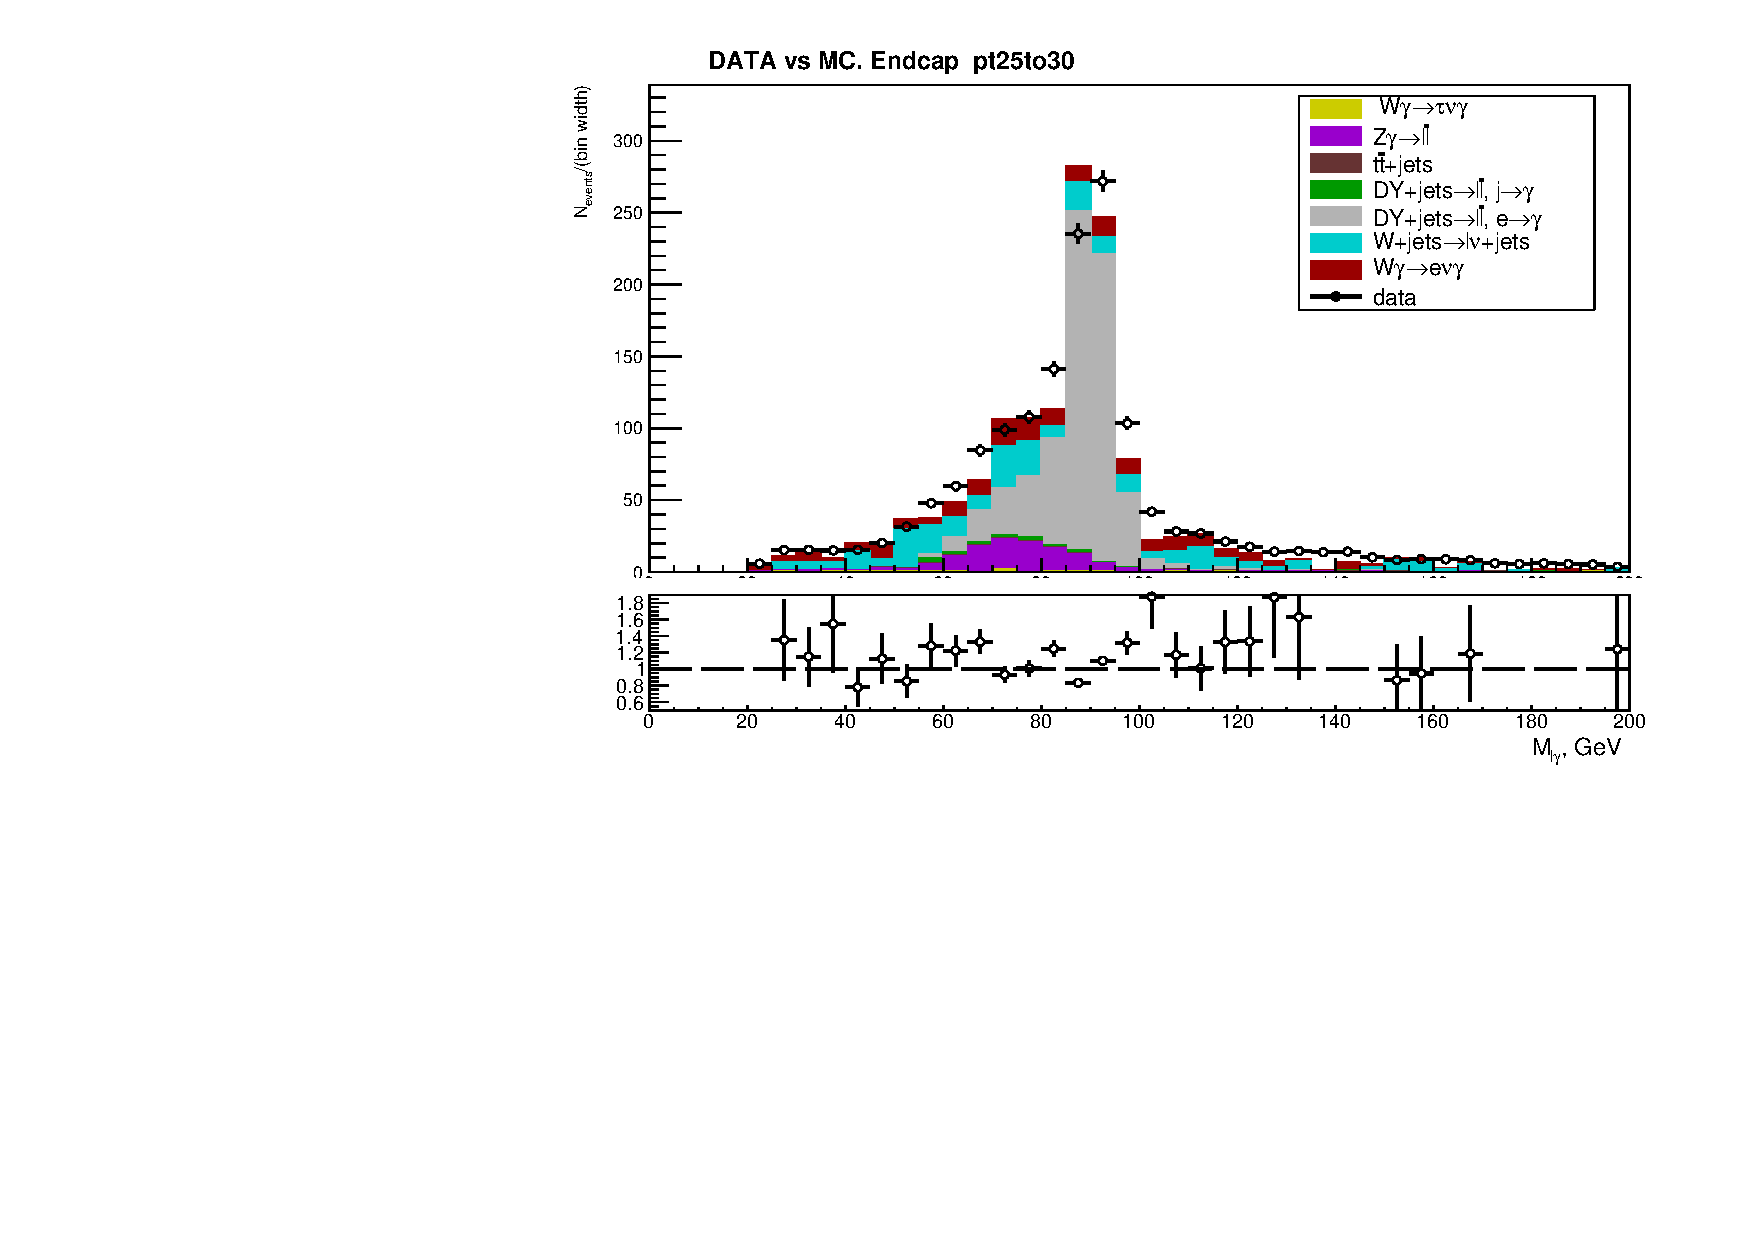
\includegraphics[width=0.40\textwidth]{../figs/figs_v11/ELECTRON_WGamma/PrepareYields/c_TotalDATAvsMC_Endcap__Mpholep1PRELIMINARY_FOR_E_TO_GAMMA_WITH_PSV_CUT_pt25to30_.pdf}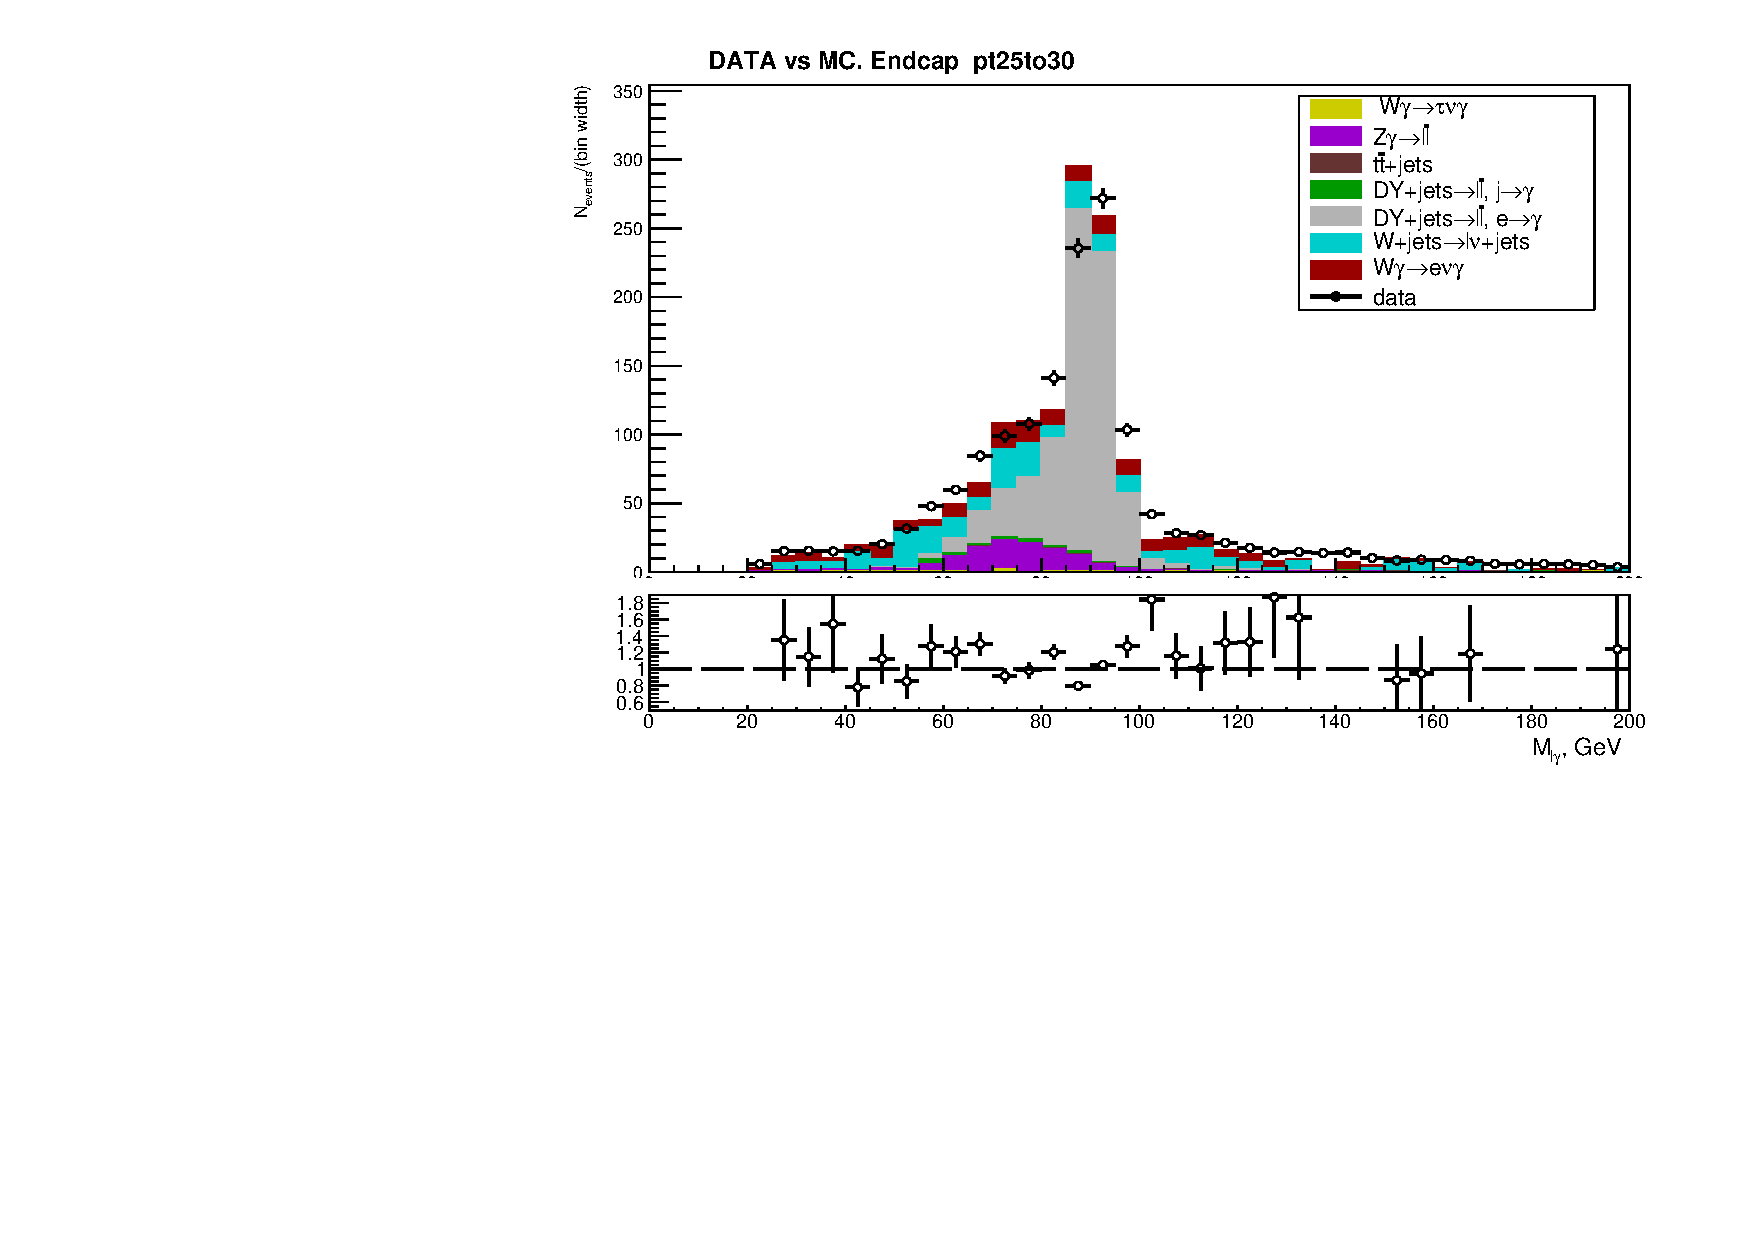
\includegraphics[width=0.40\textwidth]{../figs/figs_v11/ELECTRON_WGamma/PrepareYields/c_TotalDATAvsMC_Endcap__Mpholep1PRELIMINARY_FOR_E_TO_GAMMA_WITH_PSV_CUT_pt25to30__etogScale.pdf}\\
    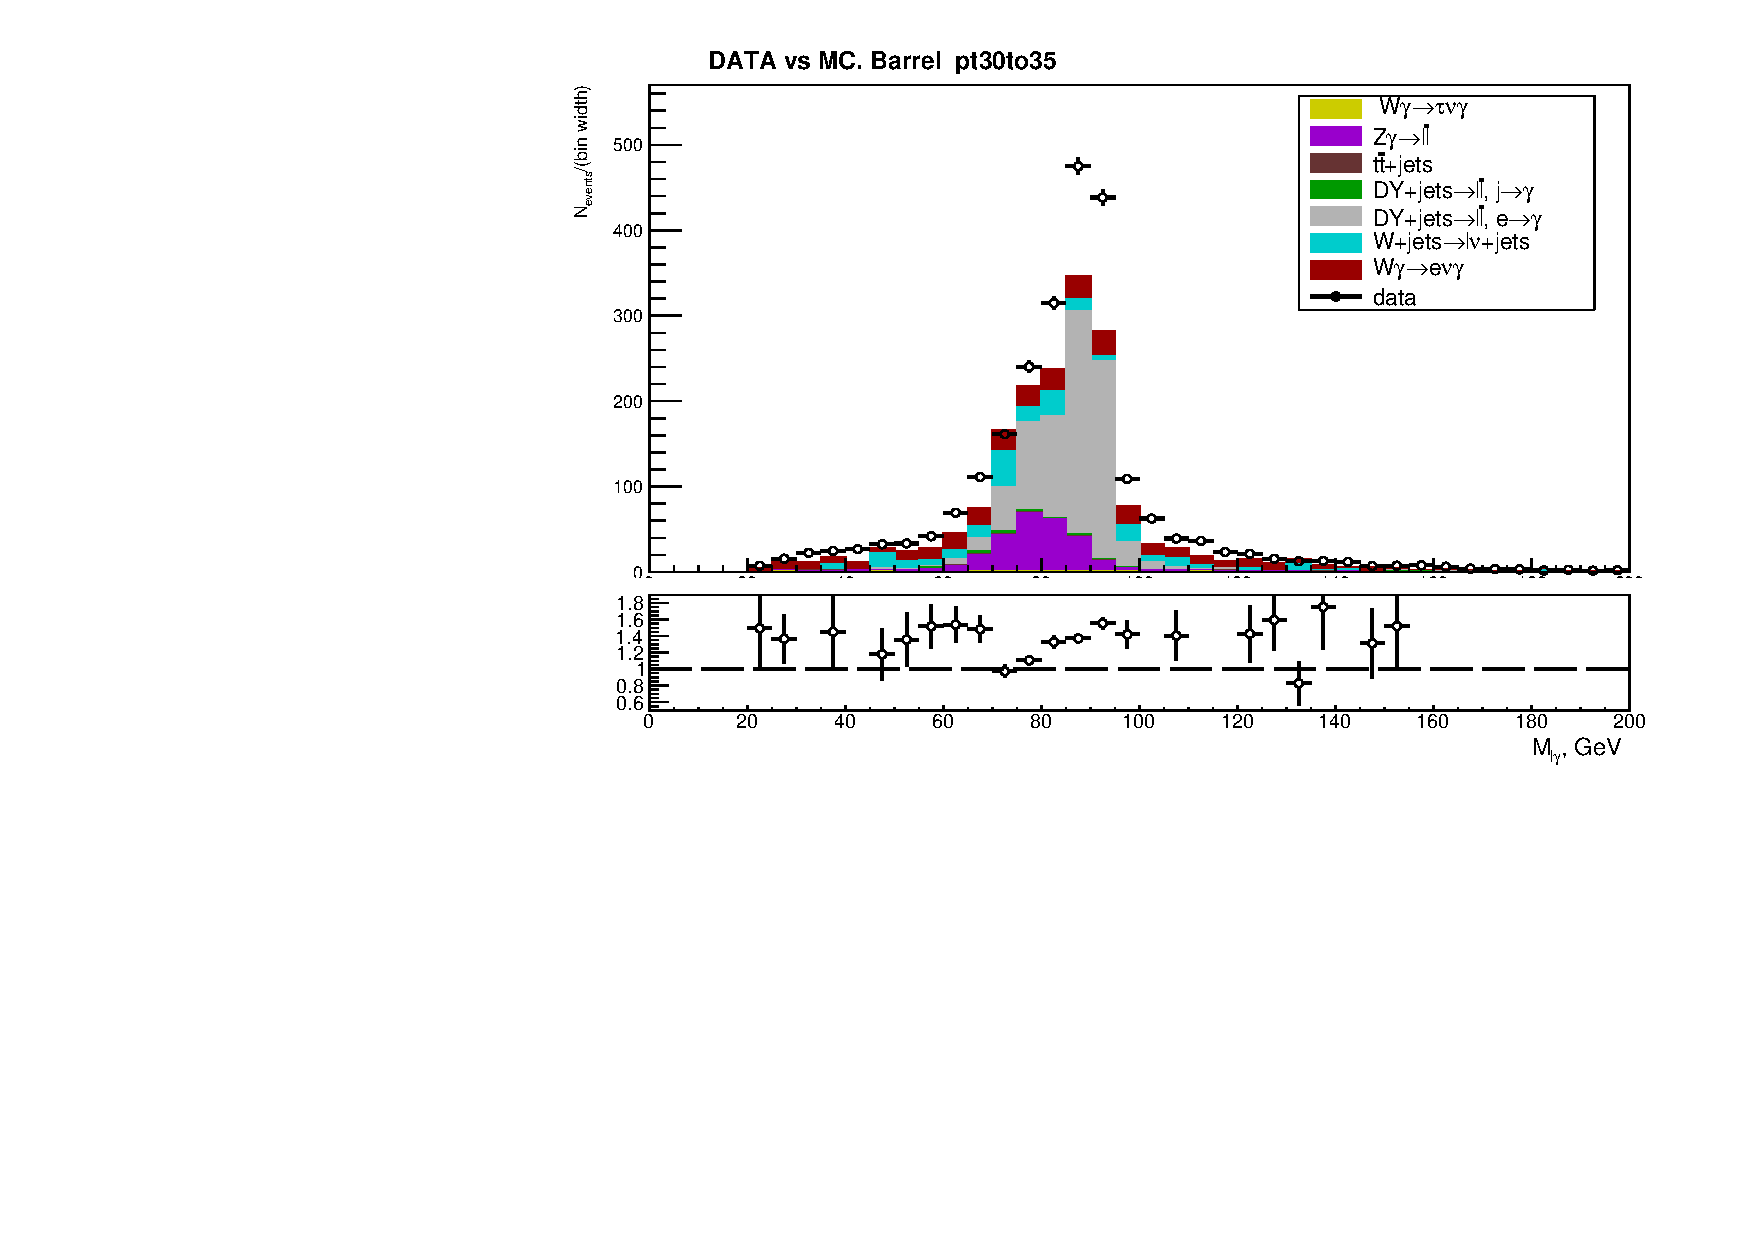
\includegraphics[width=0.40\textwidth]{../figs/figs_v11/ELECTRON_WGamma/PrepareYields/c_TotalDATAvsMC_Barrel__Mpholep1PRELIMINARY_FOR_E_TO_GAMMA_WITH_PSV_CUT_pt30to35_.pdf} 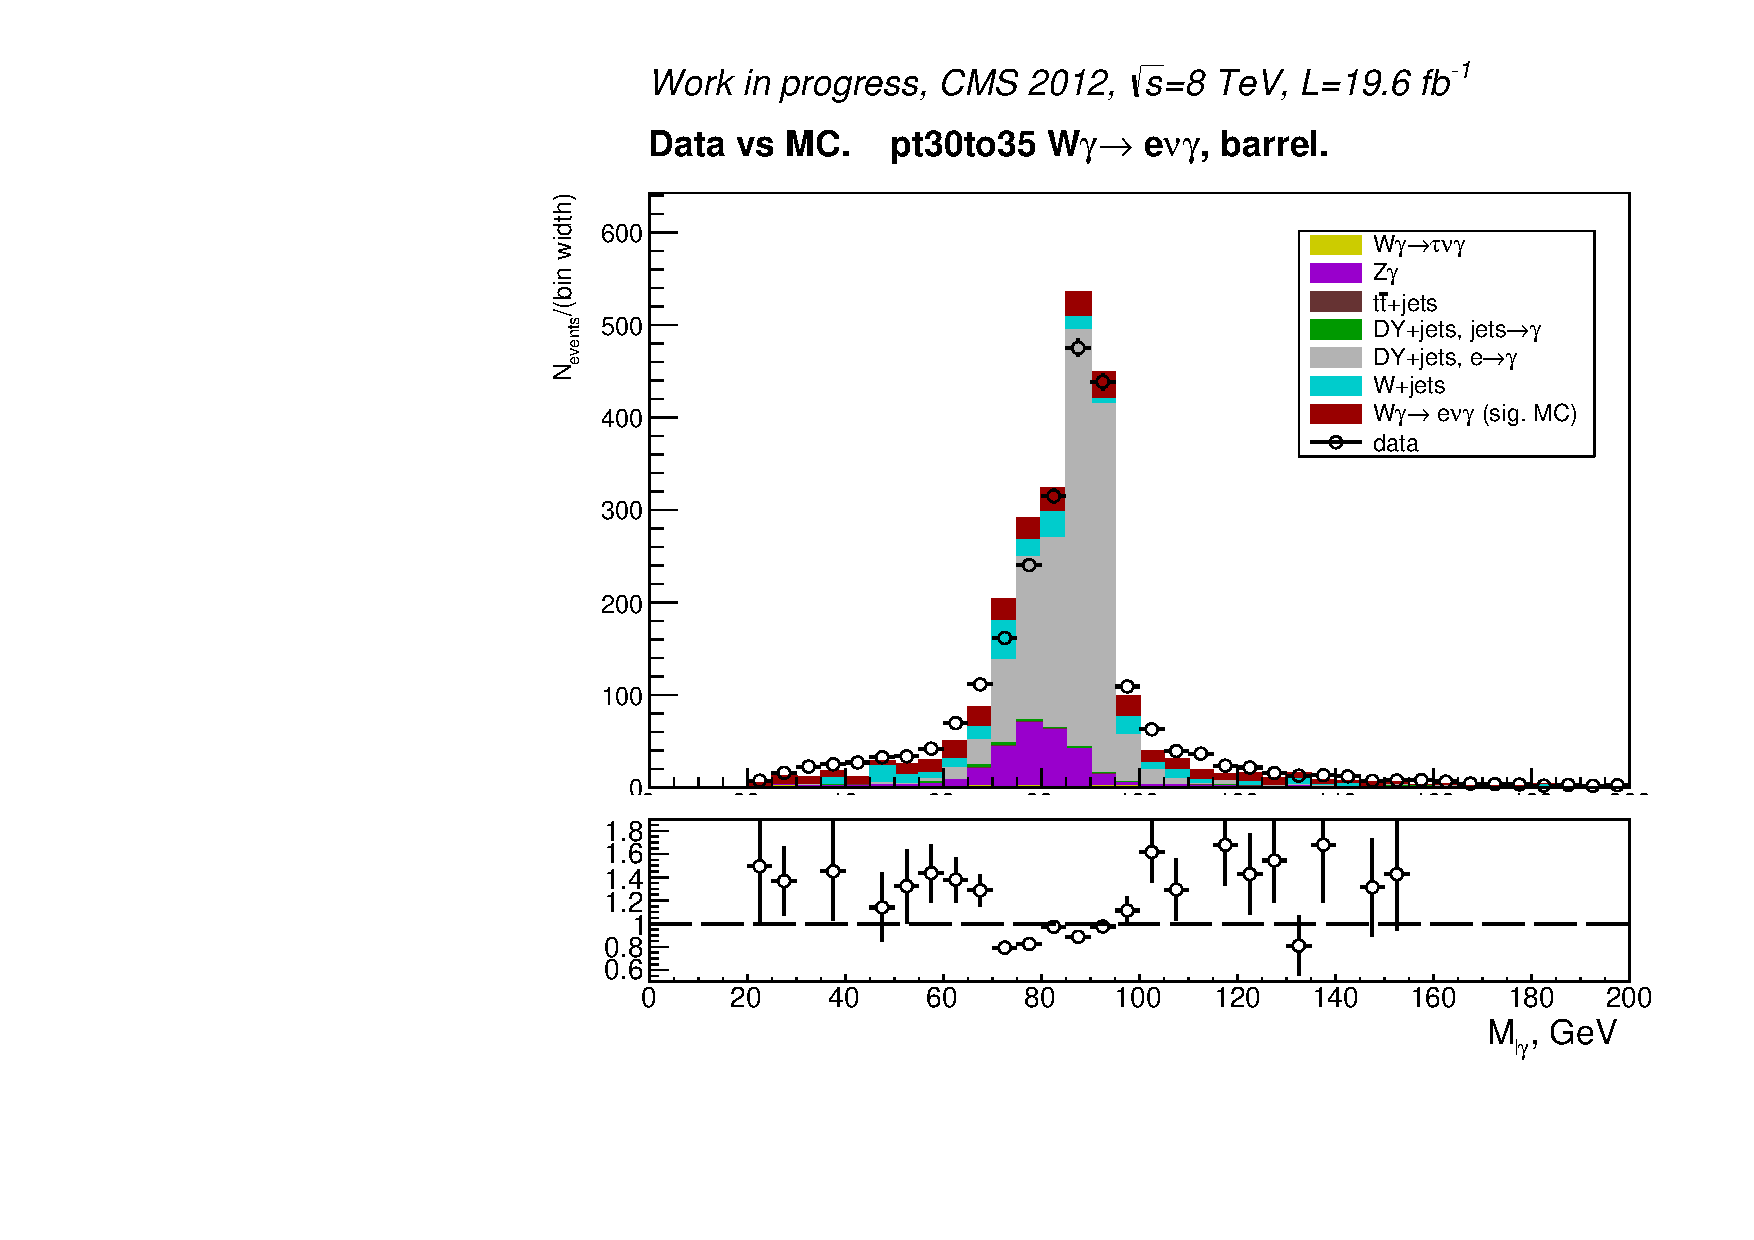
\includegraphics[width=0.40\textwidth]{../figs/figs_v11/ELECTRON_WGamma/PrepareYields/c_TotalDATAvsMC_Barrel__Mpholep1PRELIMINARY_FOR_E_TO_GAMMA_WITH_PSV_CUT_pt30to35__etogScale.pdf}   \\
    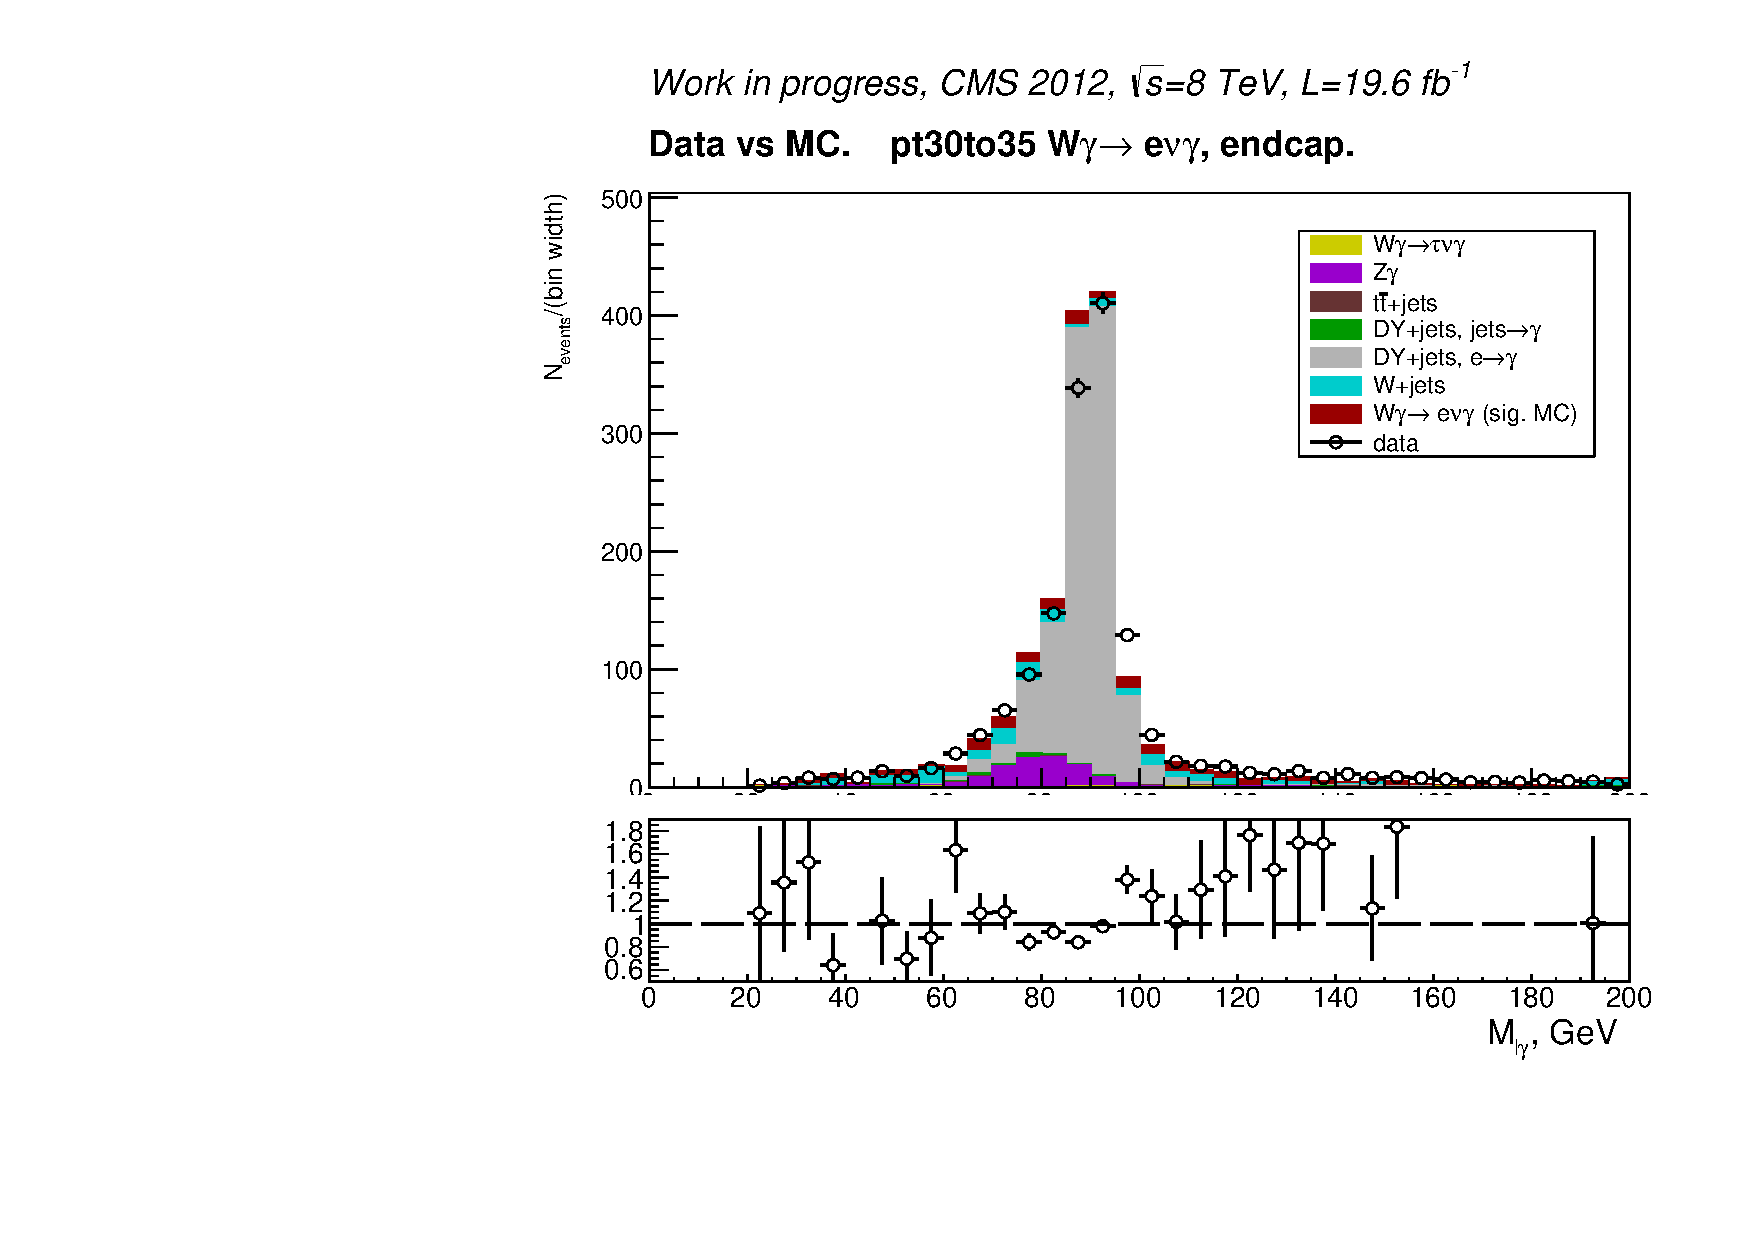
\includegraphics[width=0.40\textwidth]{../figs/figs_v11/ELECTRON_WGamma/PrepareYields/c_TotalDATAvsMC_Endcap__Mpholep1PRELIMINARY_FOR_E_TO_GAMMA_WITH_PSV_CUT_pt30to35_.pdf} 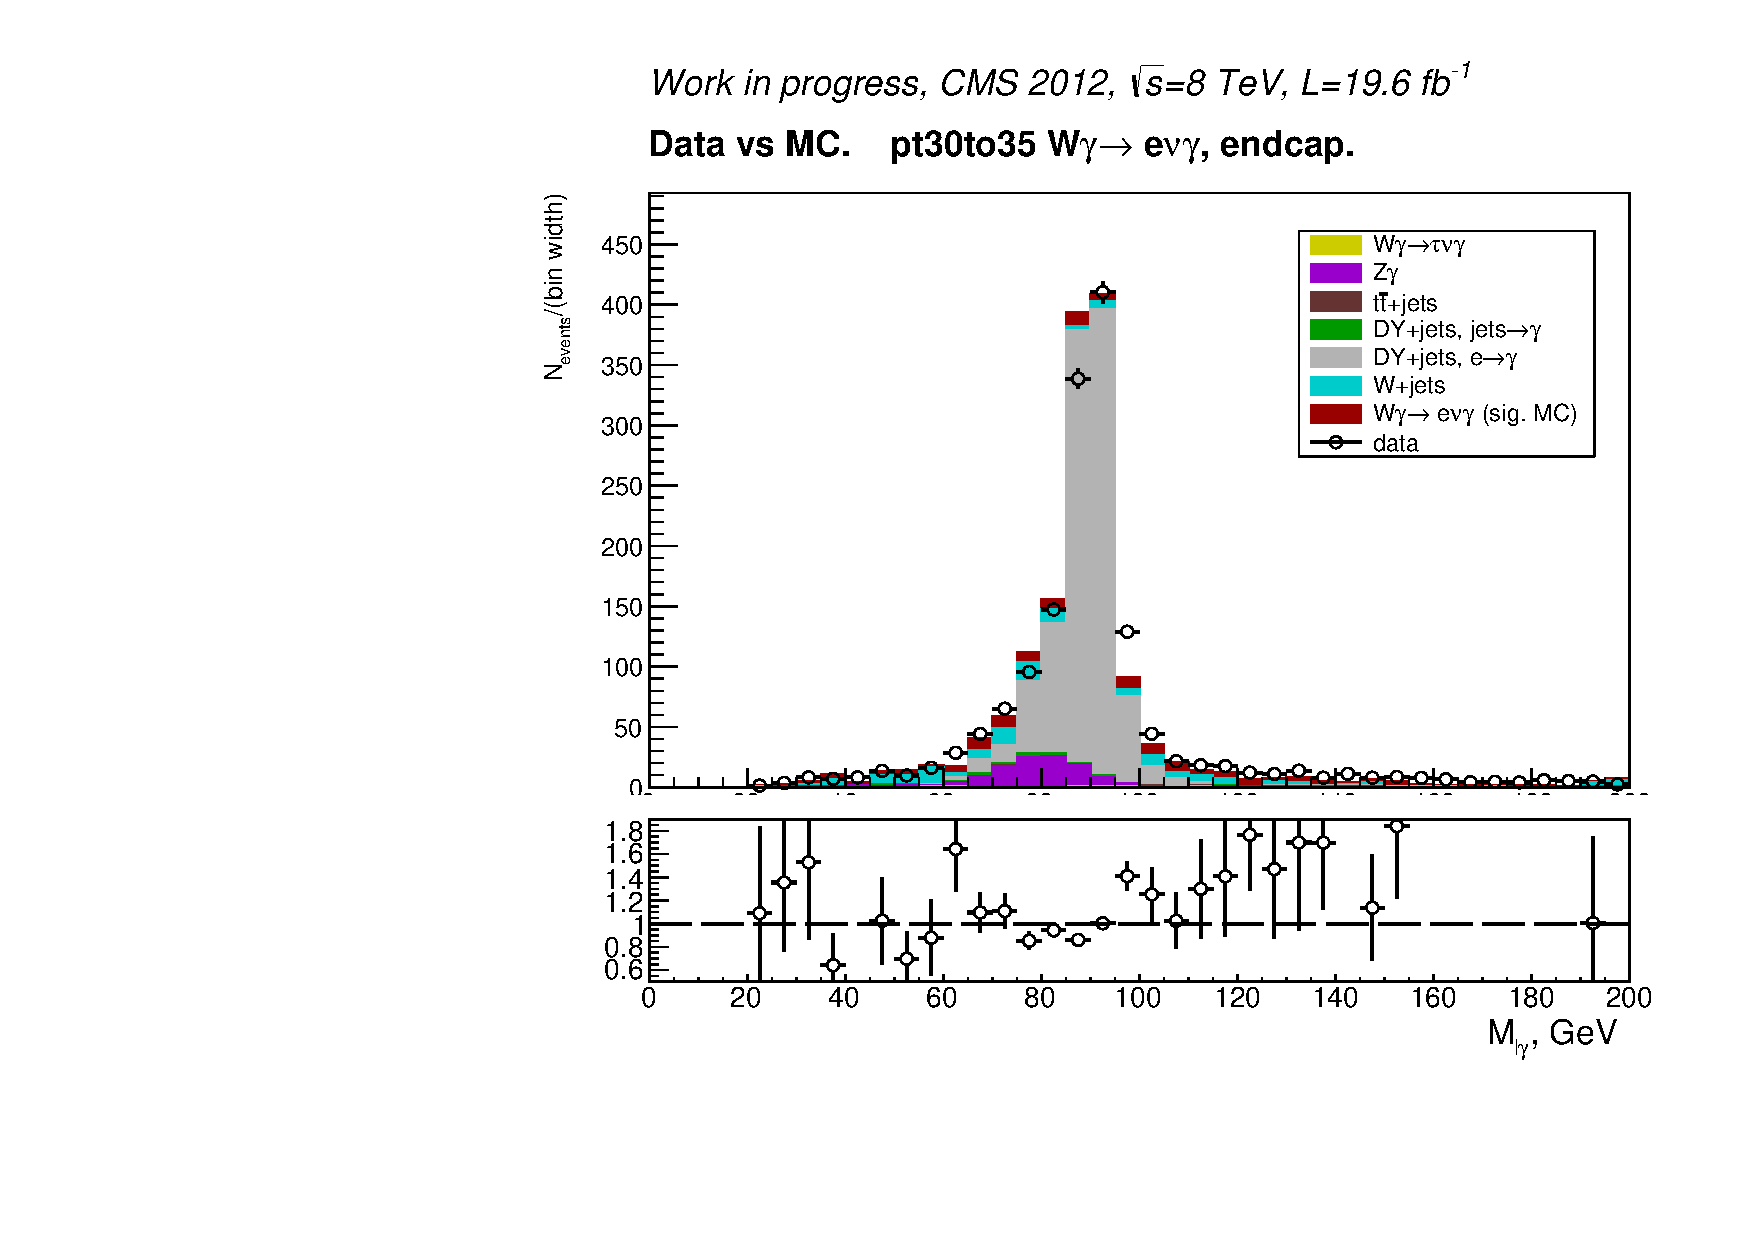
\includegraphics[width=0.40\textwidth]{../figs/figs_v11/ELECTRON_WGamma/PrepareYields/c_TotalDATAvsMC_Endcap__Mpholep1PRELIMINARY_FOR_E_TO_GAMMA_WITH_PSV_CUT_pt30to35__etogScale.pdf}\\
   \label{fig:Mpholep1DatavsMC_25to35}
  \caption{$M_{e,\gamma}$ distribution, data vs MC. Bins 25-30-35 GeV. Left: all MC samples are normalized to luminocity of data, PU weight adn SFs, right: DY$\rightarrow$jets(e$\rightarrow\gamma$) also normalized to e$\rightarrow\gamma$ data-driven estimates.}
  \end{center}
\end{figure}

\begin{figure}[htb]
  \begin{center}
    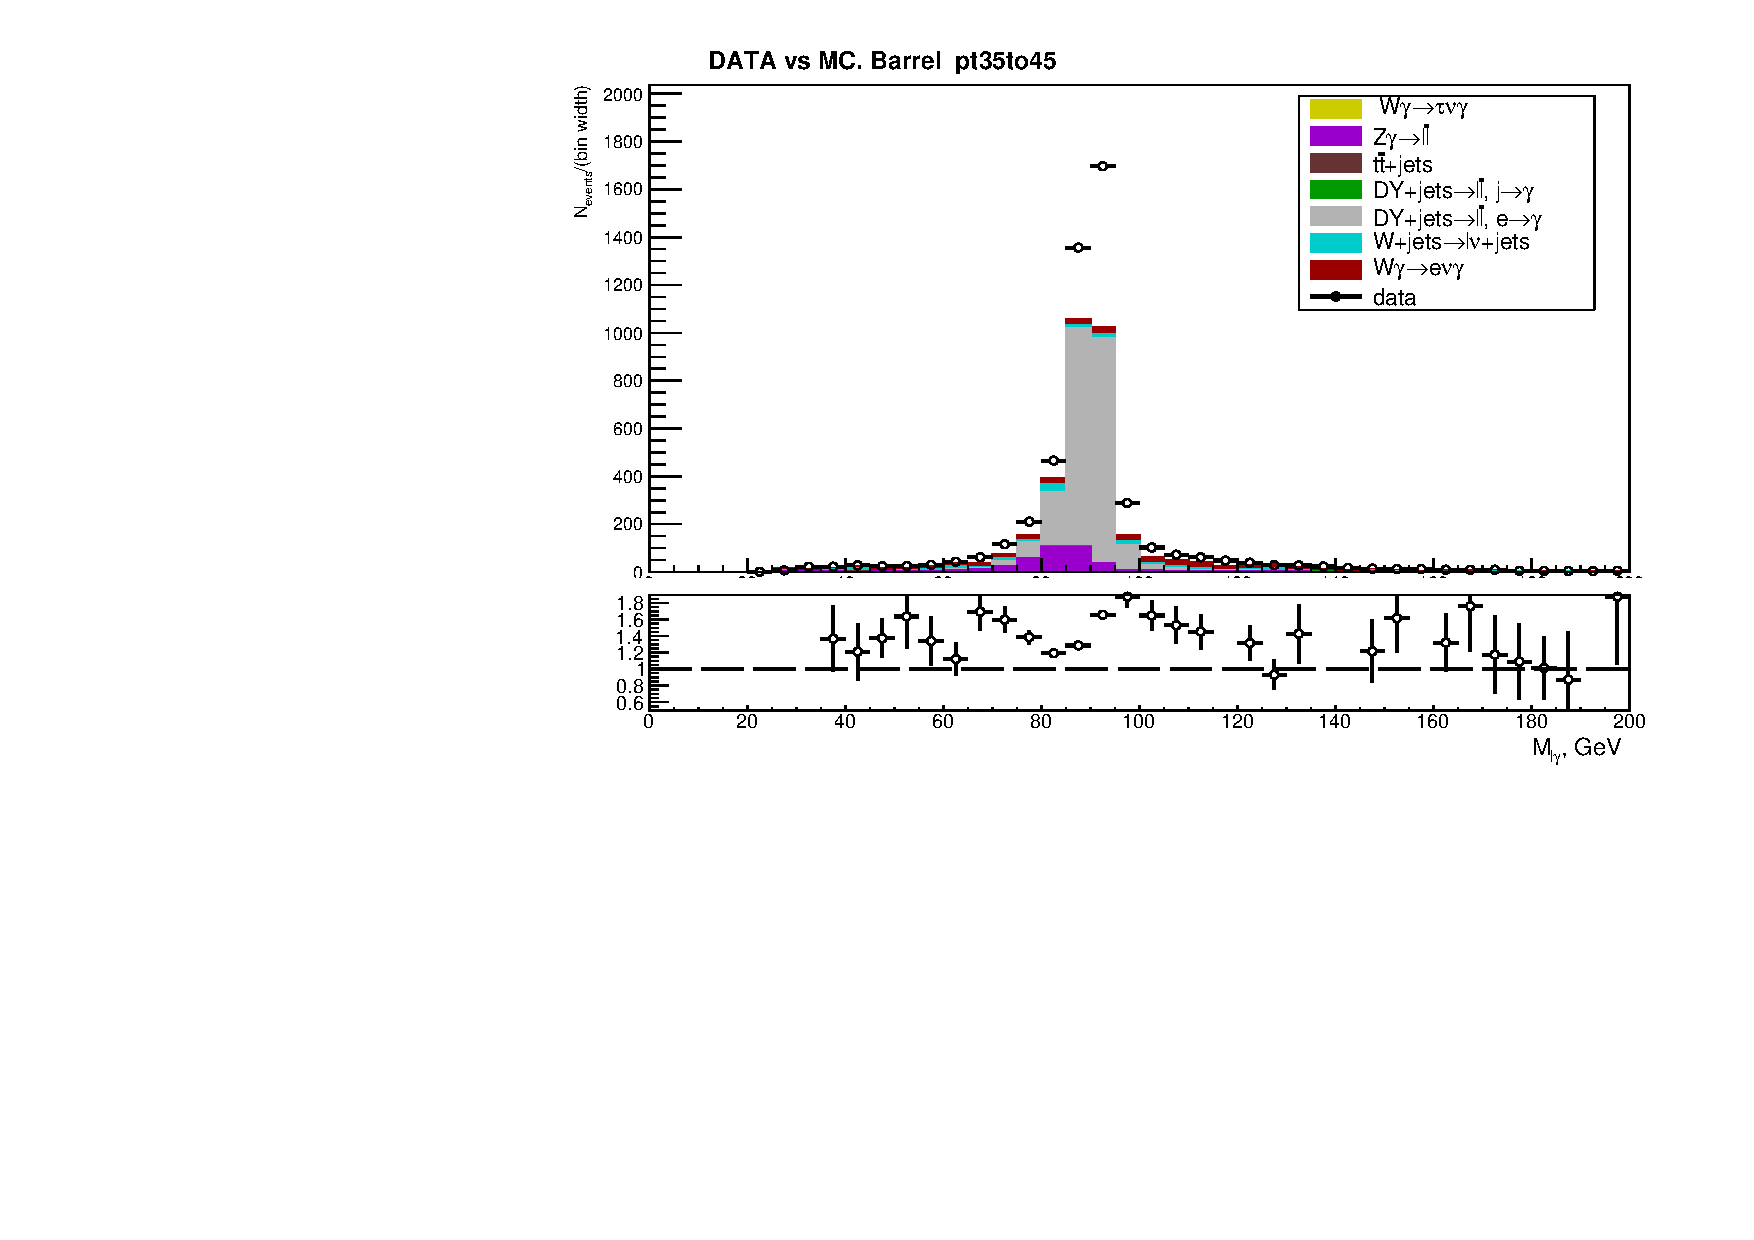
\includegraphics[width=0.40\textwidth]{../figs/figs_v11/ELECTRON_WGamma/PrepareYields/c_TotalDATAvsMC_Barrel__Mpholep1PRELIMINARY_FOR_E_TO_GAMMA_WITH_PSV_CUT_pt35to45_.pdf}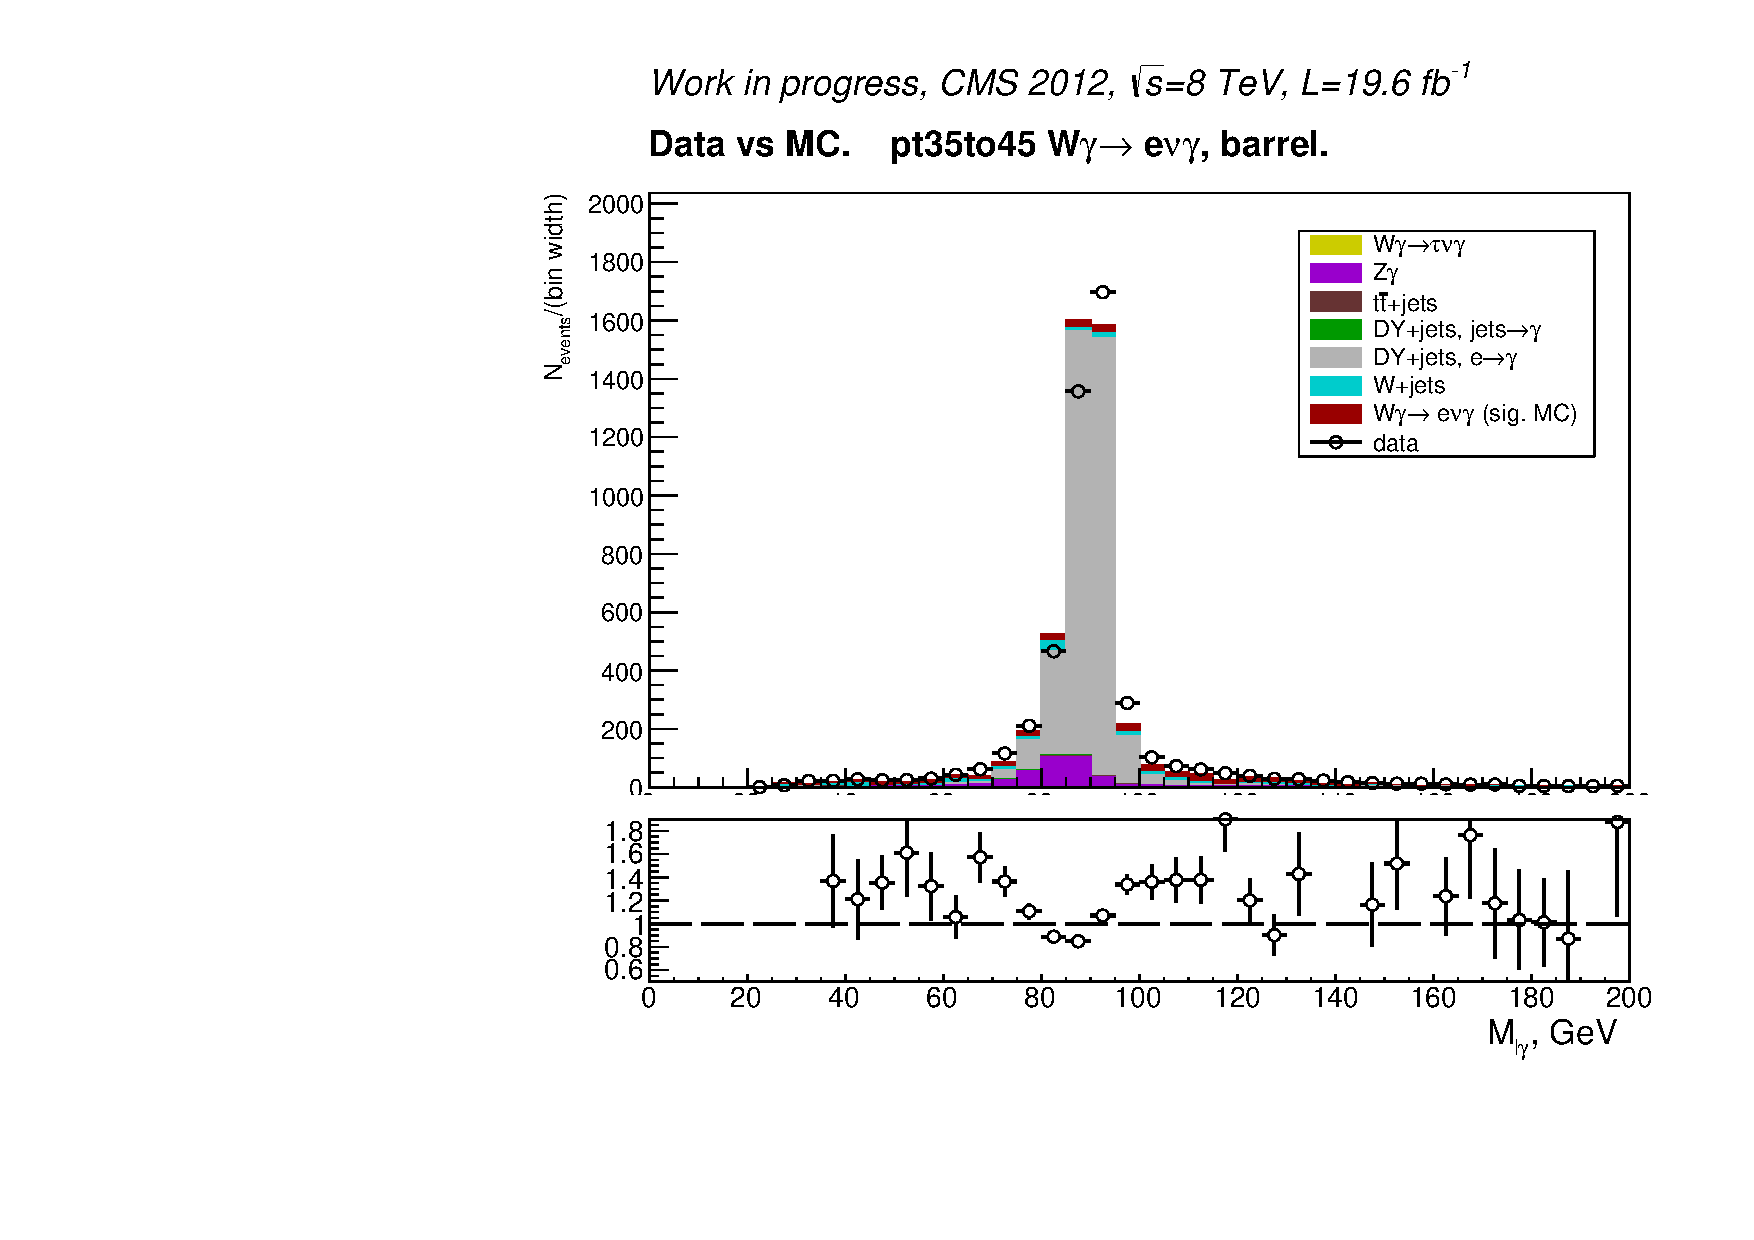
\includegraphics[width=0.40\textwidth]{../figs/figs_v11/ELECTRON_WGamma/PrepareYields/c_TotalDATAvsMC_Barrel__Mpholep1PRELIMINARY_FOR_E_TO_GAMMA_WITH_PSV_CUT_pt35to45__etogScale.pdf}\\
    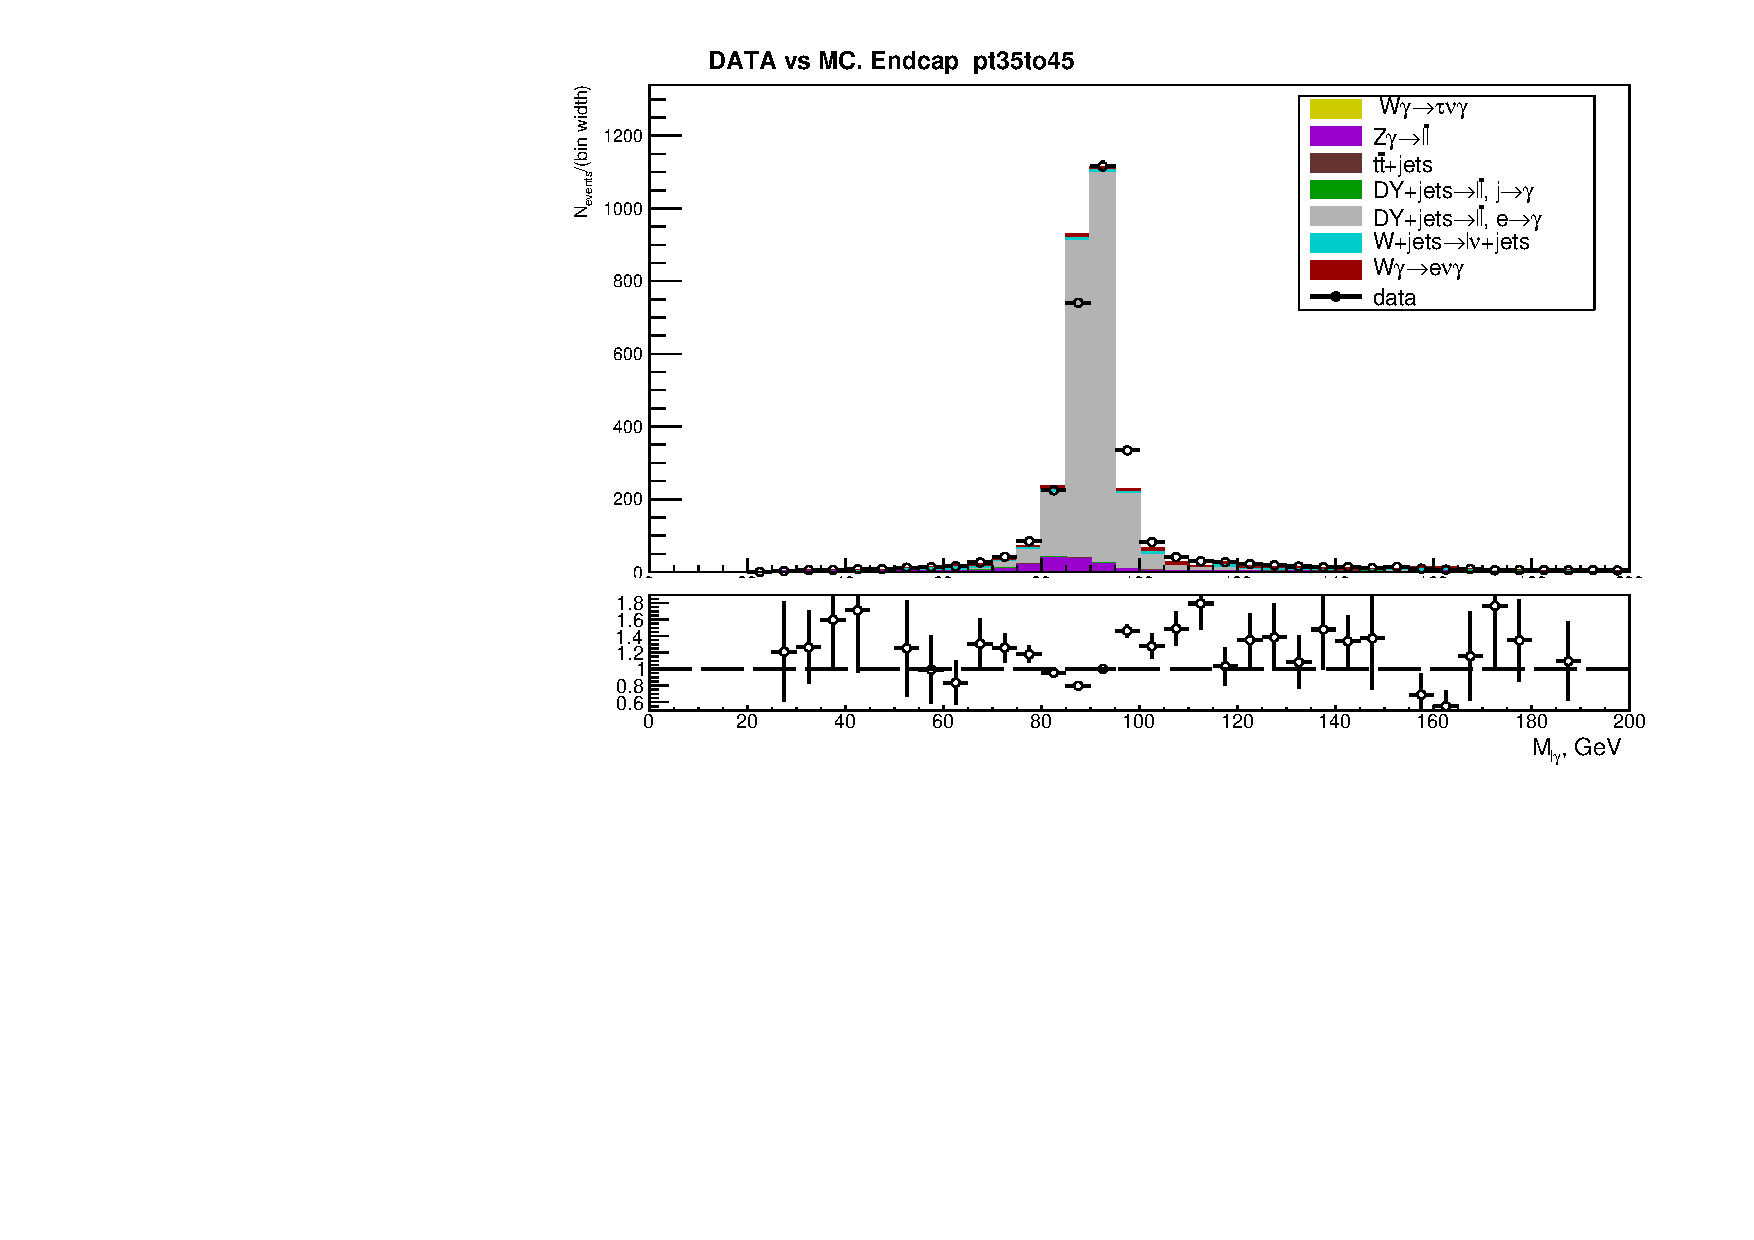
\includegraphics[width=0.40\textwidth]{../figs/figs_v11/ELECTRON_WGamma/PrepareYields/c_TotalDATAvsMC_Endcap__Mpholep1PRELIMINARY_FOR_E_TO_GAMMA_WITH_PSV_CUT_pt35to45_.pdf}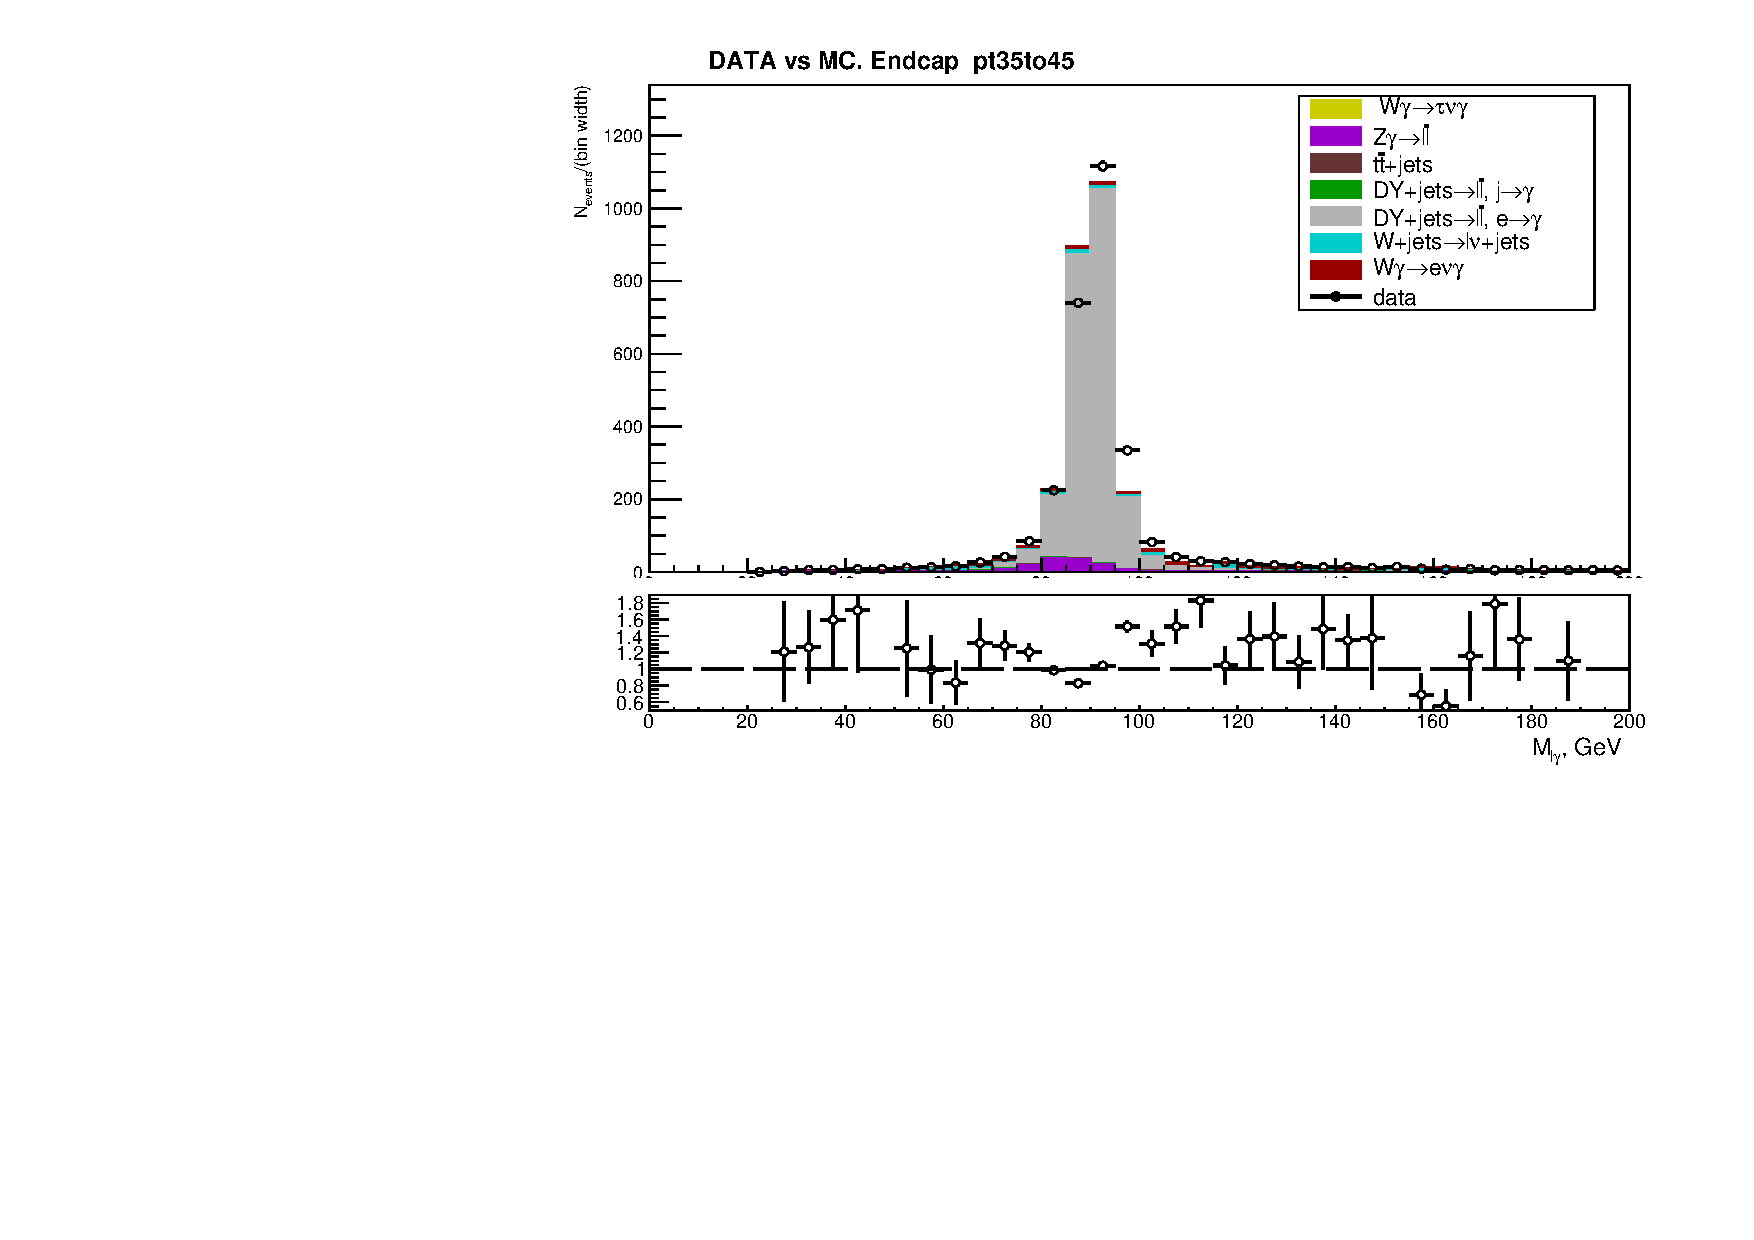
\includegraphics[width=0.40\textwidth]{../figs/figs_v11/ELECTRON_WGamma/PrepareYields/c_TotalDATAvsMC_Endcap__Mpholep1PRELIMINARY_FOR_E_TO_GAMMA_WITH_PSV_CUT_pt35to45__etogScale.pdf}\\
    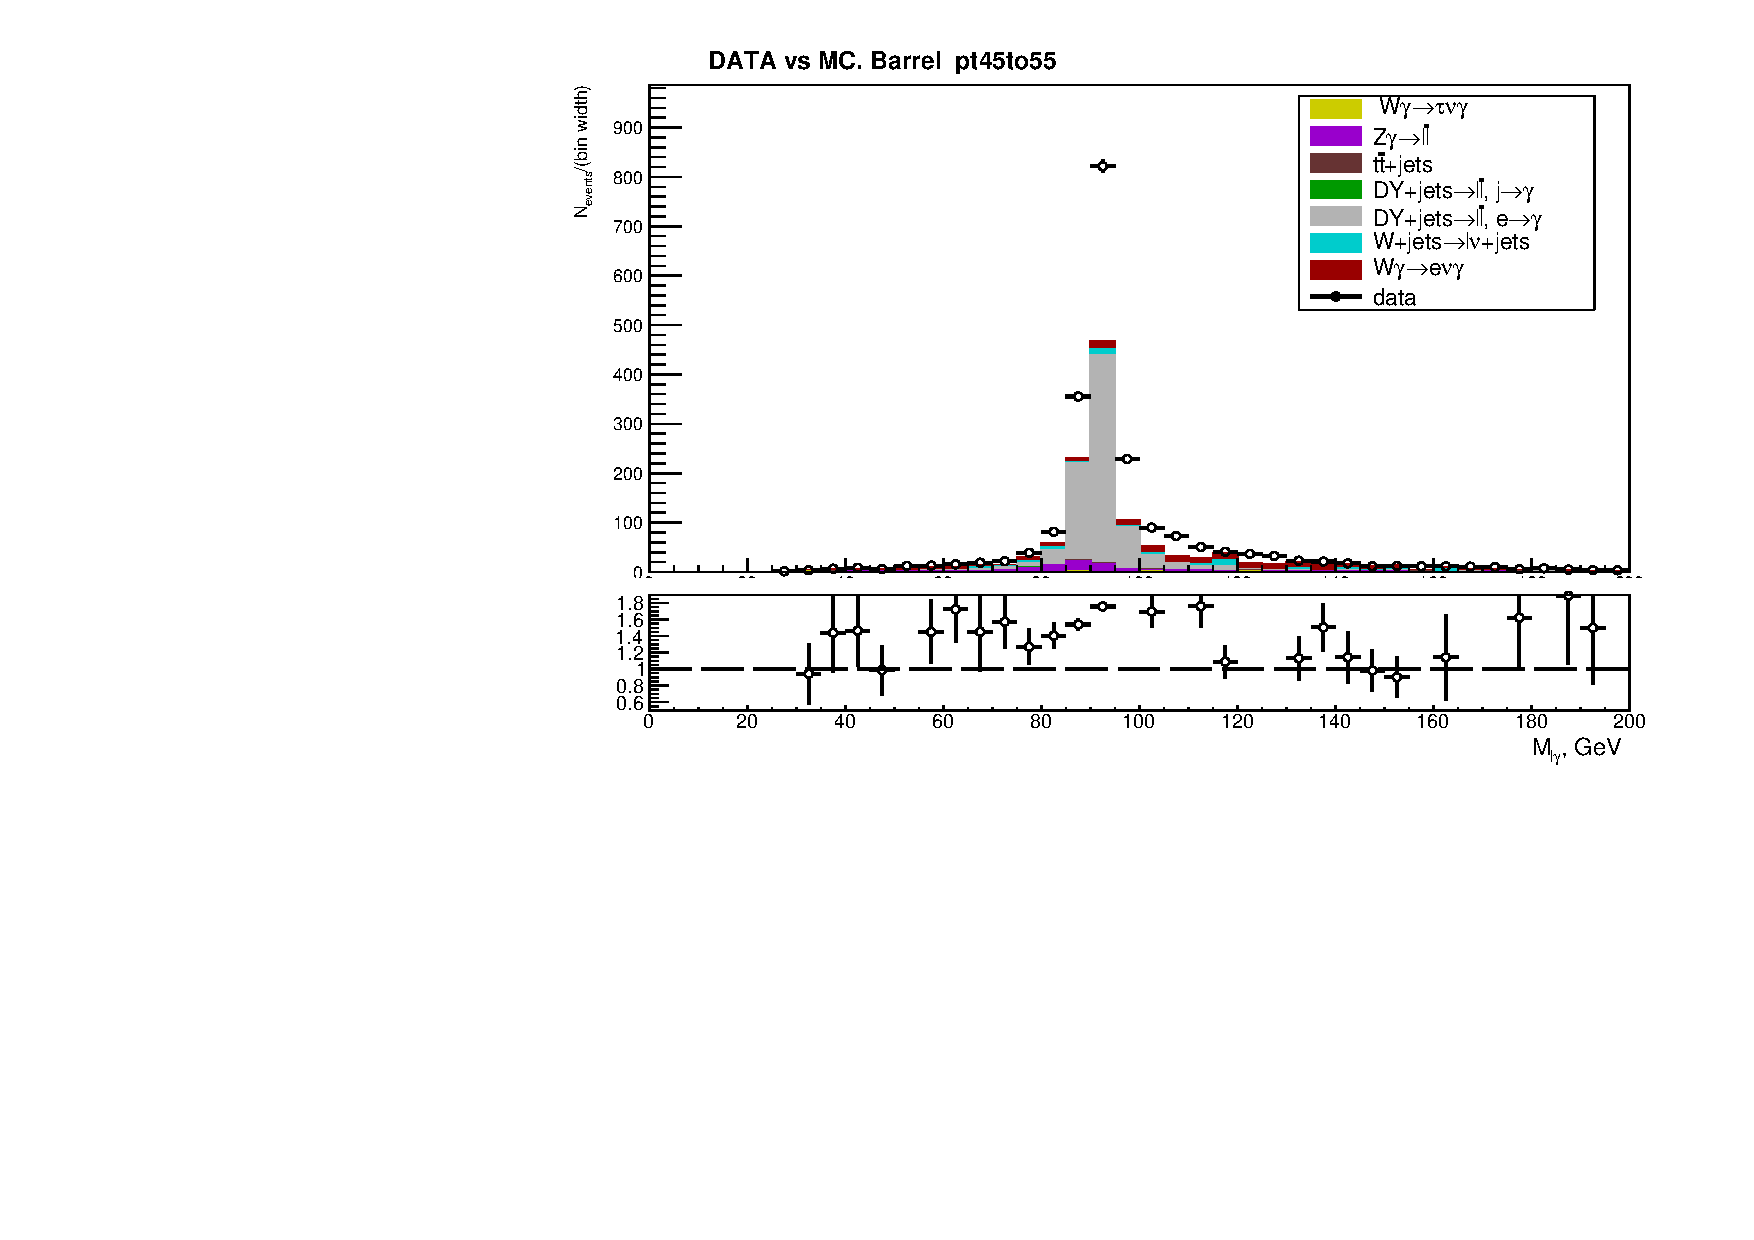
\includegraphics[width=0.40\textwidth]{../figs/figs_v11/ELECTRON_WGamma/PrepareYields/c_TotalDATAvsMC_Barrel__Mpholep1PRELIMINARY_FOR_E_TO_GAMMA_WITH_PSV_CUT_pt45to55_.pdf}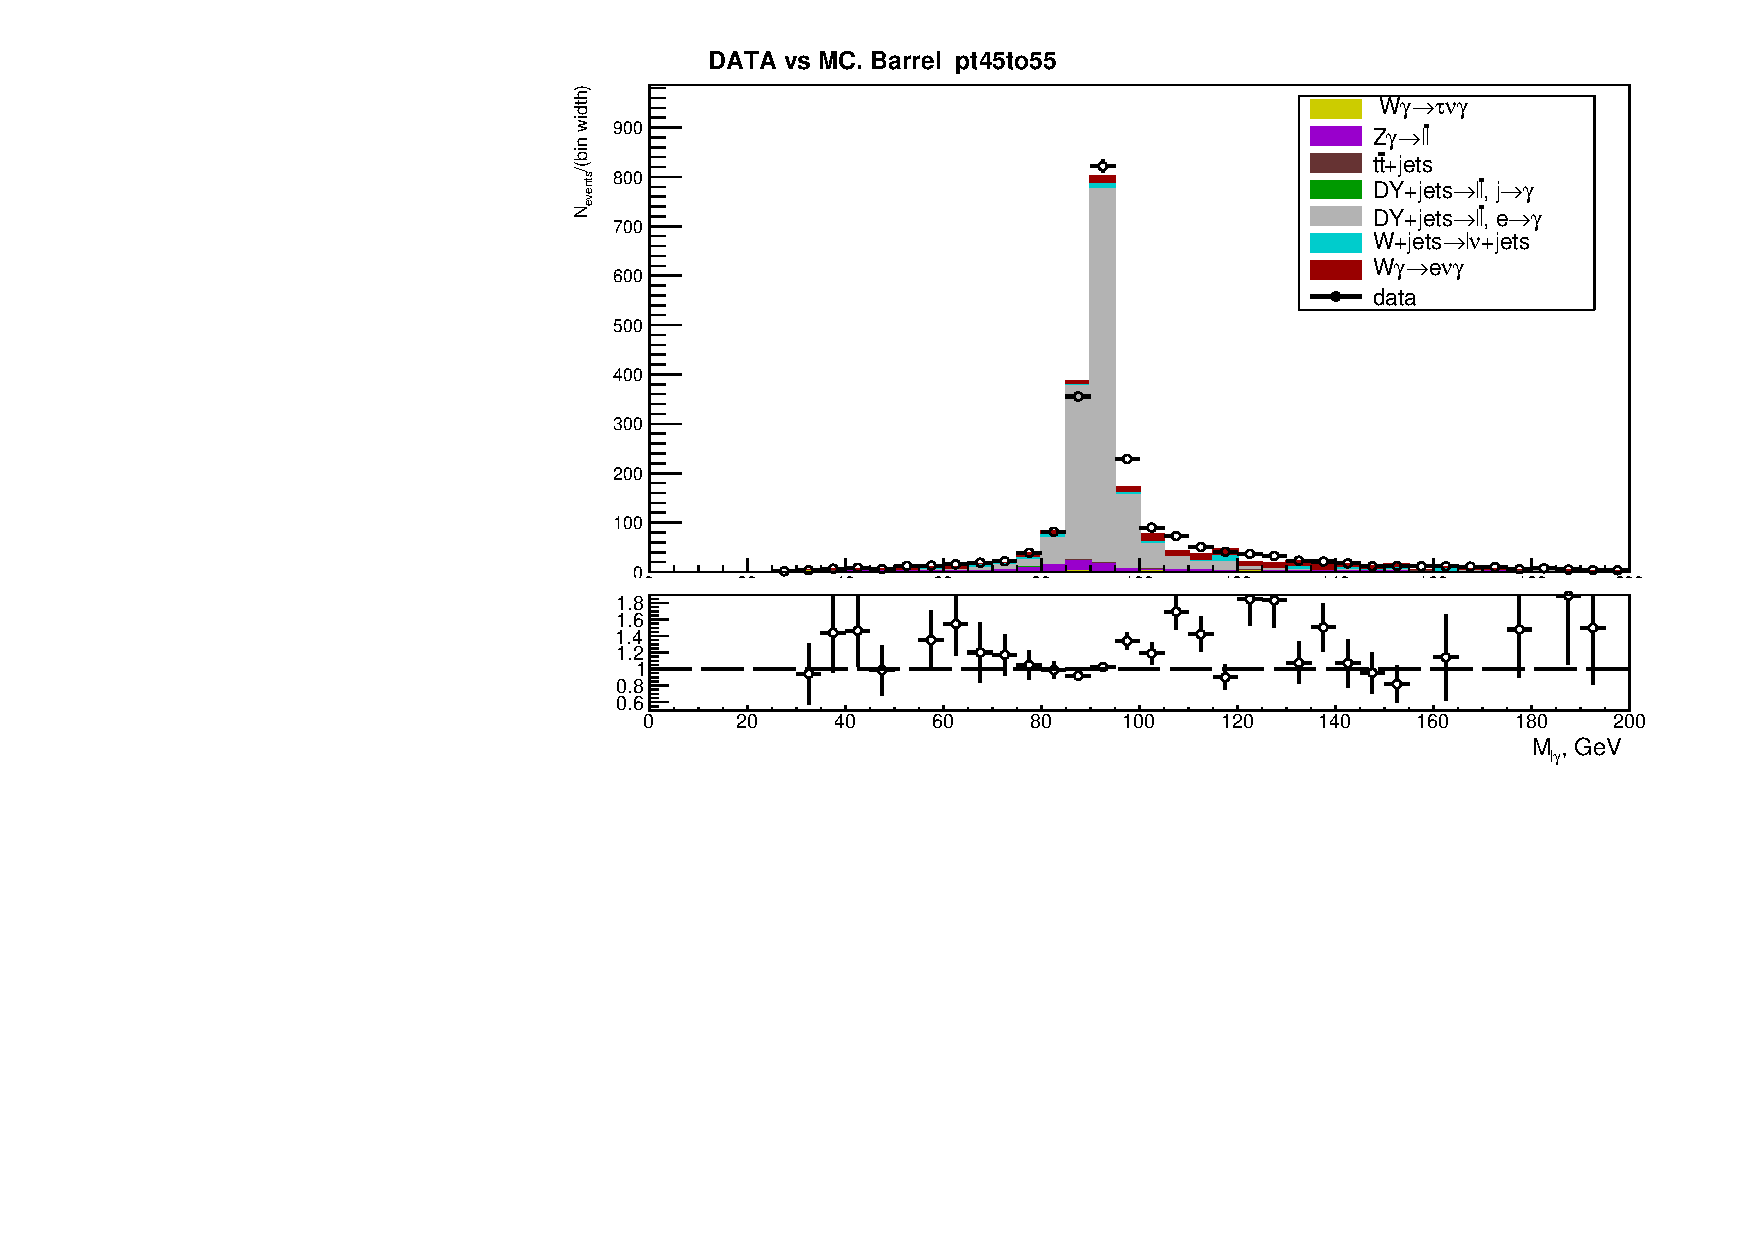
\includegraphics[width=0.40\textwidth]{../figs/figs_v11/ELECTRON_WGamma/PrepareYields/c_TotalDATAvsMC_Barrel__Mpholep1PRELIMINARY_FOR_E_TO_GAMMA_WITH_PSV_CUT_pt45to55__etogScale.pdf}\\
    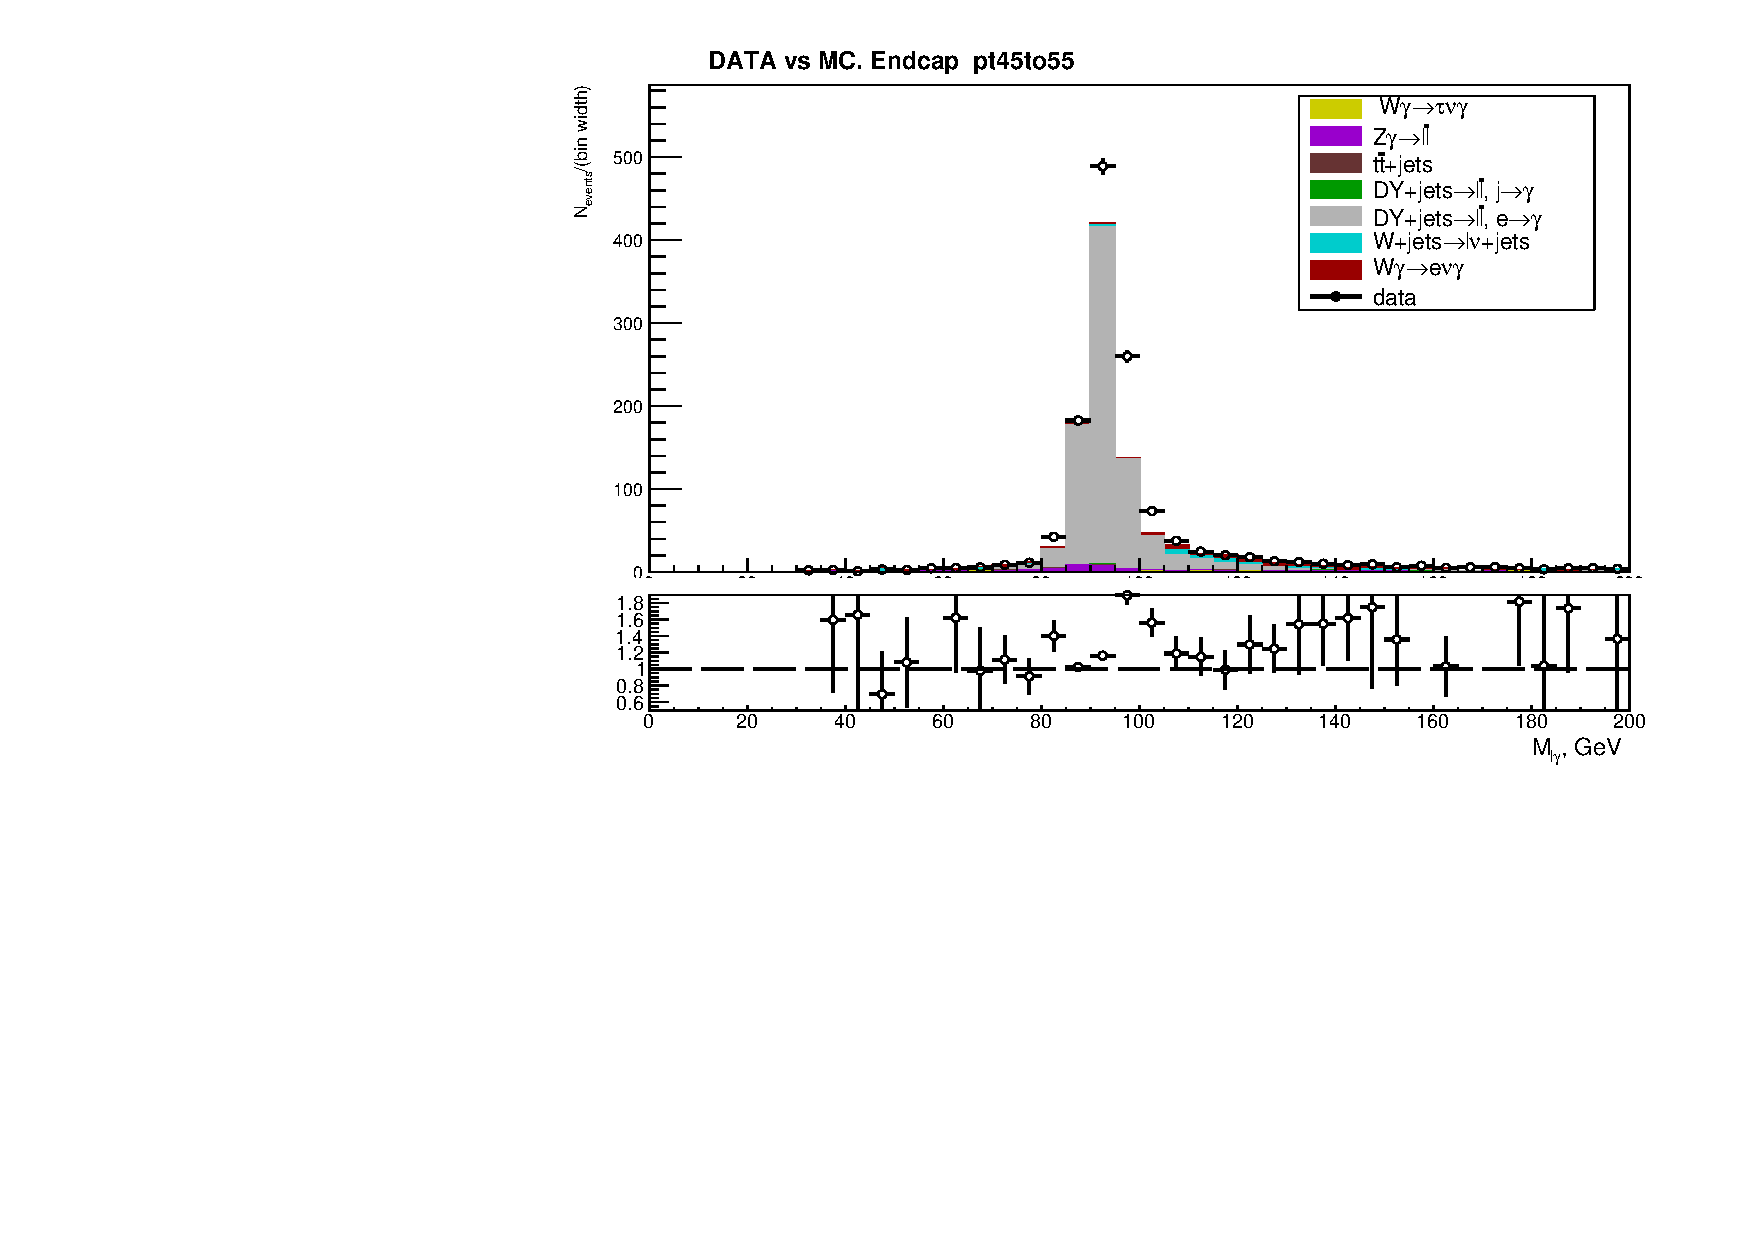
\includegraphics[width=0.40\textwidth]{../figs/figs_v11/ELECTRON_WGamma/PrepareYields/c_TotalDATAvsMC_Endcap__Mpholep1PRELIMINARY_FOR_E_TO_GAMMA_WITH_PSV_CUT_pt45to55_.pdf}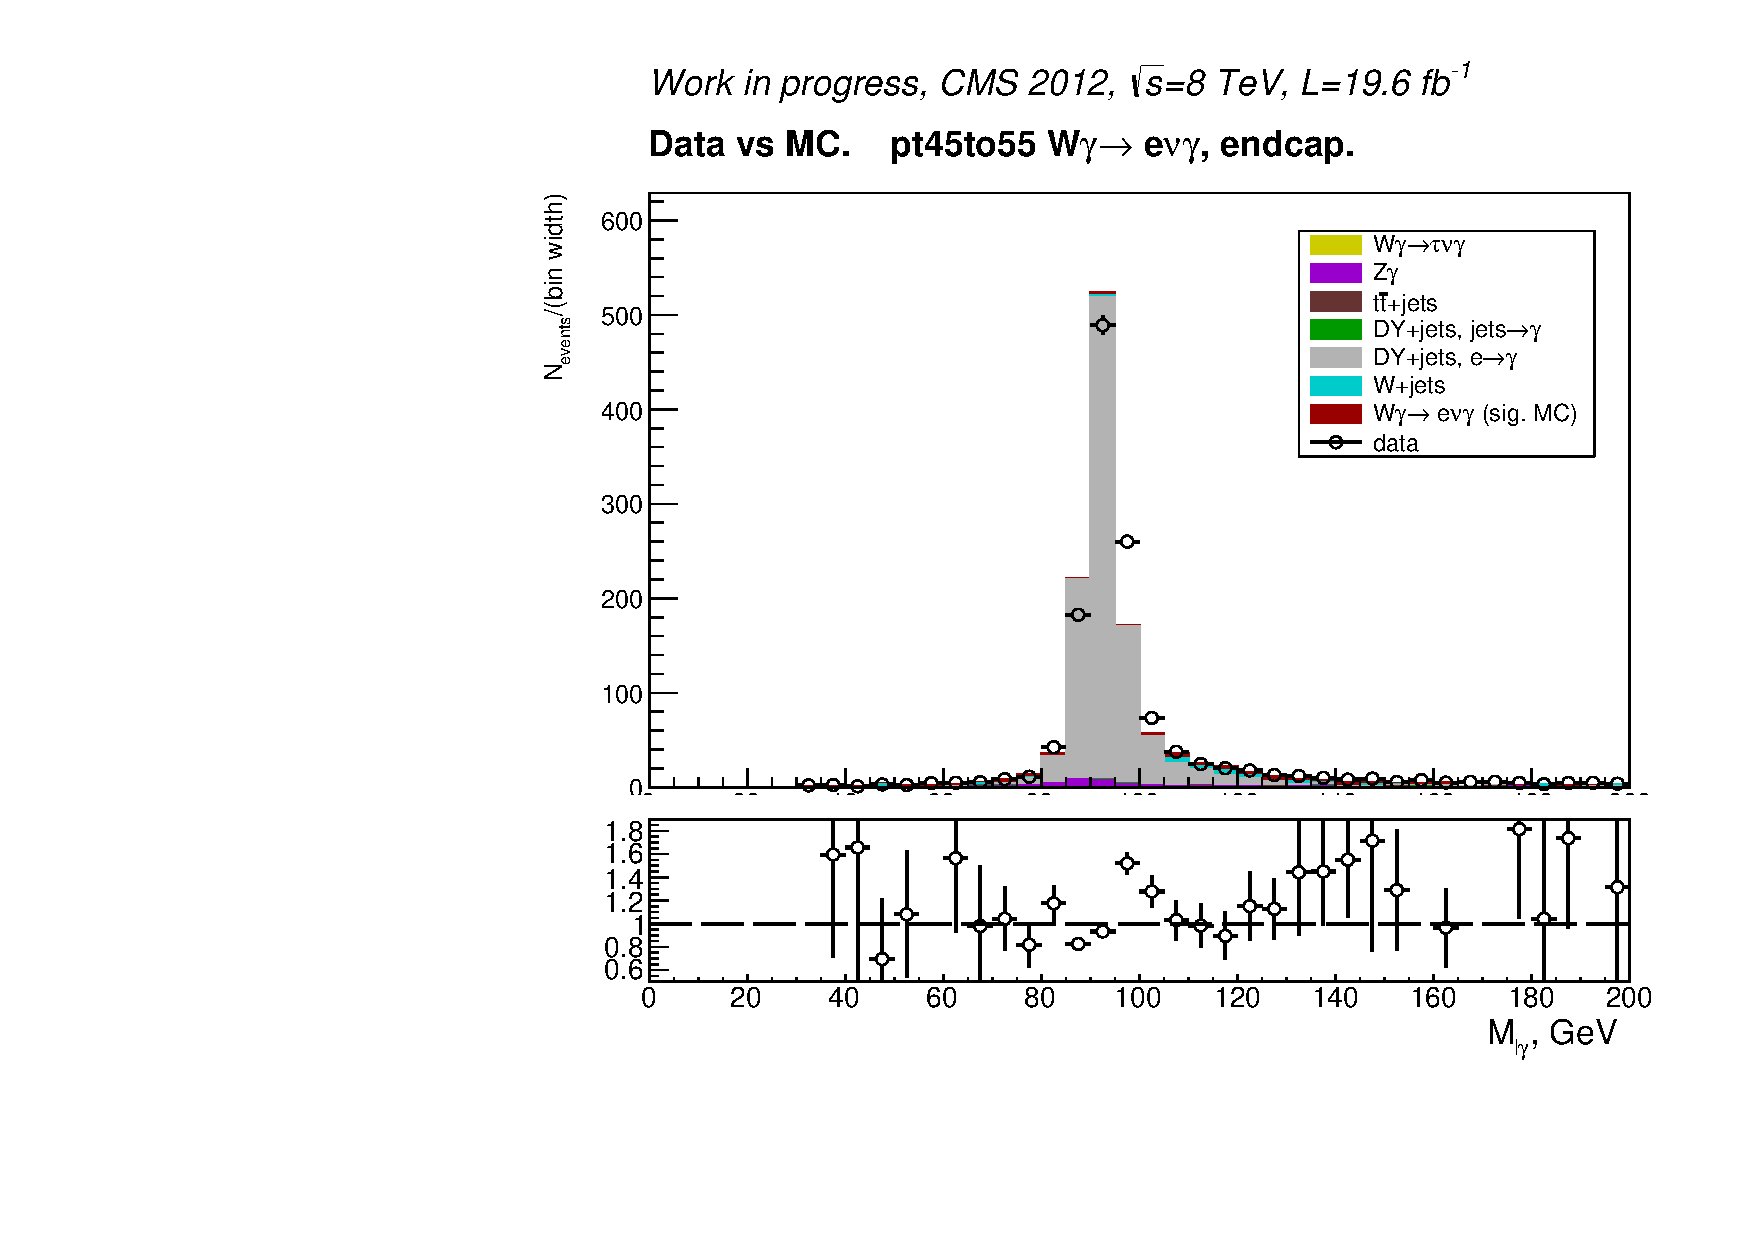
\includegraphics[width=0.40\textwidth]{../figs/figs_v11/ELECTRON_WGamma/PrepareYields/c_TotalDATAvsMC_Endcap__Mpholep1PRELIMINARY_FOR_E_TO_GAMMA_WITH_PSV_CUT_pt45to55__etogScale.pdf}\\
   \label{fig:Mpholep1DatavsMC_35to75}
  \caption{$M_{e,\gamma}$ distribution, data vs MC. Bins 35-45-55 GeV. Left: all MC samples are normalized to luminocity of data, PU weight adn SFs, right: DY$\rightarrow$jets(e$\rightarrow\gamma$) also normalized to e$\rightarrow\gamma$ data-driven estimates.}
  \end{center}
\end{figure}

\begin{figure}[htb]
  \begin{center}
    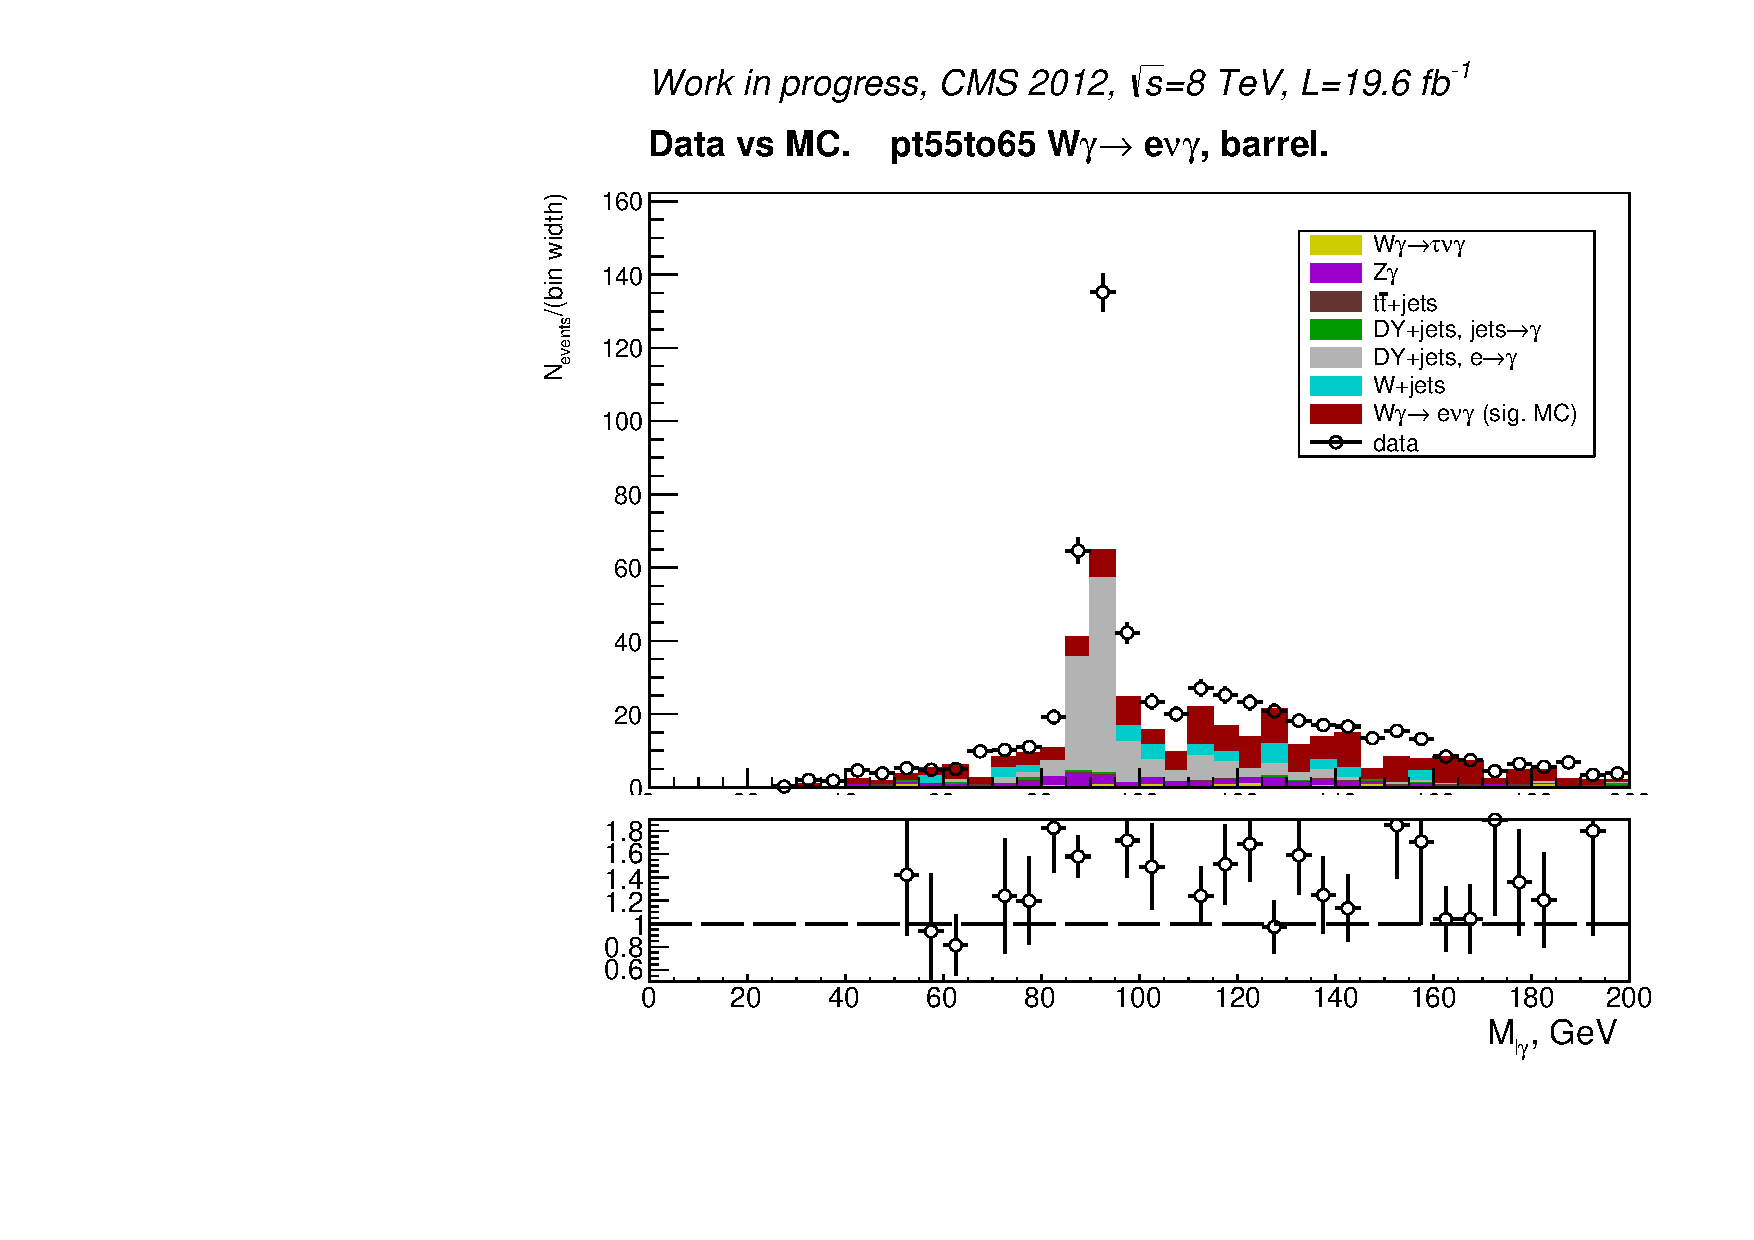
\includegraphics[width=0.40\textwidth]{../figs/figs_v11/ELECTRON_WGamma/PrepareYields/c_TotalDATAvsMC_Barrel__Mpholep1PRELIMINARY_FOR_E_TO_GAMMA_WITH_PSV_CUT_pt55to65_.pdf}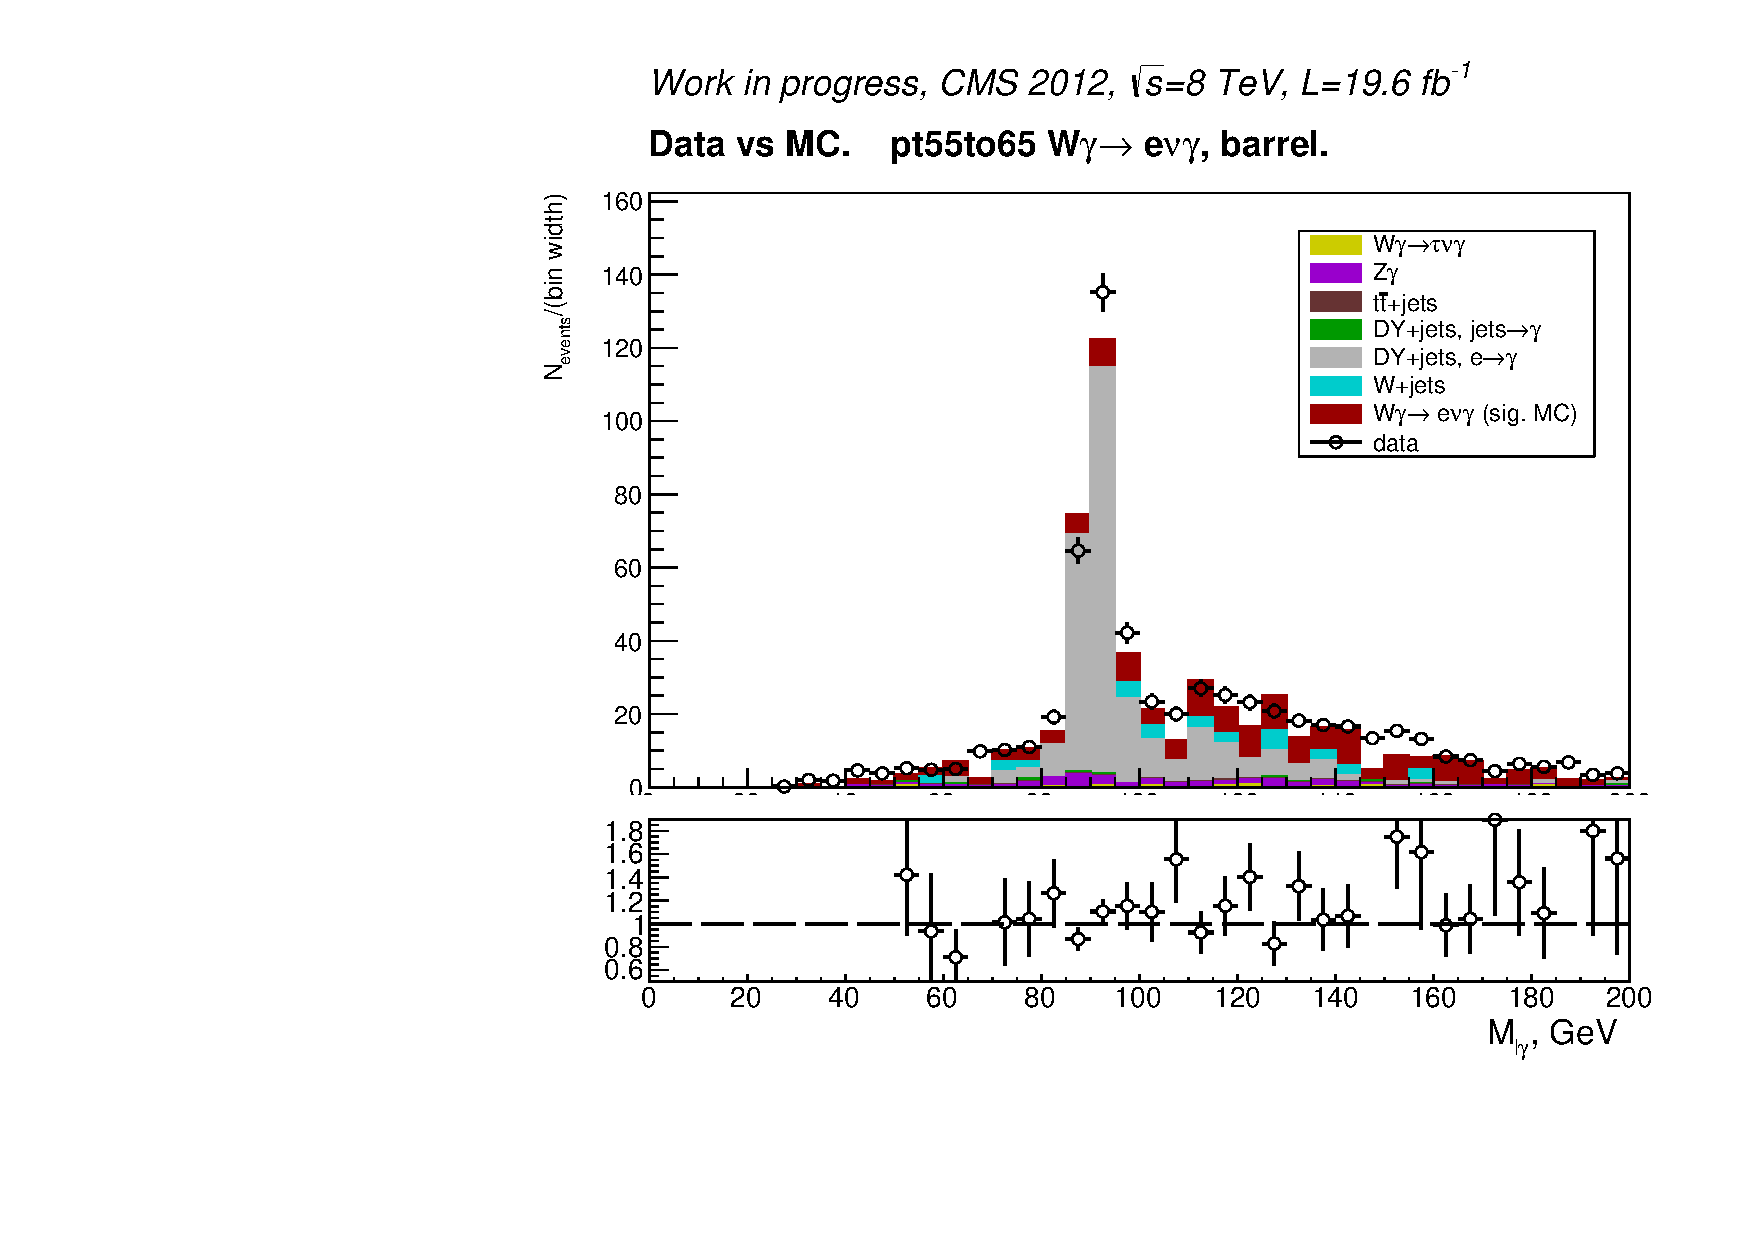
\includegraphics[width=0.40\textwidth]{../figs/figs_v11/ELECTRON_WGamma/PrepareYields/c_TotalDATAvsMC_Barrel__Mpholep1PRELIMINARY_FOR_E_TO_GAMMA_WITH_PSV_CUT_pt55to65__etogScale.pdf}\\    
    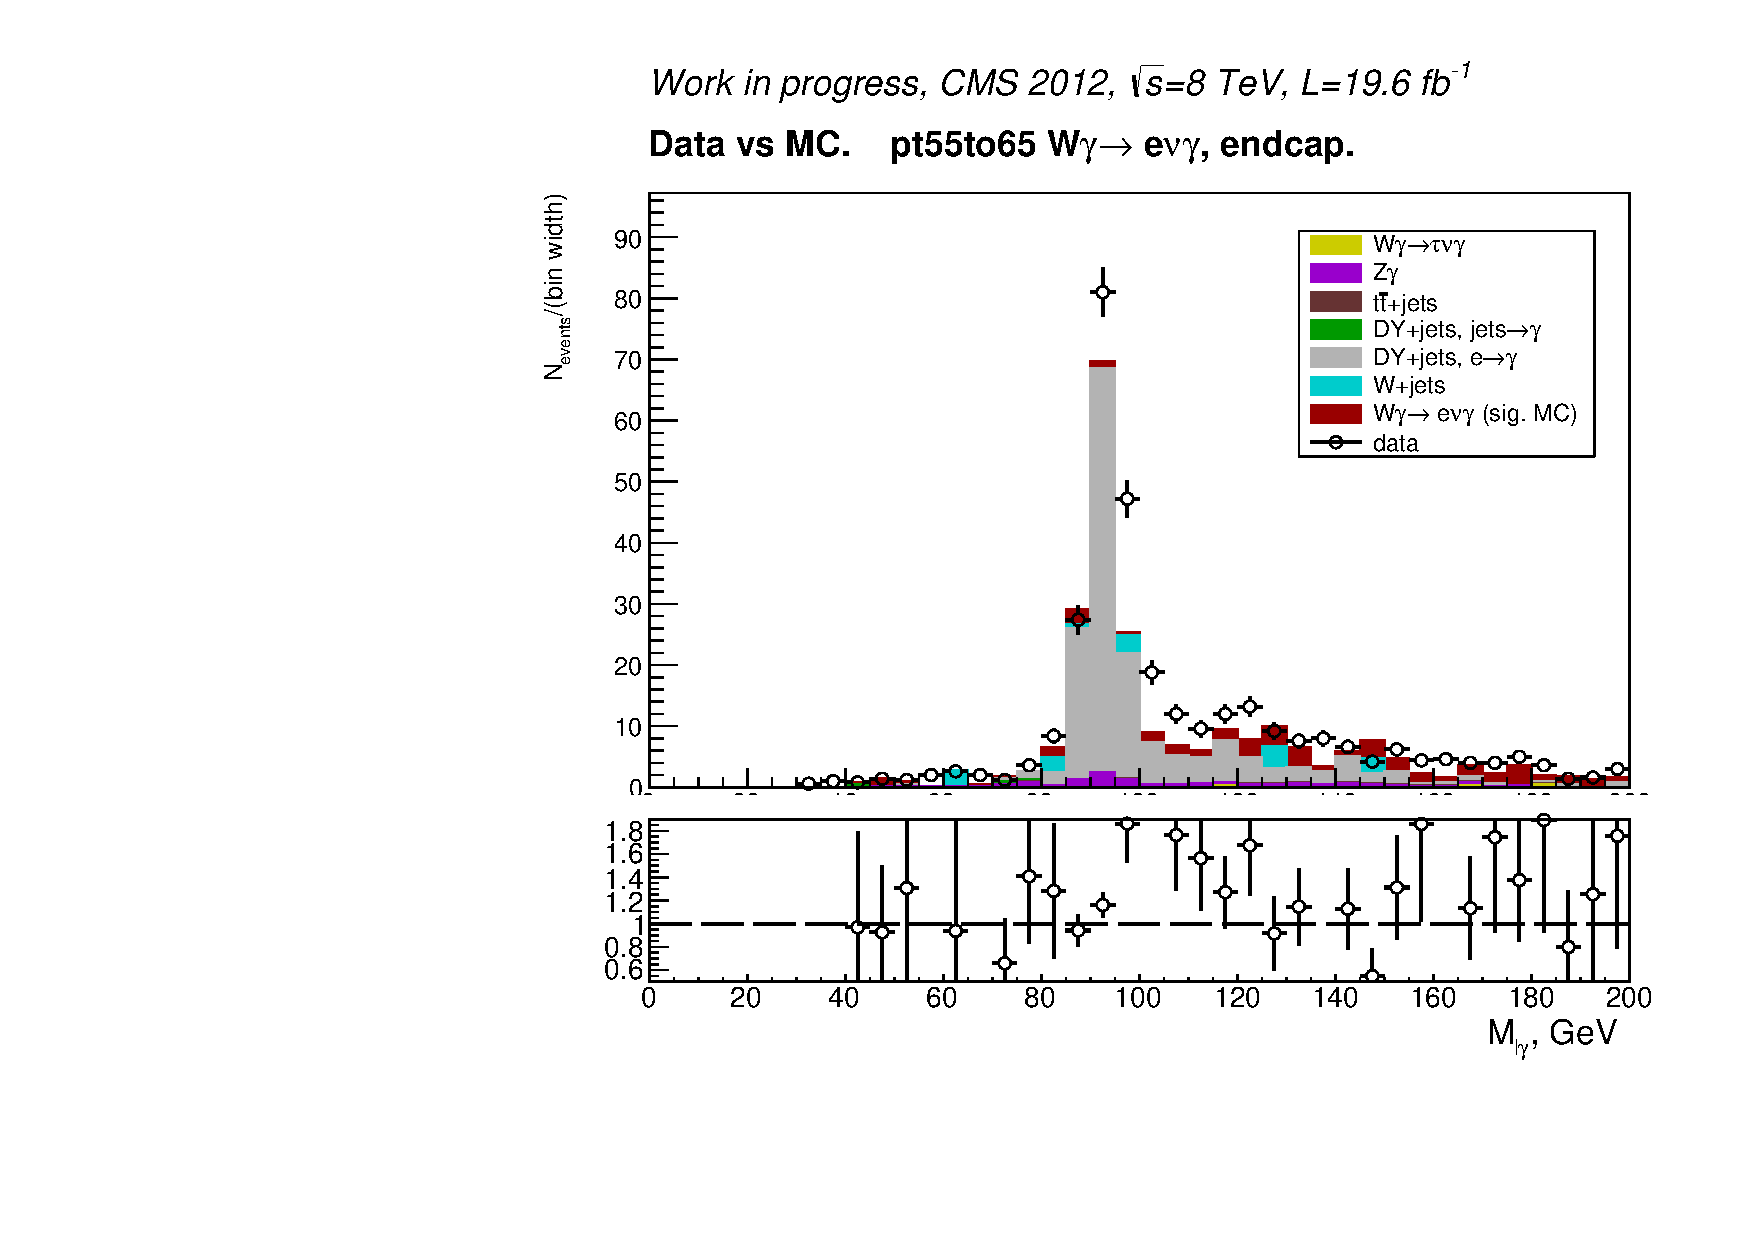
\includegraphics[width=0.40\textwidth]{../figs/figs_v11/ELECTRON_WGamma/PrepareYields/c_TotalDATAvsMC_Endcap__Mpholep1PRELIMINARY_FOR_E_TO_GAMMA_WITH_PSV_CUT_pt55to65_.pdf}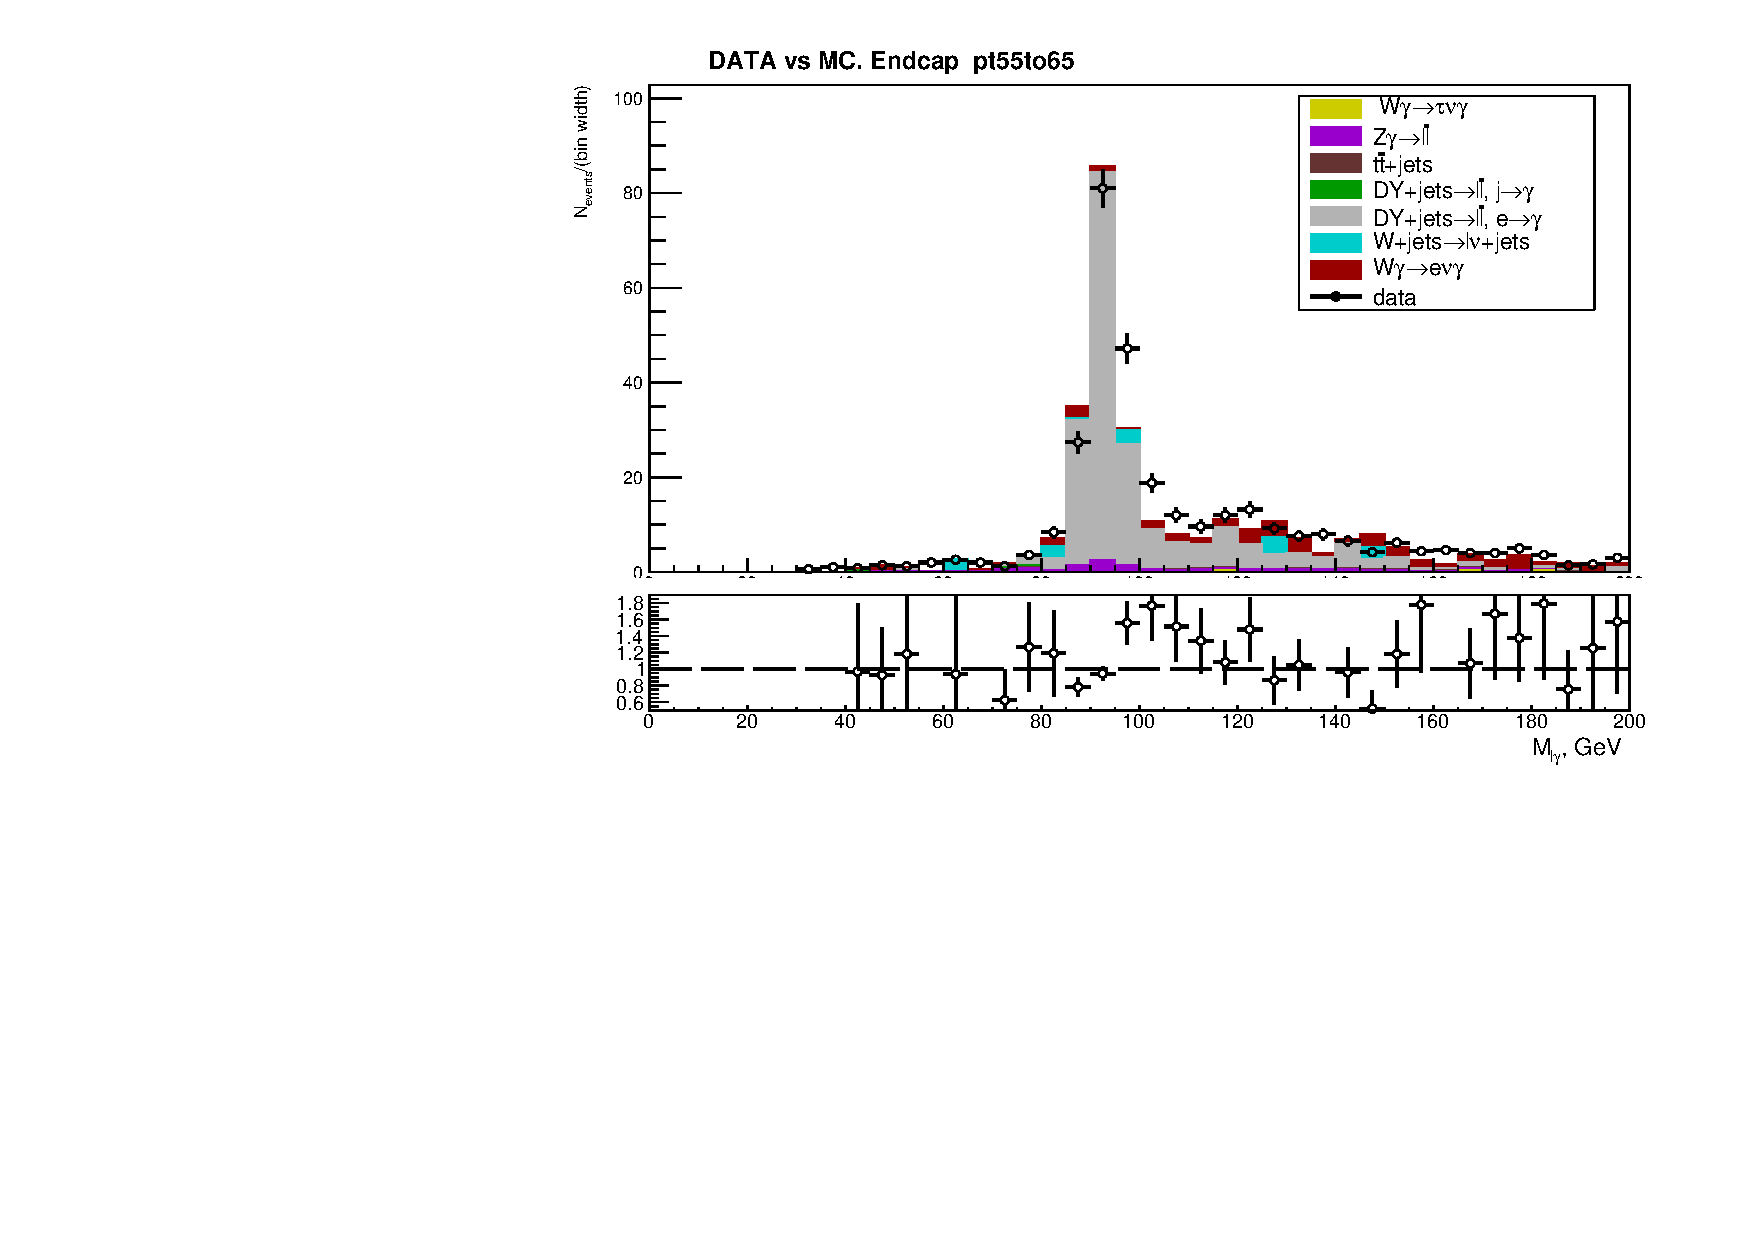
\includegraphics[width=0.40\textwidth]{../figs/figs_v11/ELECTRON_WGamma/PrepareYields/c_TotalDATAvsMC_Endcap__Mpholep1PRELIMINARY_FOR_E_TO_GAMMA_WITH_PSV_CUT_pt55to65__etogScale.pdf}\\
    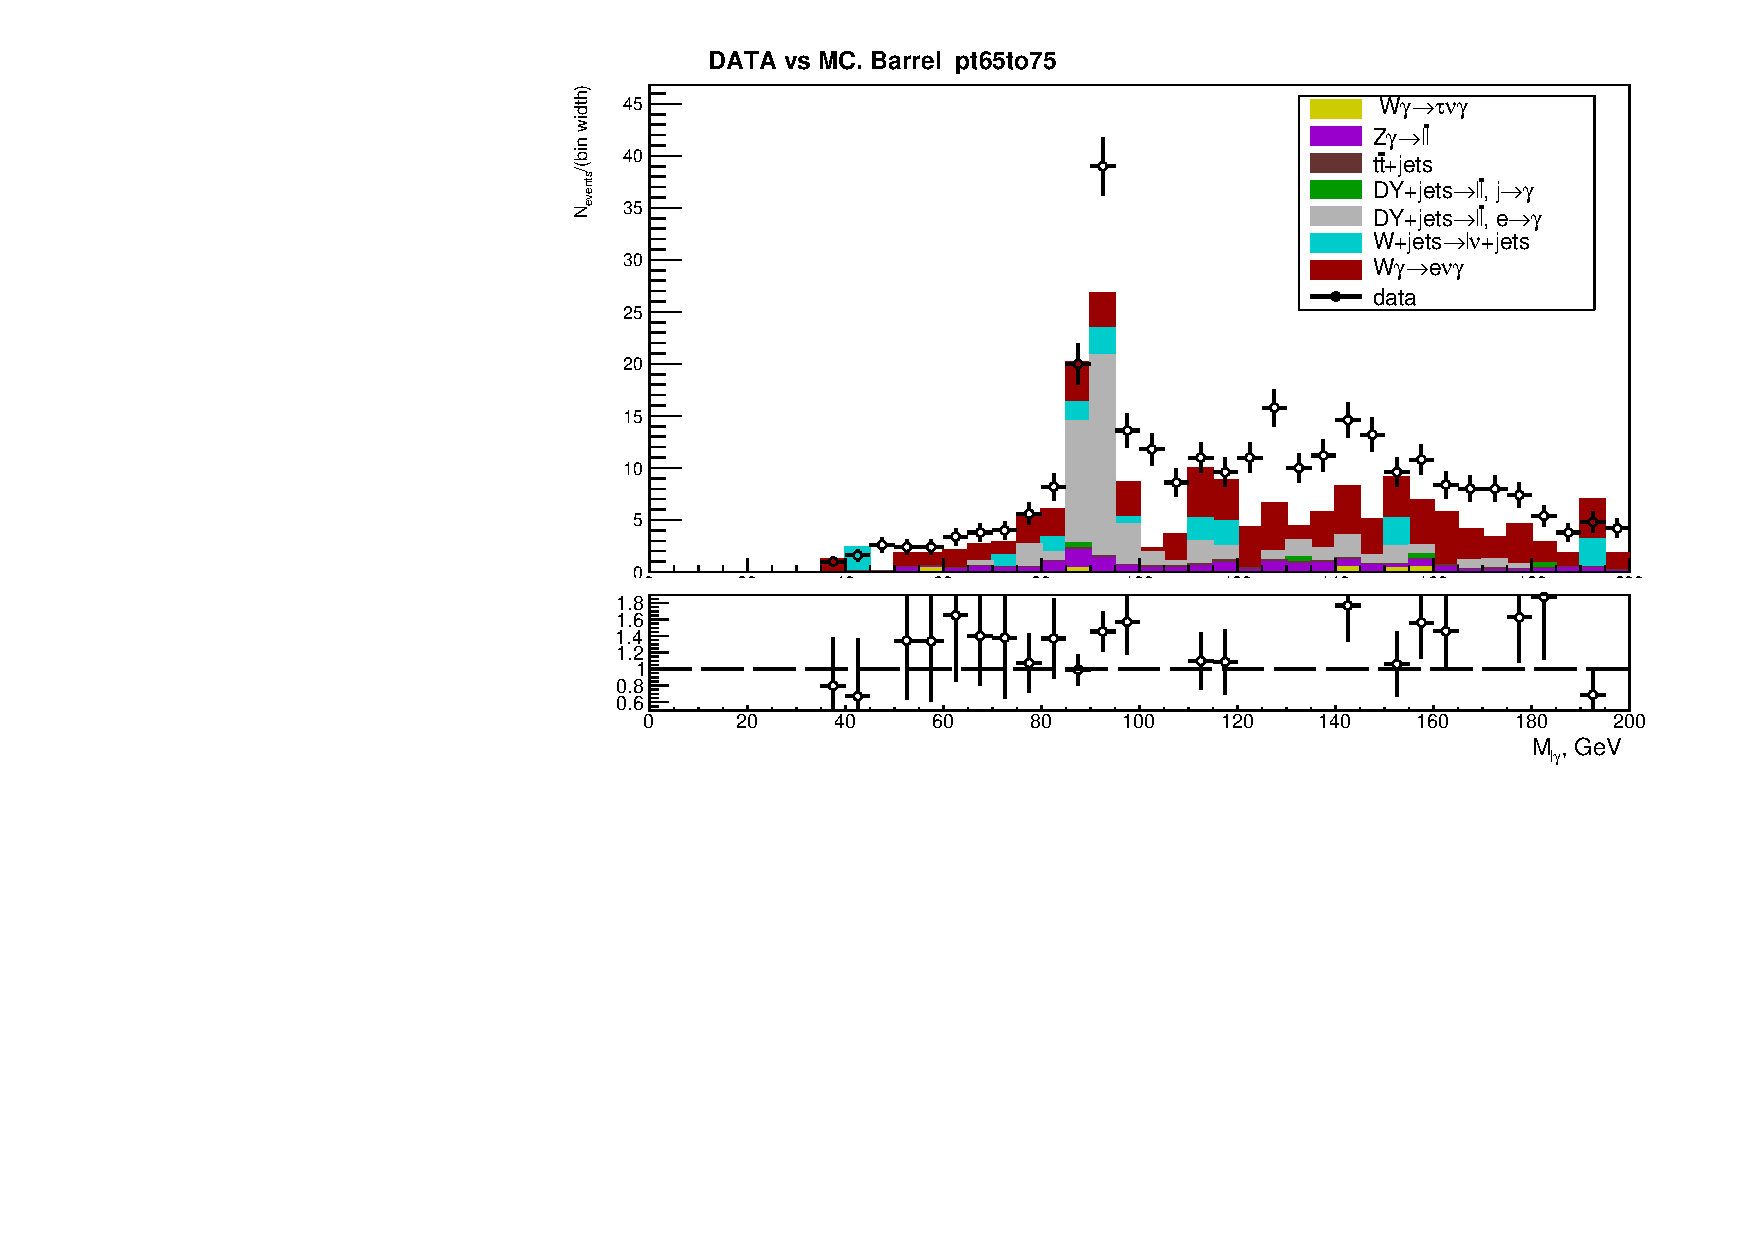
\includegraphics[width=0.40\textwidth]{../figs/figs_v11/ELECTRON_WGamma/PrepareYields/c_TotalDATAvsMC_Barrel__Mpholep1PRELIMINARY_FOR_E_TO_GAMMA_WITH_PSV_CUT_pt65to75_.pdf}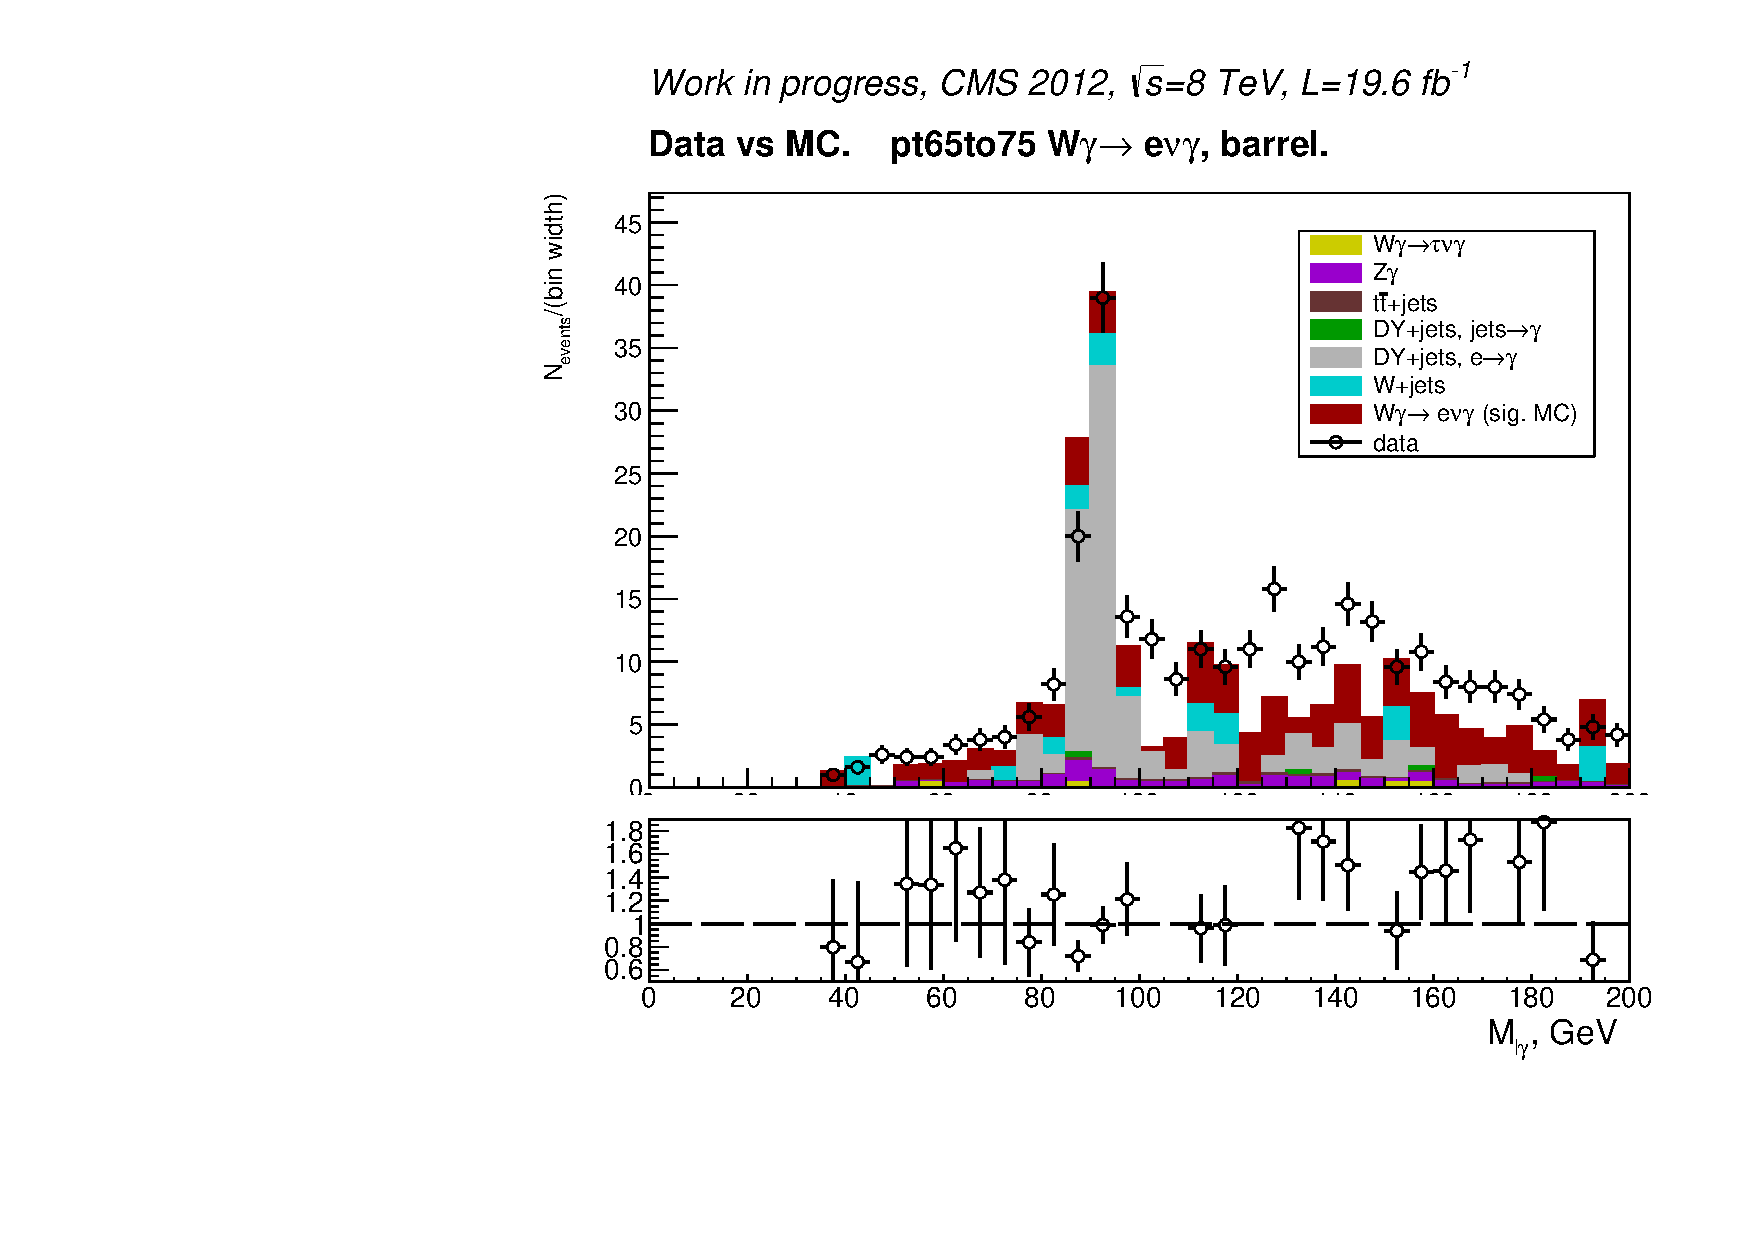
\includegraphics[width=0.40\textwidth]{../figs/figs_v11/ELECTRON_WGamma/PrepareYields/c_TotalDATAvsMC_Barrel__Mpholep1PRELIMINARY_FOR_E_TO_GAMMA_WITH_PSV_CUT_pt65to75__etogScale.pdf}\\
    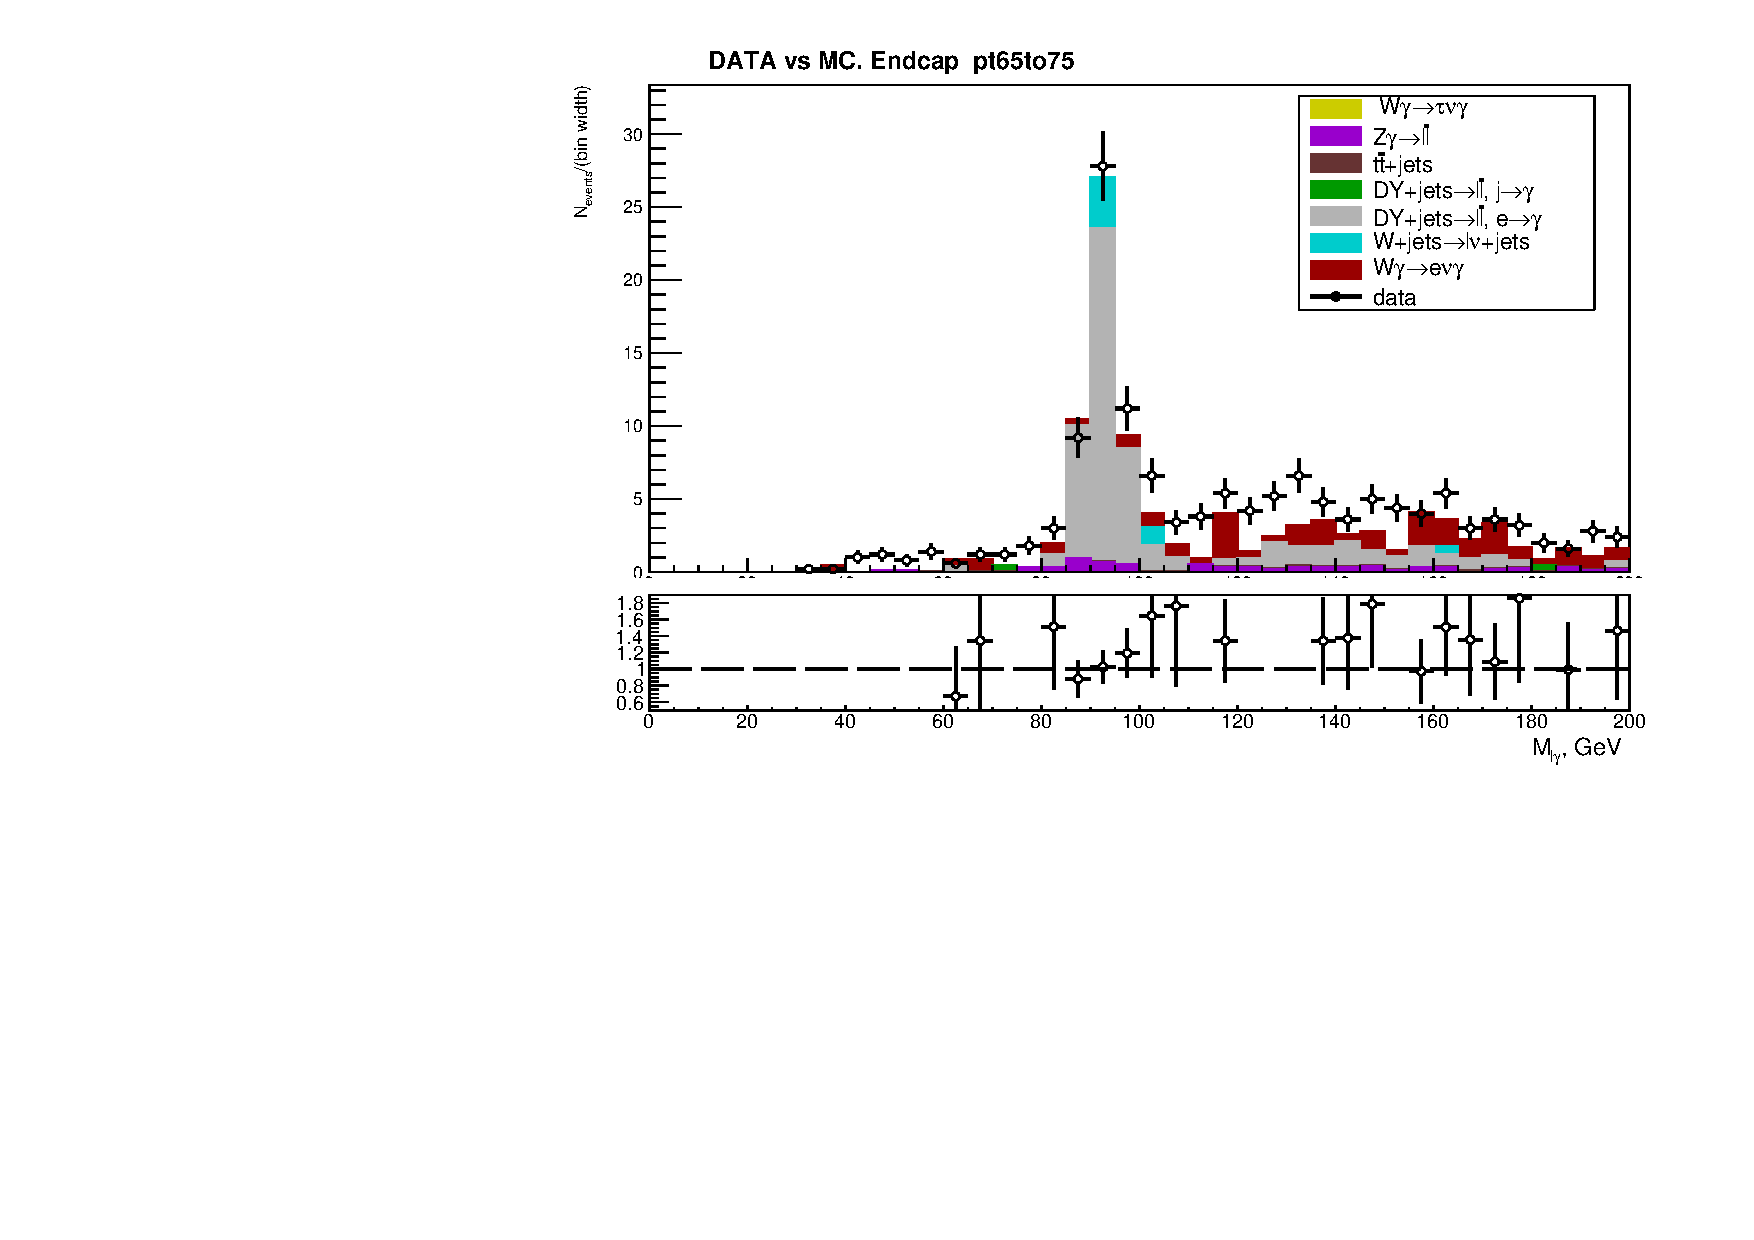
\includegraphics[width=0.40\textwidth]{../figs/figs_v11/ELECTRON_WGamma/PrepareYields/c_TotalDATAvsMC_Endcap__Mpholep1PRELIMINARY_FOR_E_TO_GAMMA_WITH_PSV_CUT_pt65to75_.pdf}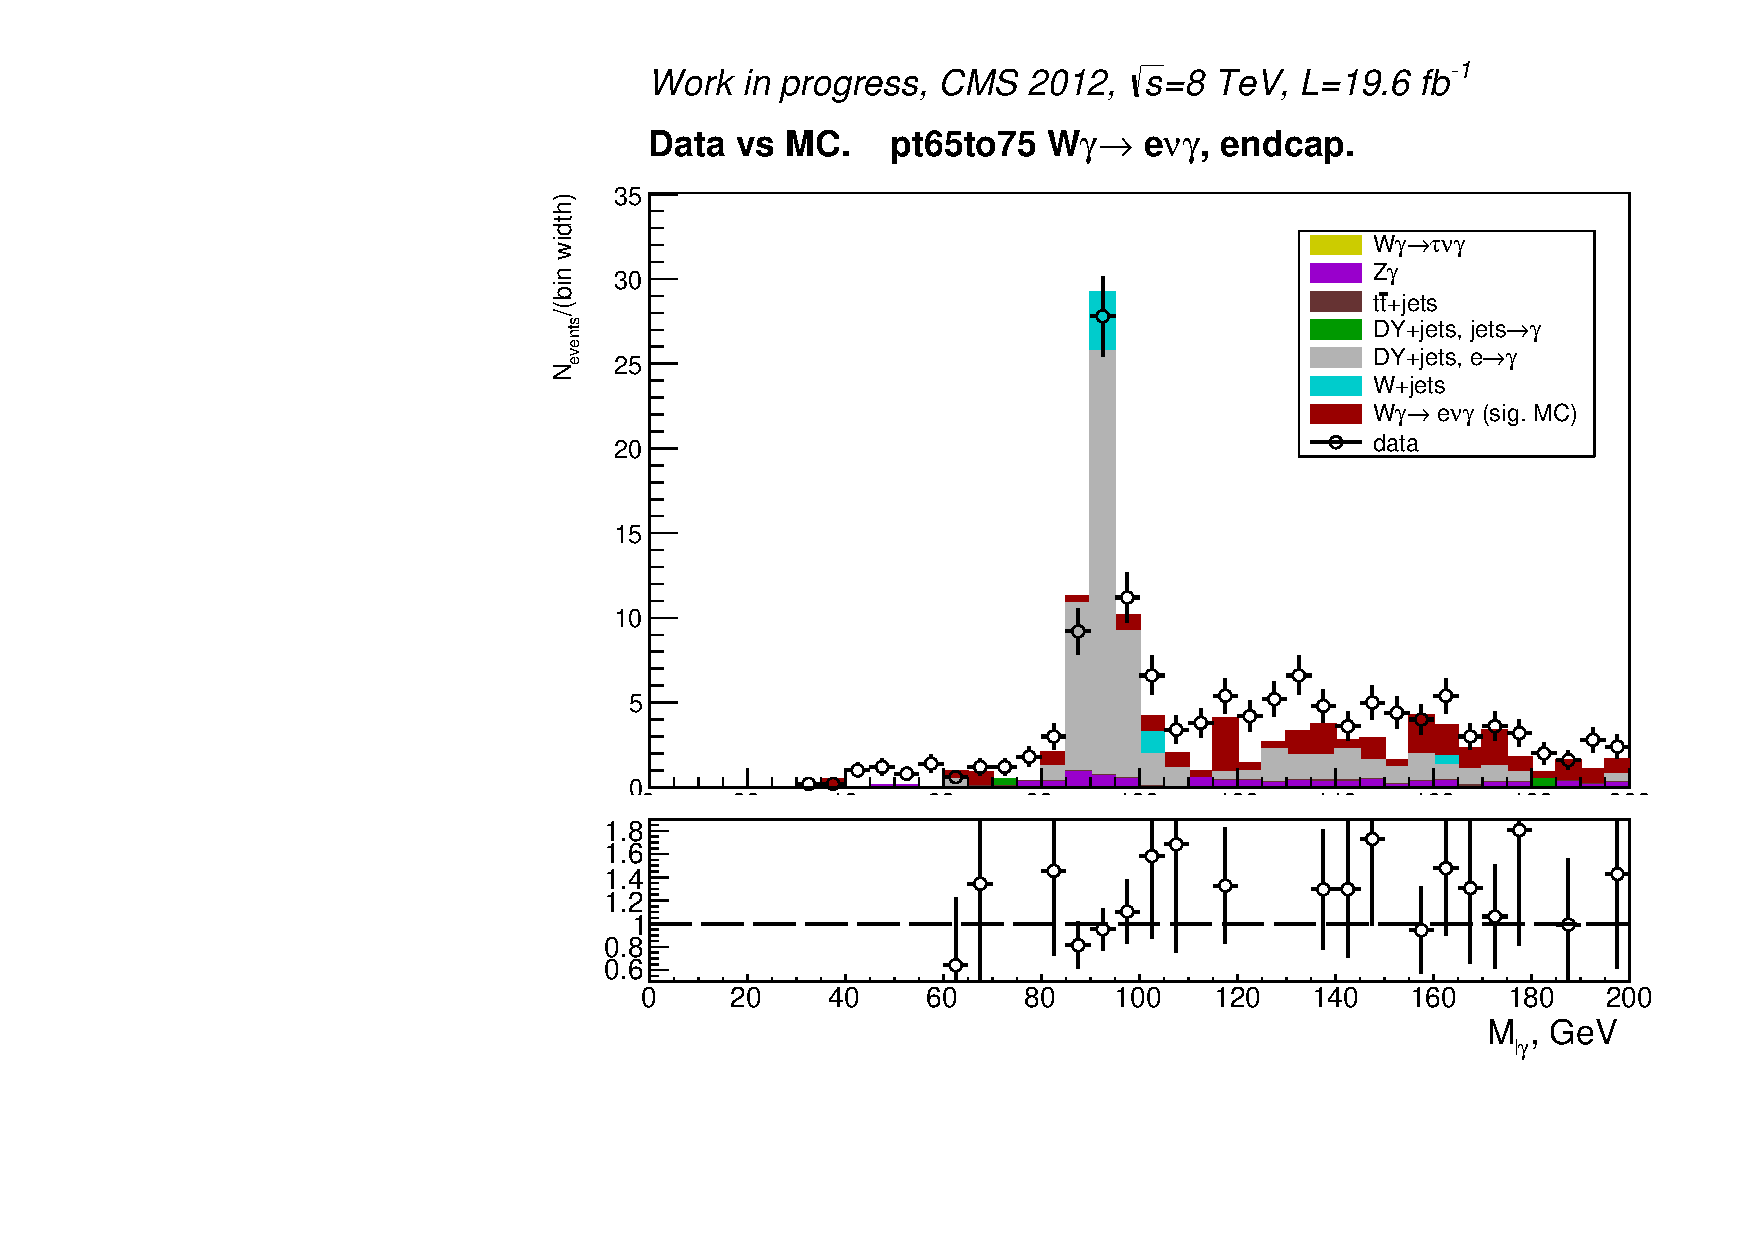
\includegraphics[width=0.40\textwidth]{../figs/figs_v11/ELECTRON_WGamma/PrepareYields/c_TotalDATAvsMC_Endcap__Mpholep1PRELIMINARY_FOR_E_TO_GAMMA_WITH_PSV_CUT_pt65to75__etogScale.pdf}\\
   \label{fig:Mpholep1DatavsMC_35to75}
  \caption{$M_{e,\gamma}$ distribution, data vs MC. Bins 55-65-75 GeV. Left: all MC samples are normalized to luminocity of data, PU weight adn SFs, right: DY$\rightarrow$jets(e$\rightarrow\gamma$) also normalized to e$\rightarrow\gamma$ data-driven estimates.}
  \end{center}
\end{figure}

\begin{figure}[htb]
  \begin{center}
    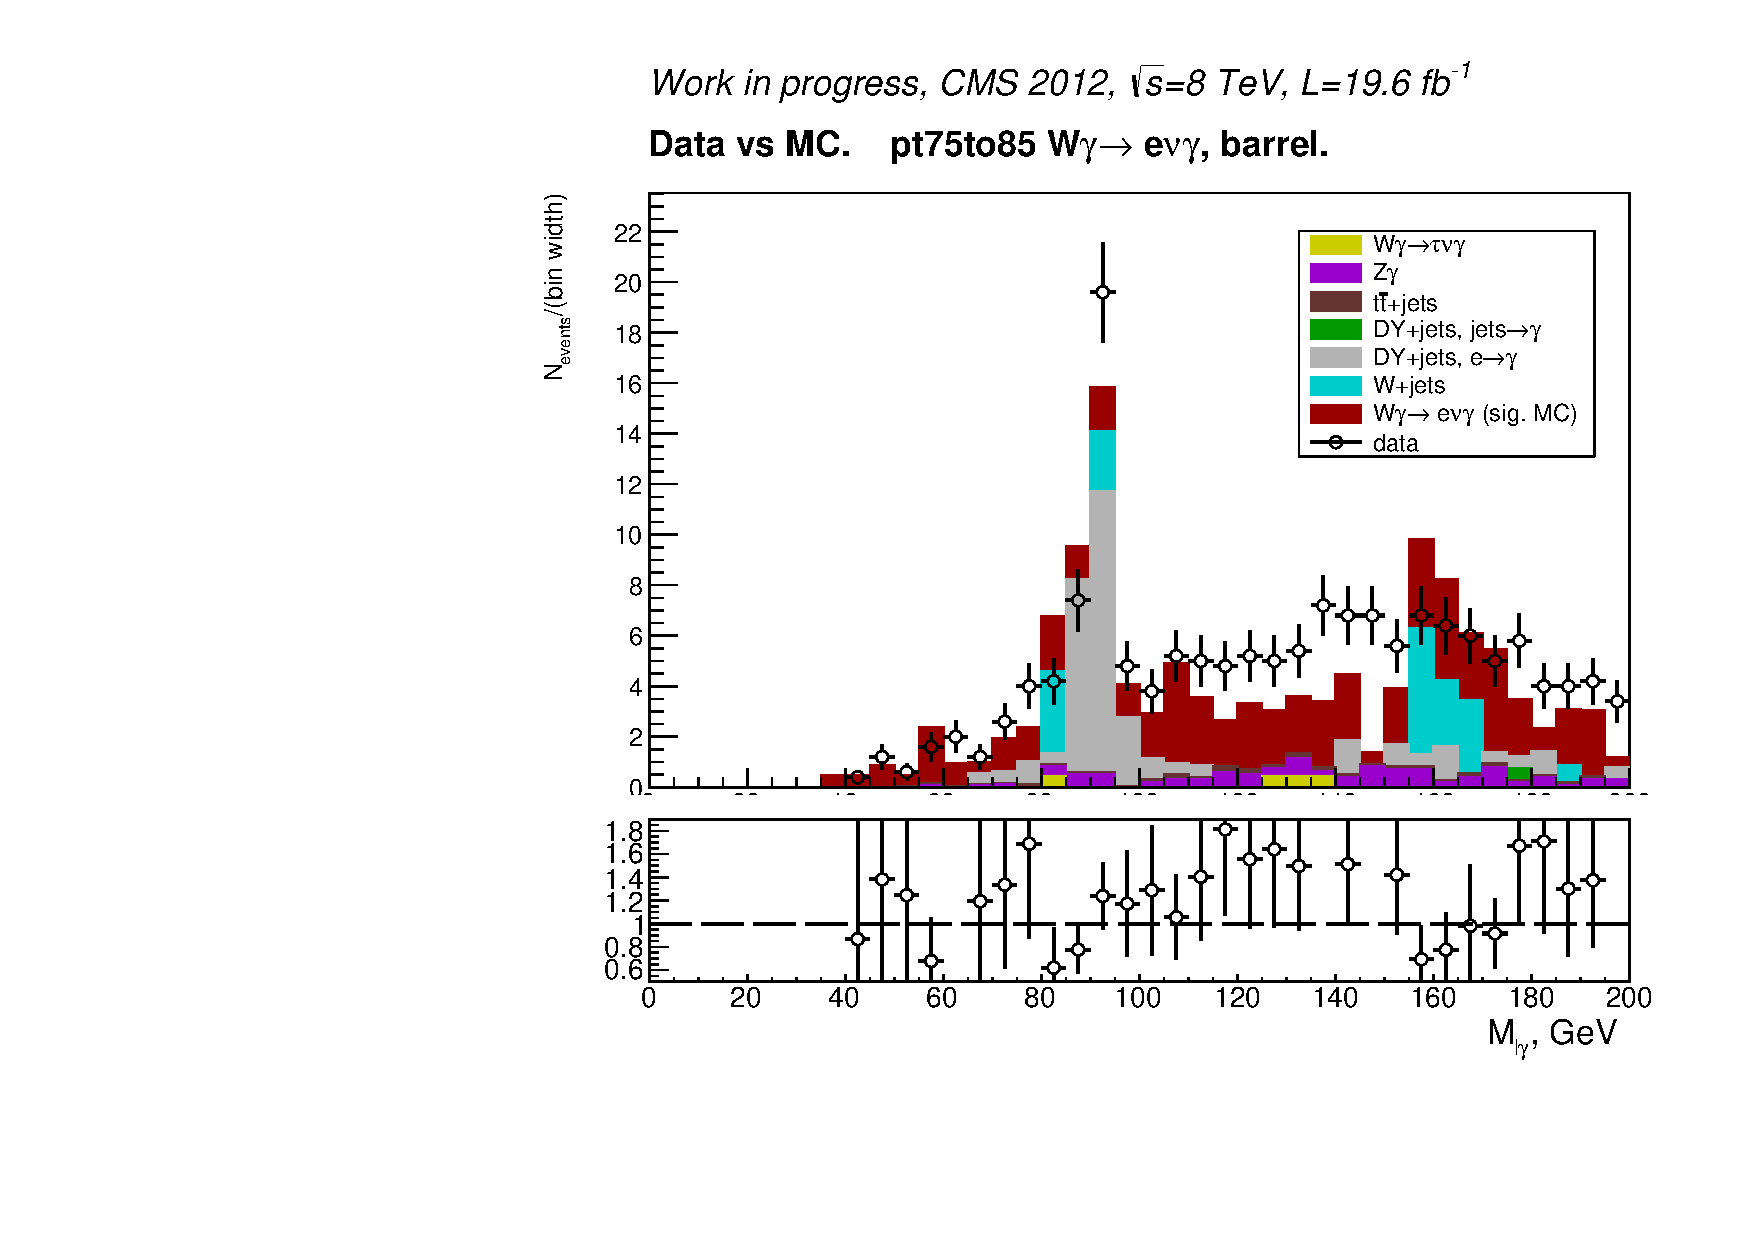
\includegraphics[width=0.40\textwidth]{../figs/figs_v11/ELECTRON_WGamma/PrepareYields/c_TotalDATAvsMC_Barrel__Mpholep1PRELIMINARY_FOR_E_TO_GAMMA_WITH_PSV_CUT_pt75to85_.pdf}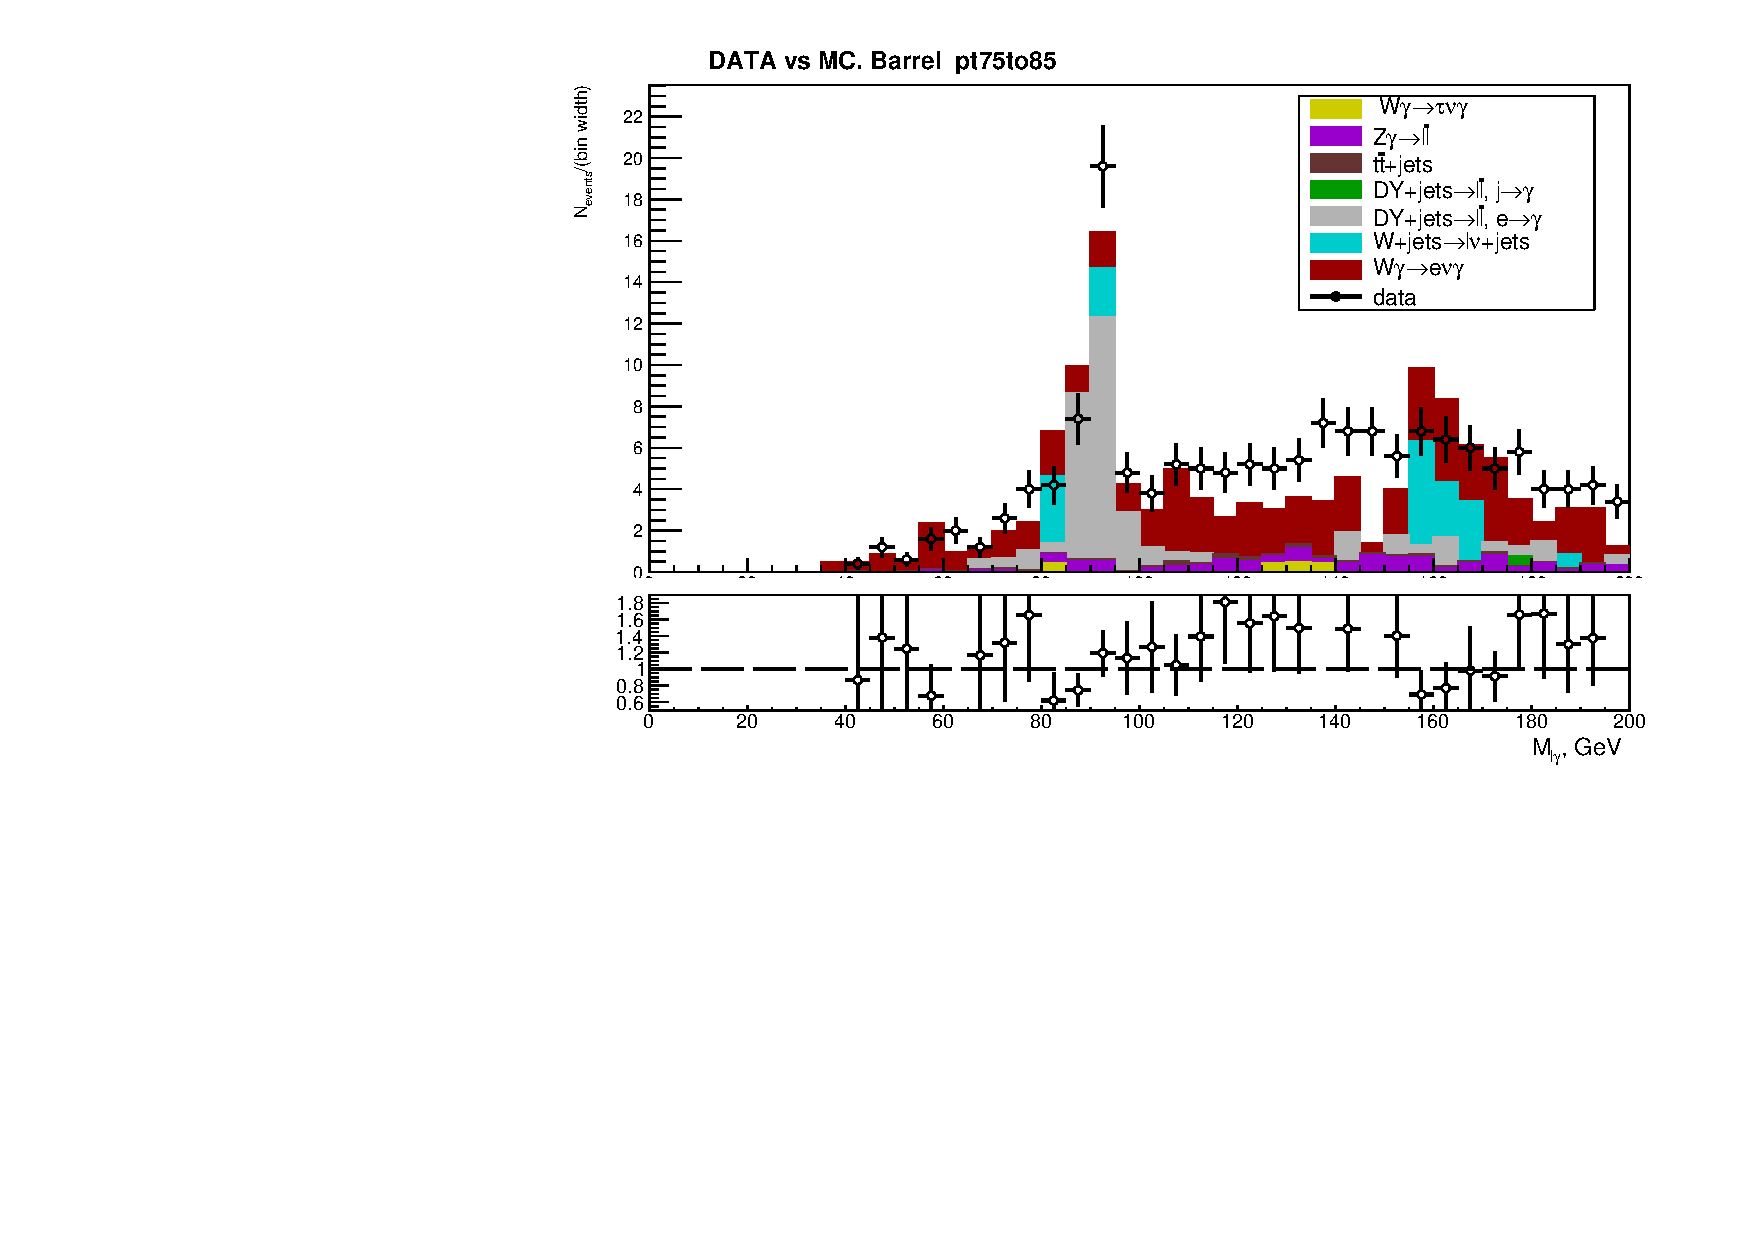
\includegraphics[width=0.40\textwidth]{../figs/figs_v11/ELECTRON_WGamma/PrepareYields/c_TotalDATAvsMC_Barrel__Mpholep1PRELIMINARY_FOR_E_TO_GAMMA_WITH_PSV_CUT_pt75to85__etogScale.pdf}\\
    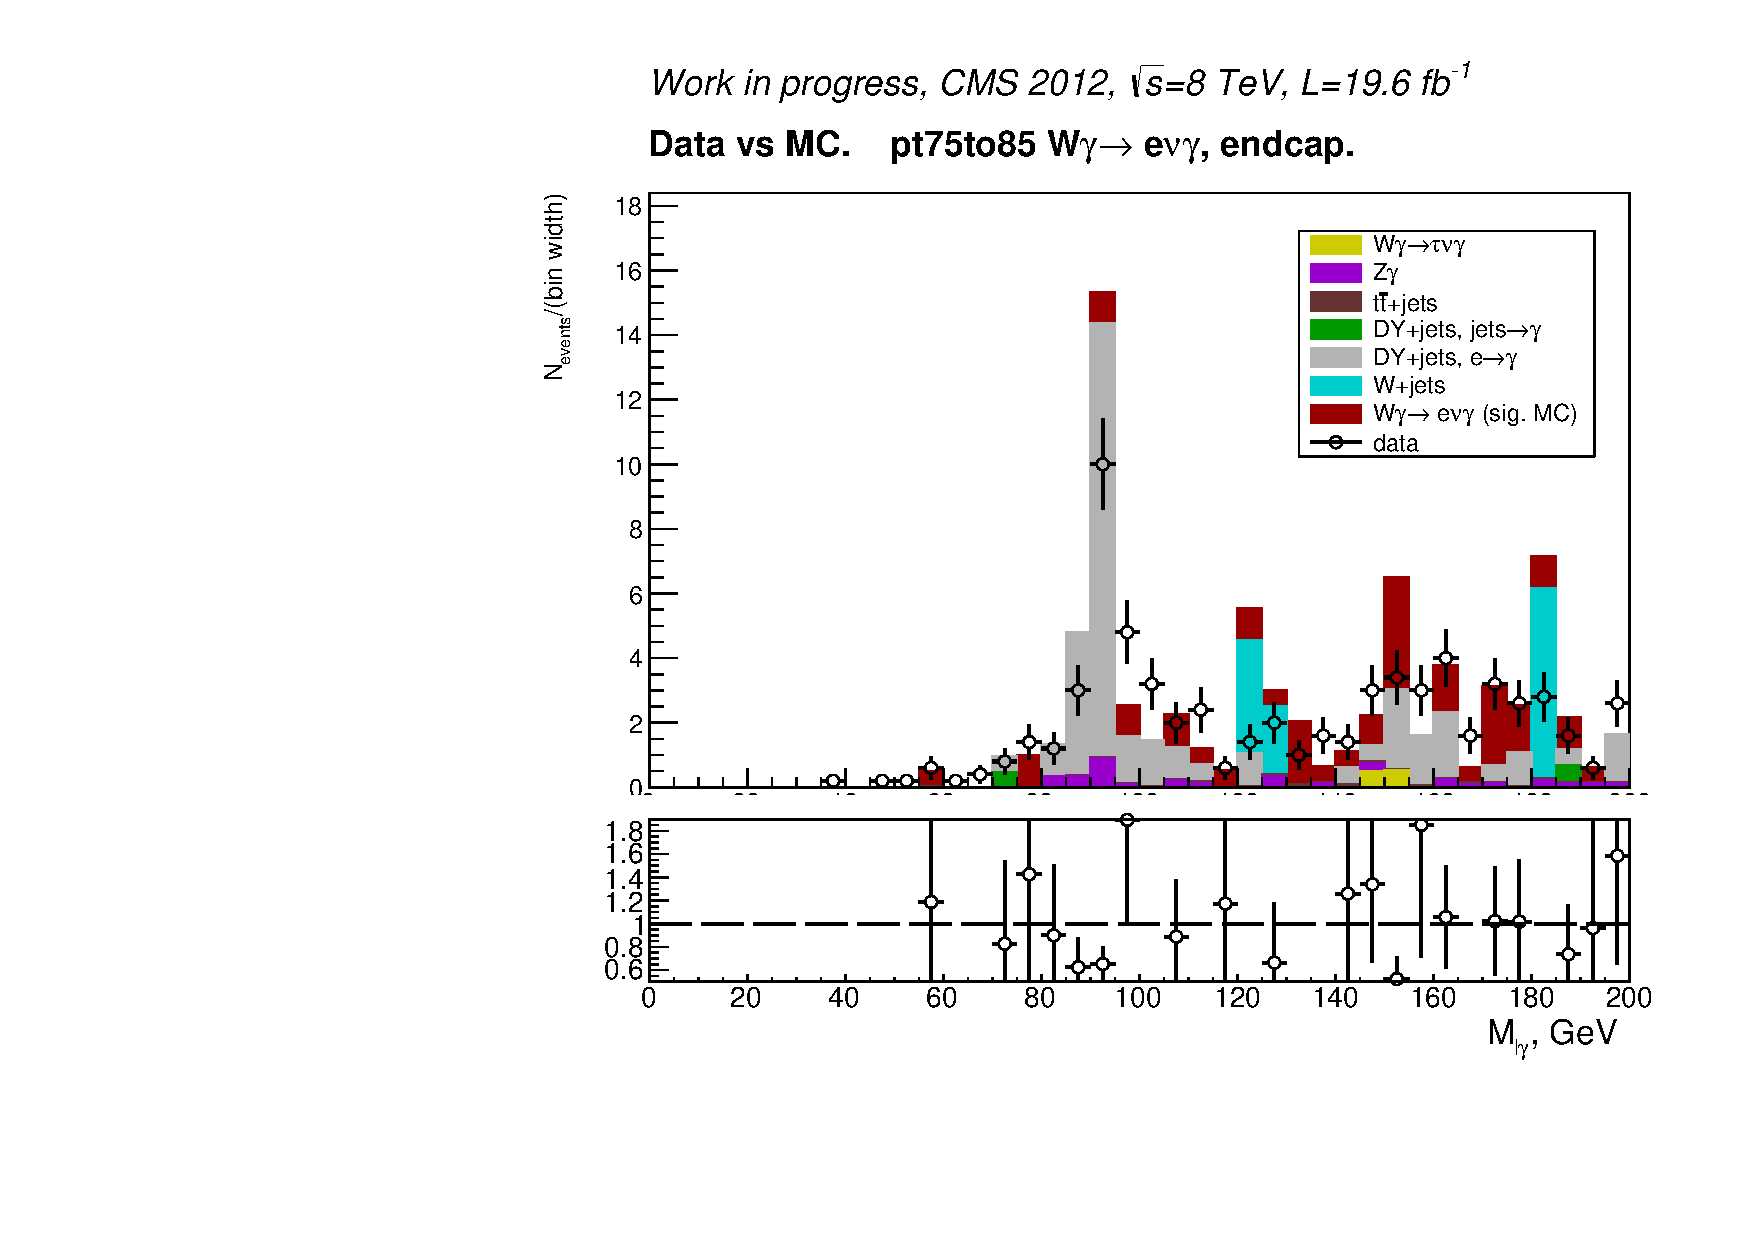
\includegraphics[width=0.40\textwidth]{../figs/figs_v11/ELECTRON_WGamma/PrepareYields/c_TotalDATAvsMC_Endcap__Mpholep1PRELIMINARY_FOR_E_TO_GAMMA_WITH_PSV_CUT_pt75to85_.pdf}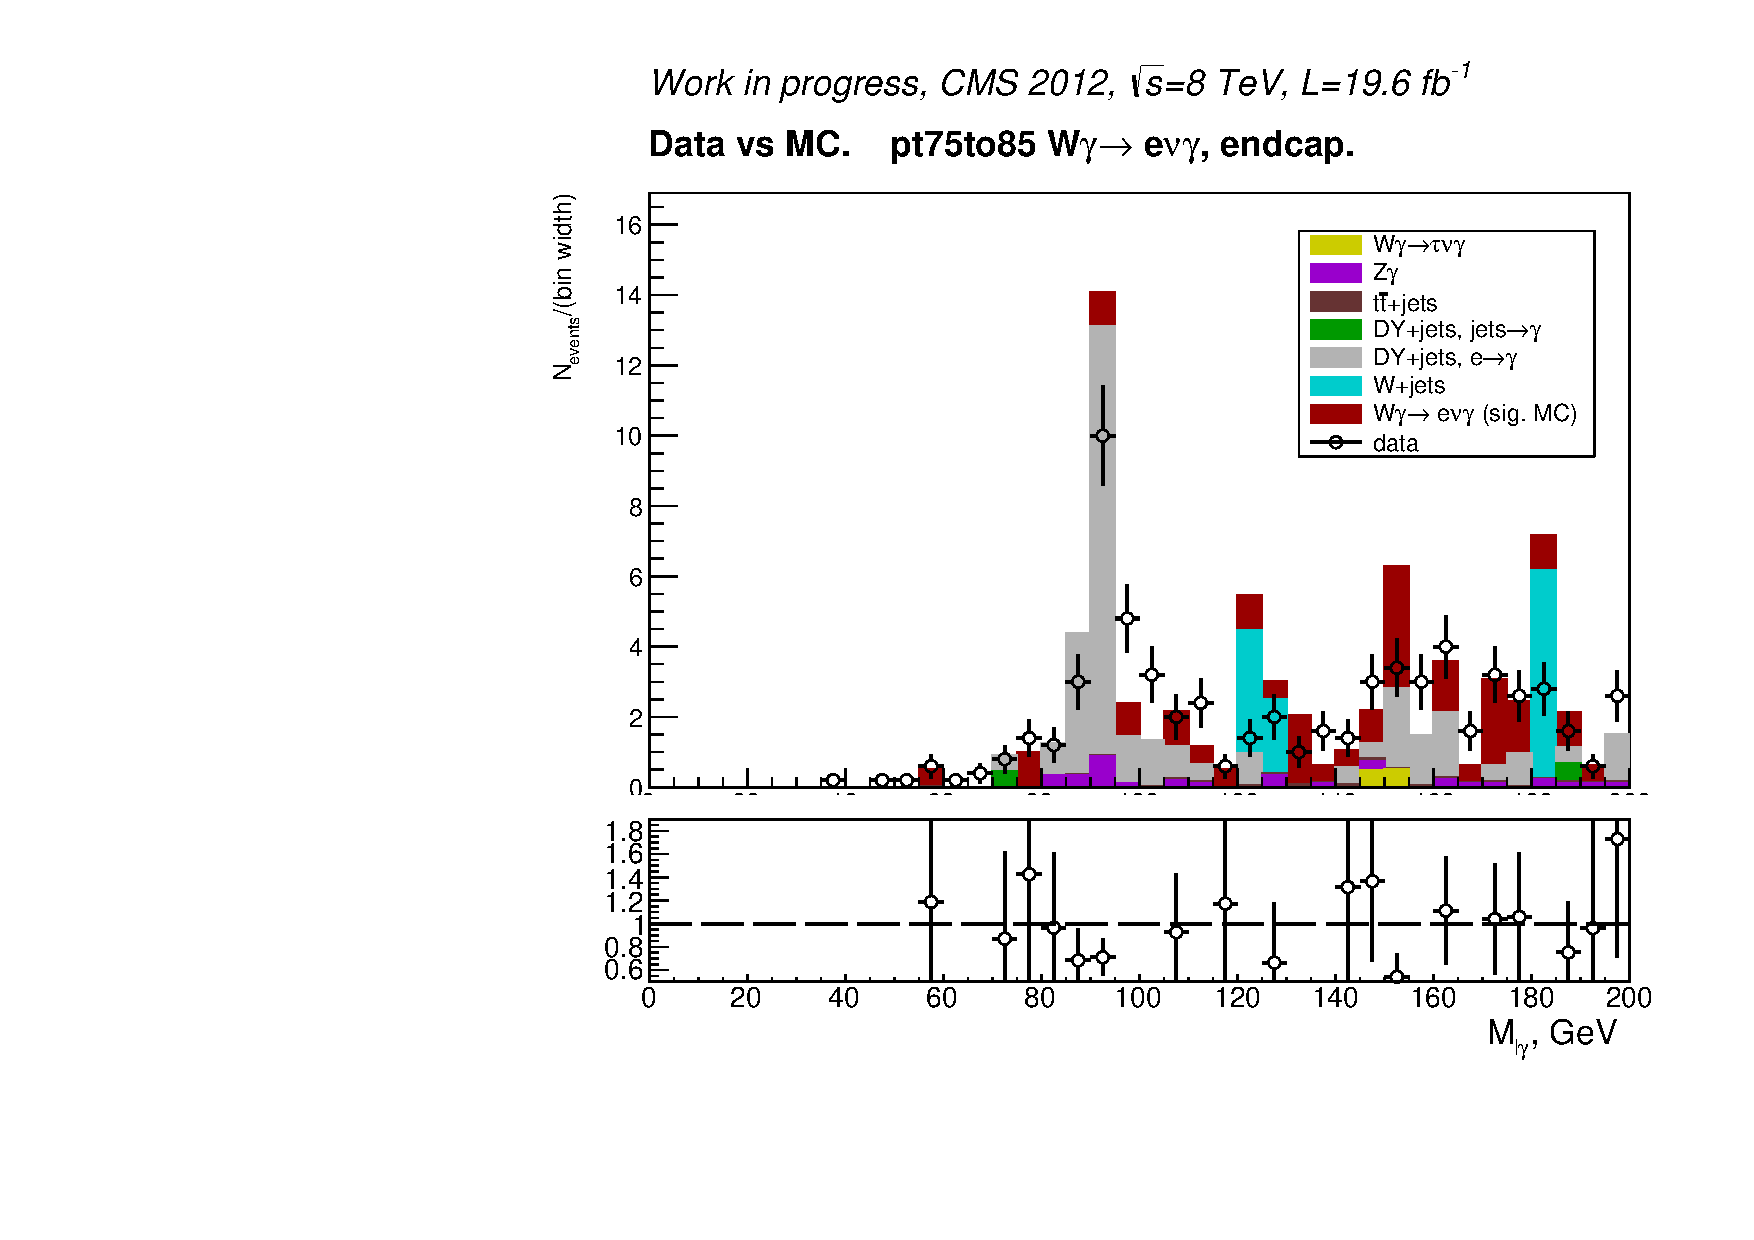
\includegraphics[width=0.40\textwidth]{../figs/figs_v11/ELECTRON_WGamma/PrepareYields/c_TotalDATAvsMC_Endcap__Mpholep1PRELIMINARY_FOR_E_TO_GAMMA_WITH_PSV_CUT_pt75to85__etogScale.pdf}\\
    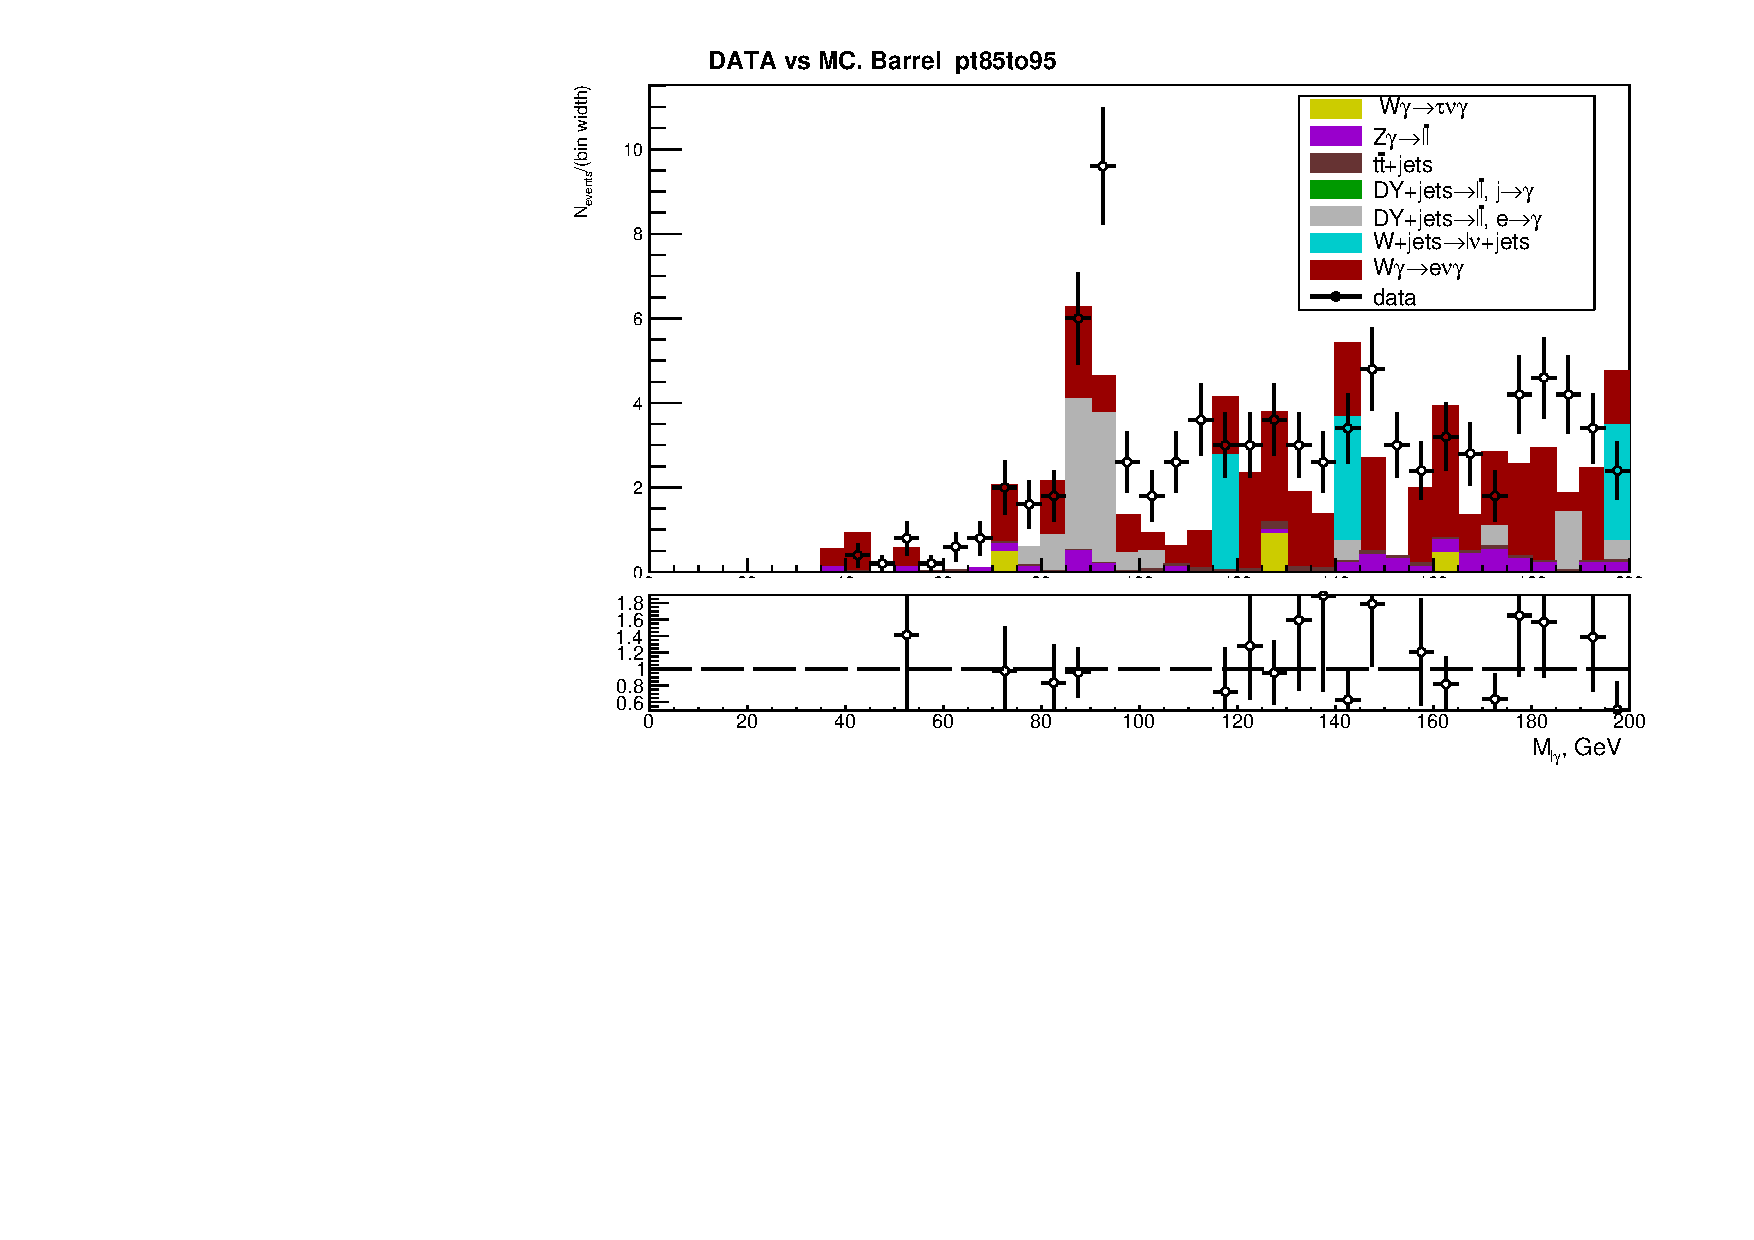
\includegraphics[width=0.40\textwidth]{../figs/figs_v11/ELECTRON_WGamma/PrepareYields/c_TotalDATAvsMC_Barrel__Mpholep1PRELIMINARY_FOR_E_TO_GAMMA_WITH_PSV_CUT_pt85to95_.pdf}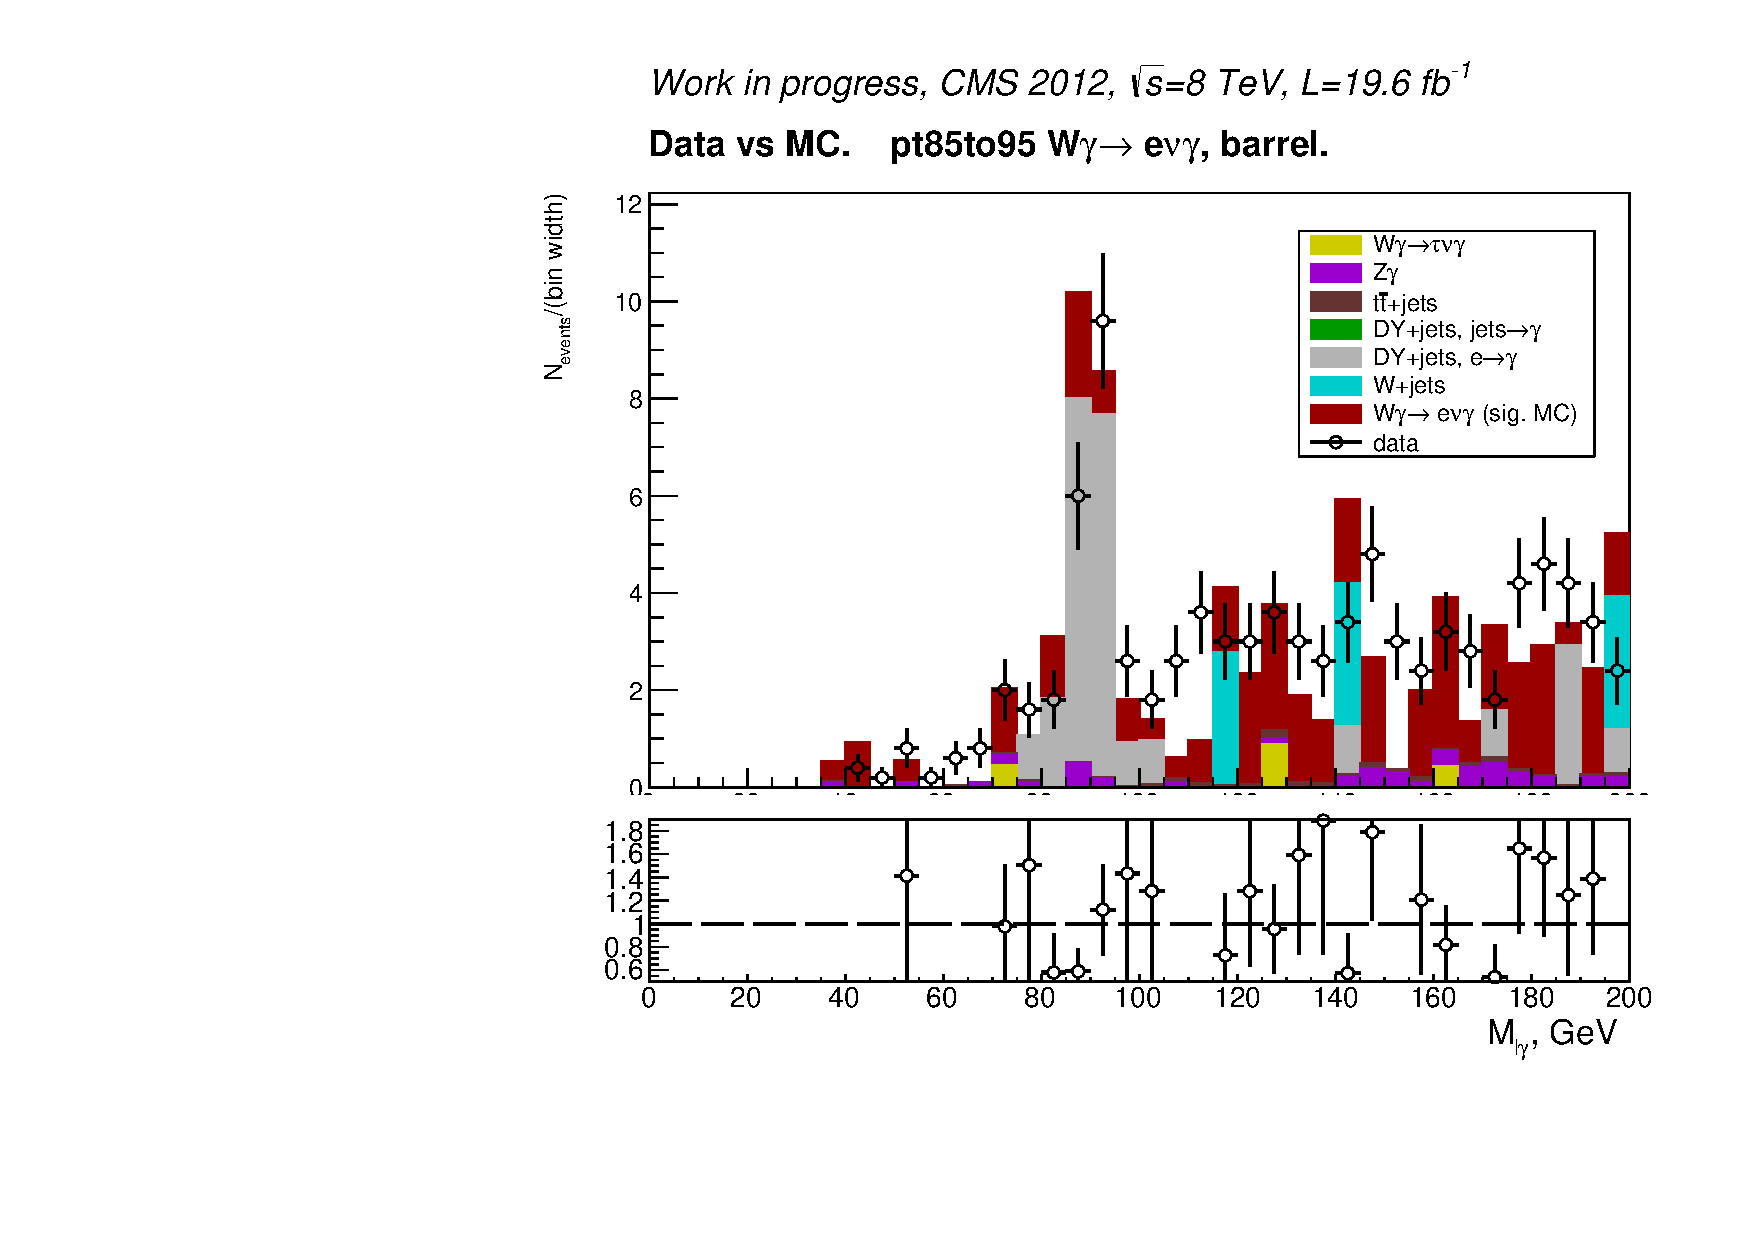
\includegraphics[width=0.40\textwidth]{../figs/figs_v11/ELECTRON_WGamma/PrepareYields/c_TotalDATAvsMC_Barrel__Mpholep1PRELIMINARY_FOR_E_TO_GAMMA_WITH_PSV_CUT_pt85to95__etogScale.pdf}\\ 
    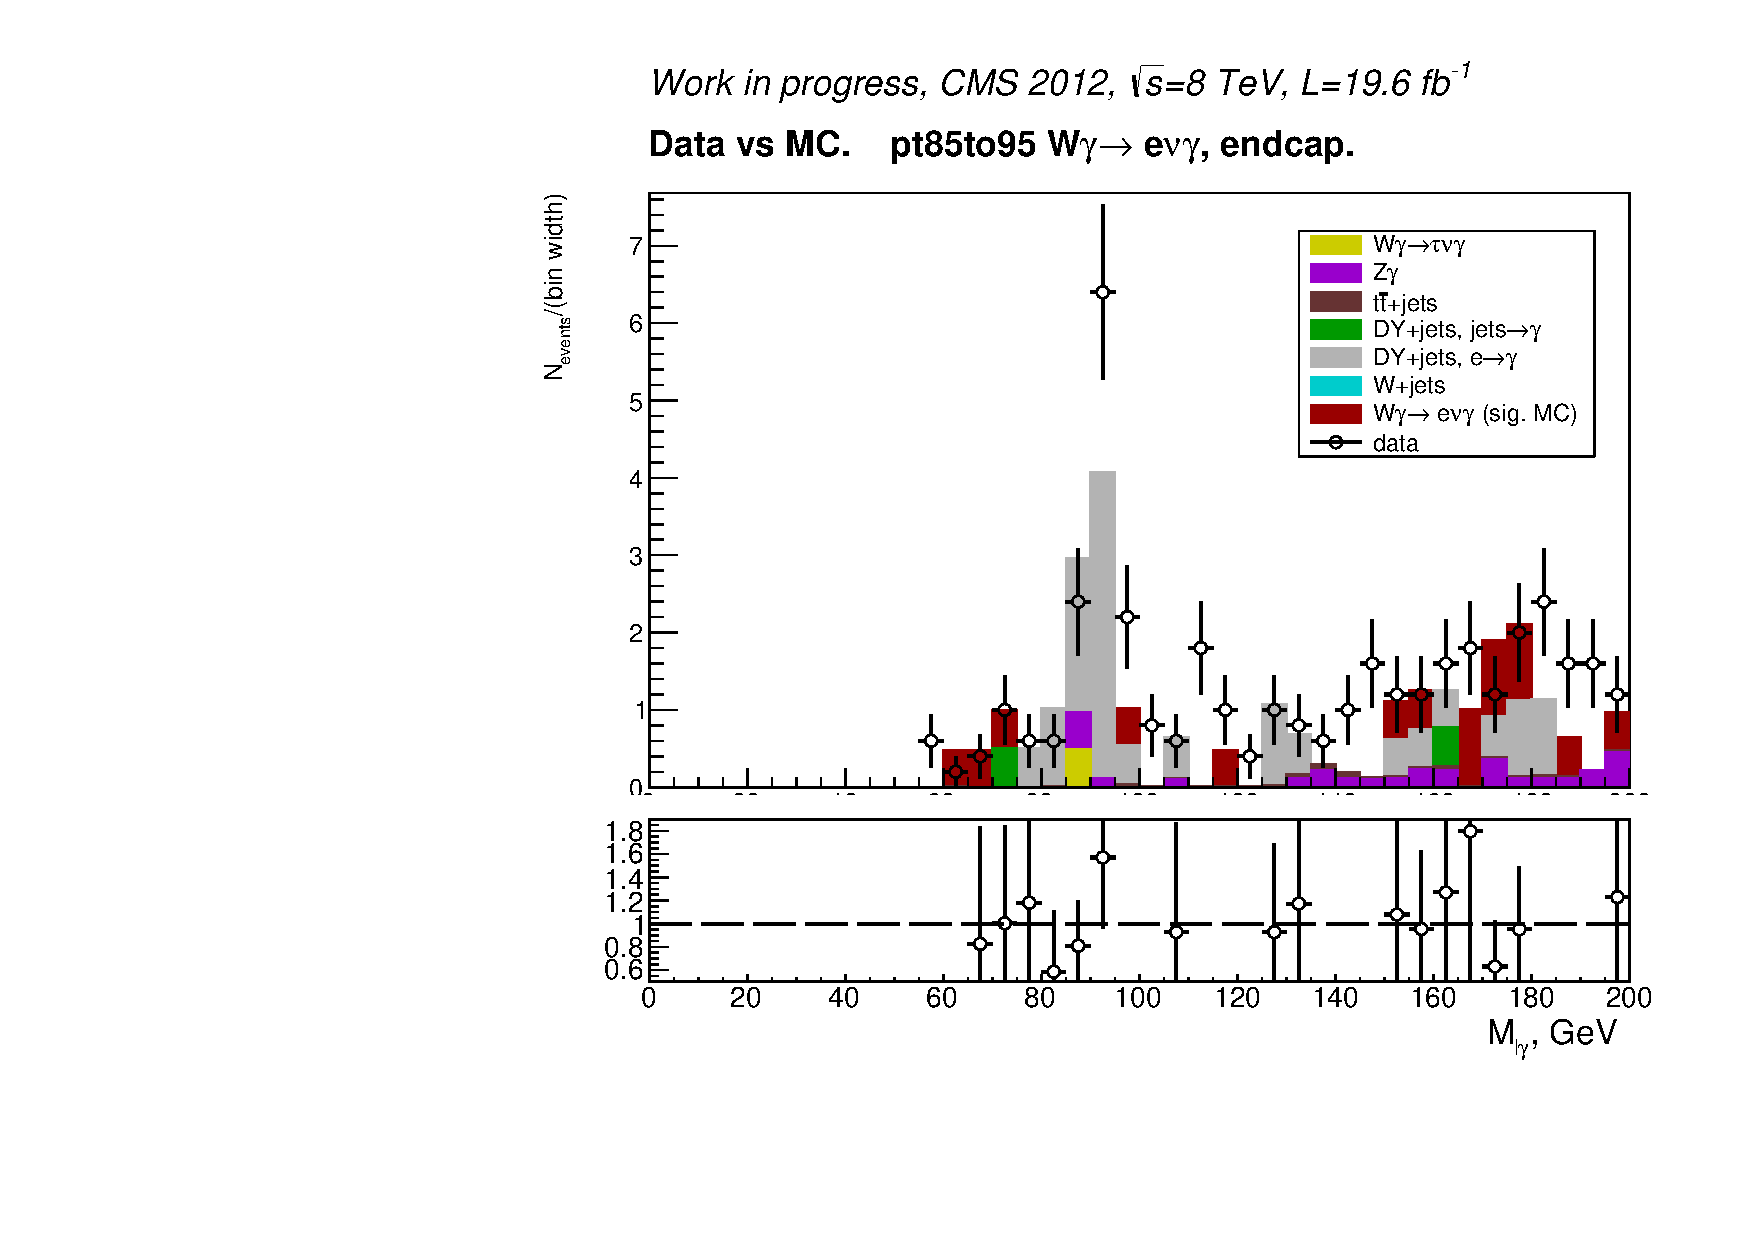
\includegraphics[width=0.40\textwidth]{../figs/figs_v11/ELECTRON_WGamma/PrepareYields/c_TotalDATAvsMC_Endcap__Mpholep1PRELIMINARY_FOR_E_TO_GAMMA_WITH_PSV_CUT_pt85to95_.pdf}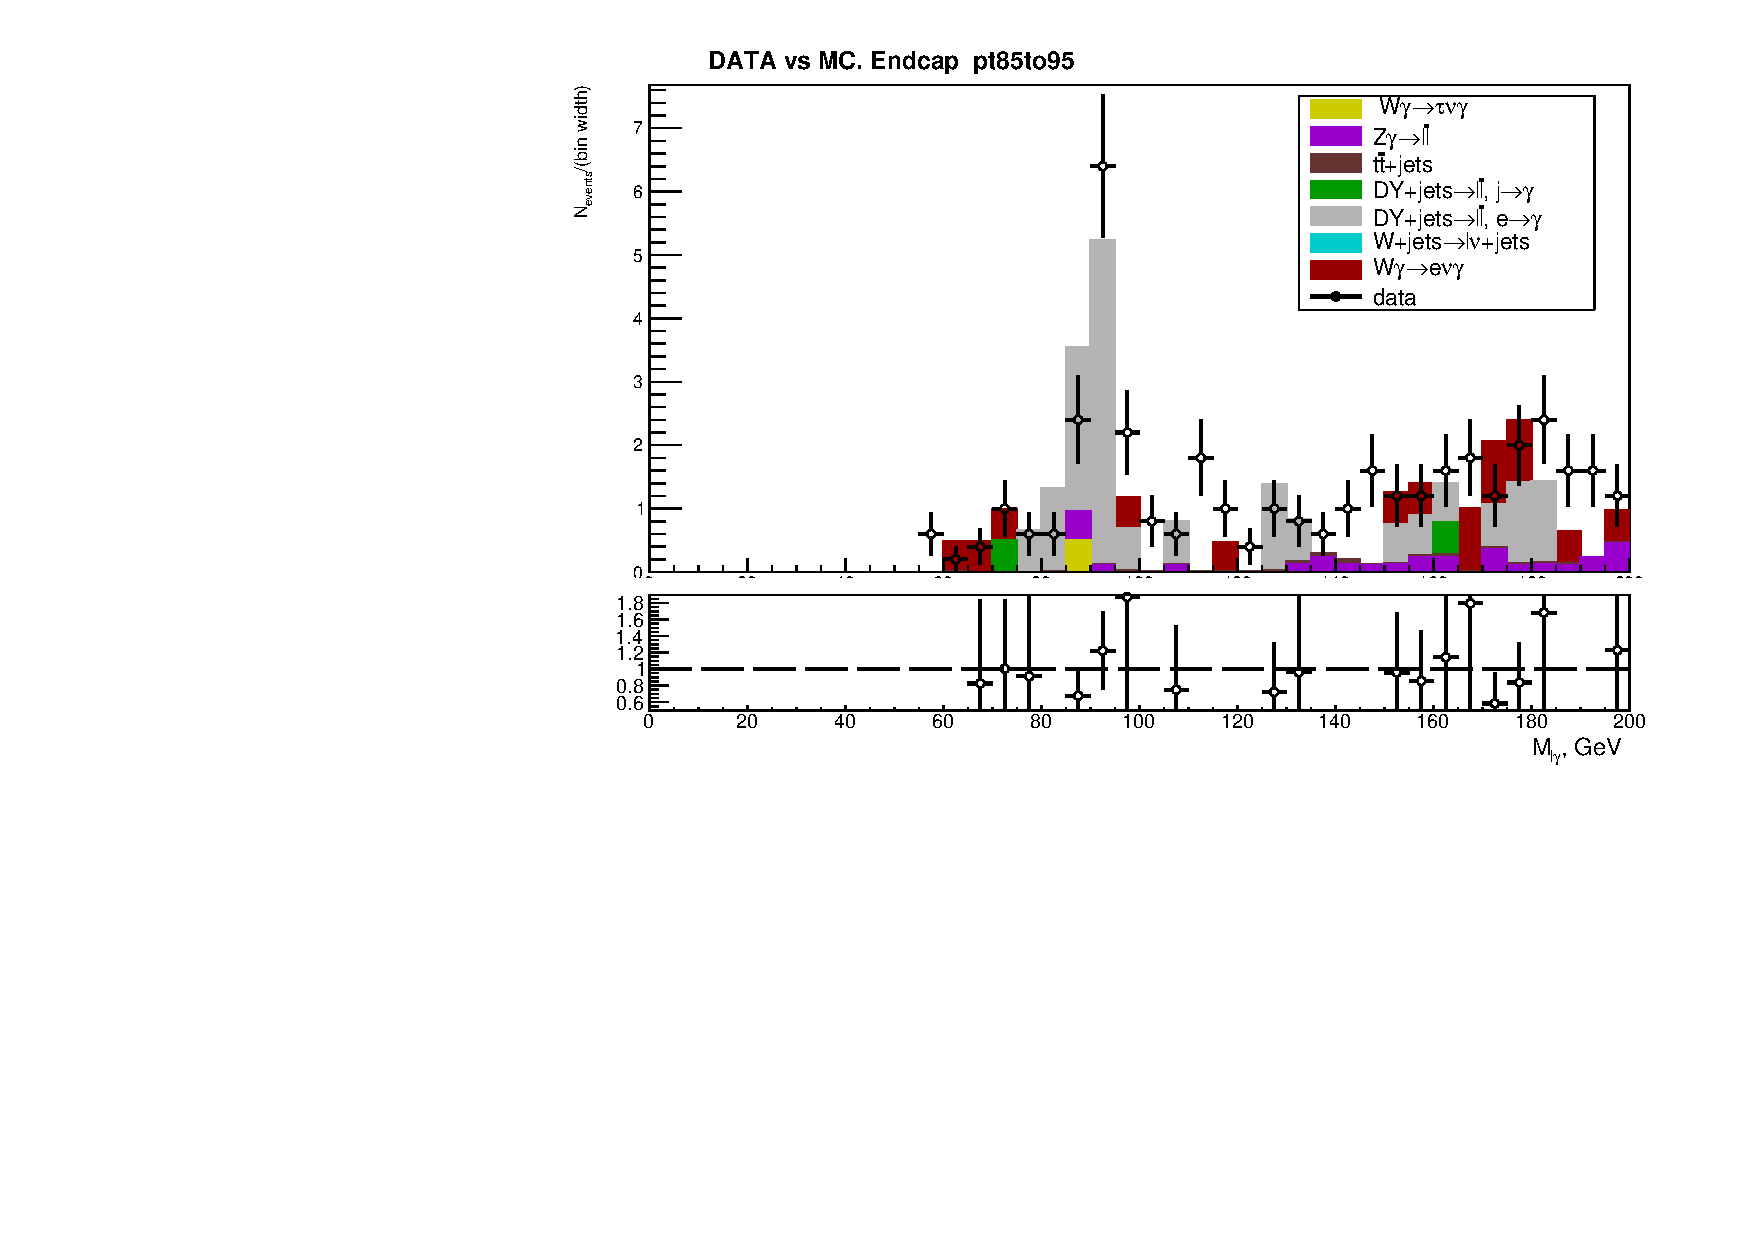
\includegraphics[width=0.40\textwidth]{../figs/figs_v11/ELECTRON_WGamma/PrepareYields/c_TotalDATAvsMC_Endcap__Mpholep1PRELIMINARY_FOR_E_TO_GAMMA_WITH_PSV_CUT_pt85to95__etogScale.pdf}\\
   \label{fig:Mpholep1DatavsMC_75to500}
  \caption{$M_{e,\gamma}$ distribution, data vs MC. Bins 75-85-95 GeV. Left: all MC samples are normalized to luminocity of data, PU weight adn SFs, right: DY$\rightarrow$jets(e$\rightarrow\gamma$) also normalized to e$\rightarrow\gamma$ data-driven estimates.}
  \end{center}
\end{figure}

\begin{figure}[htb]
  \begin{center}
    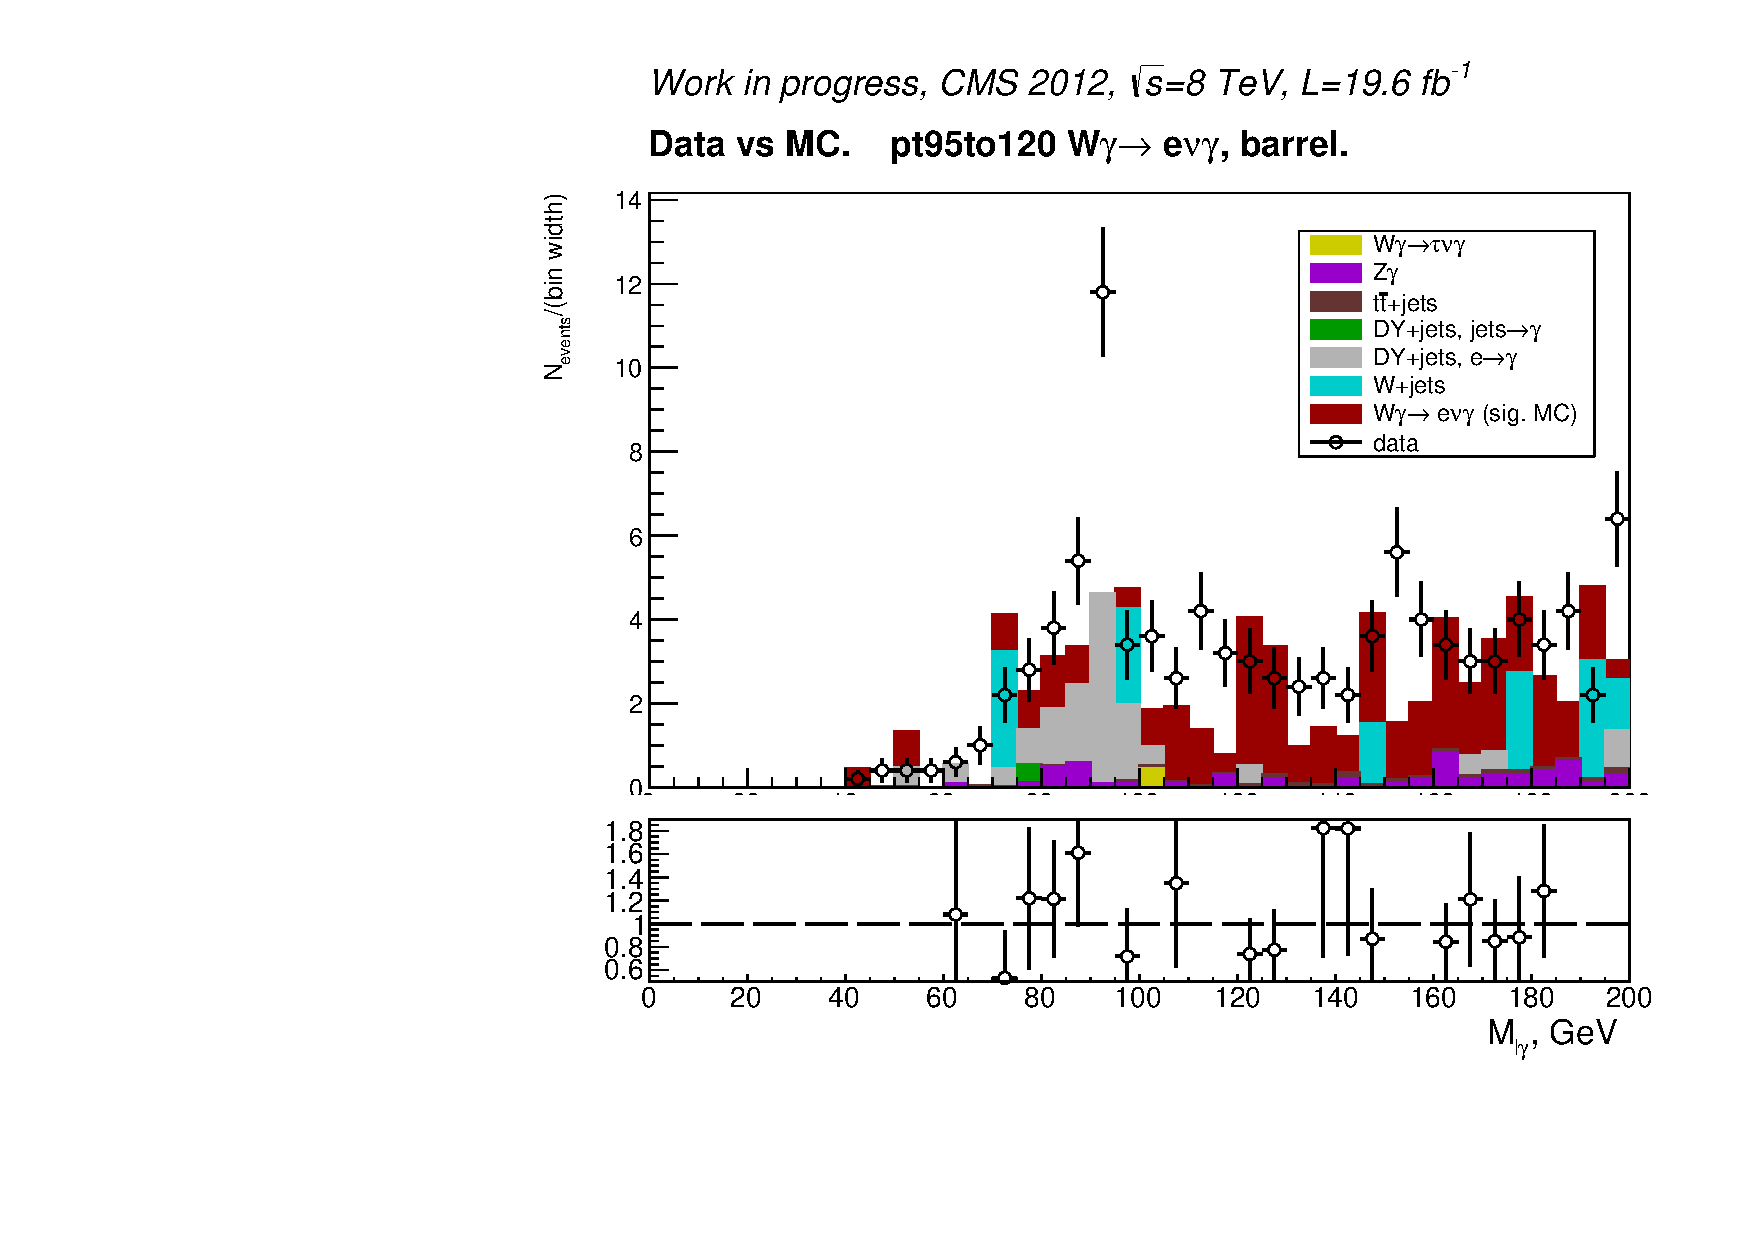
\includegraphics[width=0.40\textwidth]{../figs/figs_v11/ELECTRON_WGamma/PrepareYields/c_TotalDATAvsMC_Barrel__Mpholep1PRELIMINARY_FOR_E_TO_GAMMA_WITH_PSV_CUT_pt95to120_.pdf}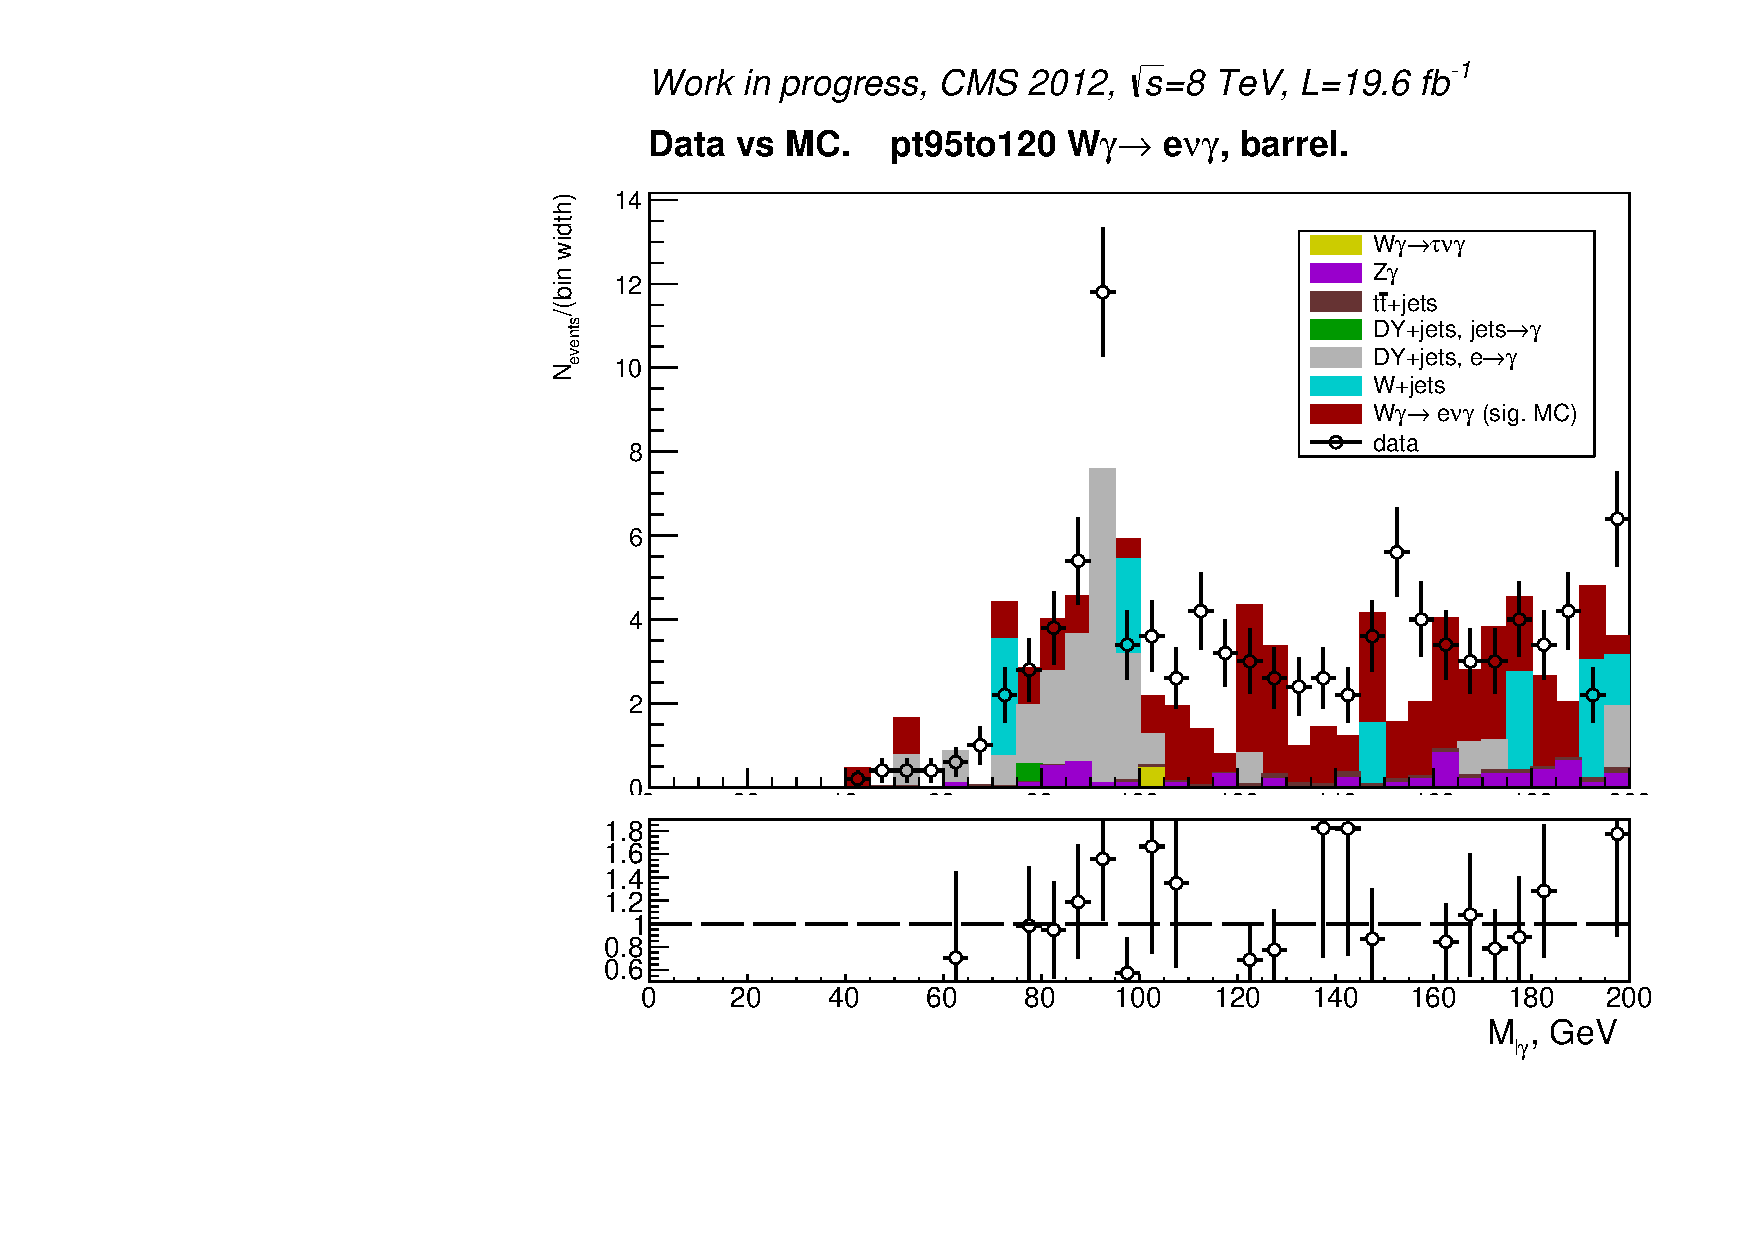
\includegraphics[width=0.40\textwidth]{../figs/figs_v11/ELECTRON_WGamma/PrepareYields/c_TotalDATAvsMC_Barrel__Mpholep1PRELIMINARY_FOR_E_TO_GAMMA_WITH_PSV_CUT_pt95to120__etogScale.pdf}\\
    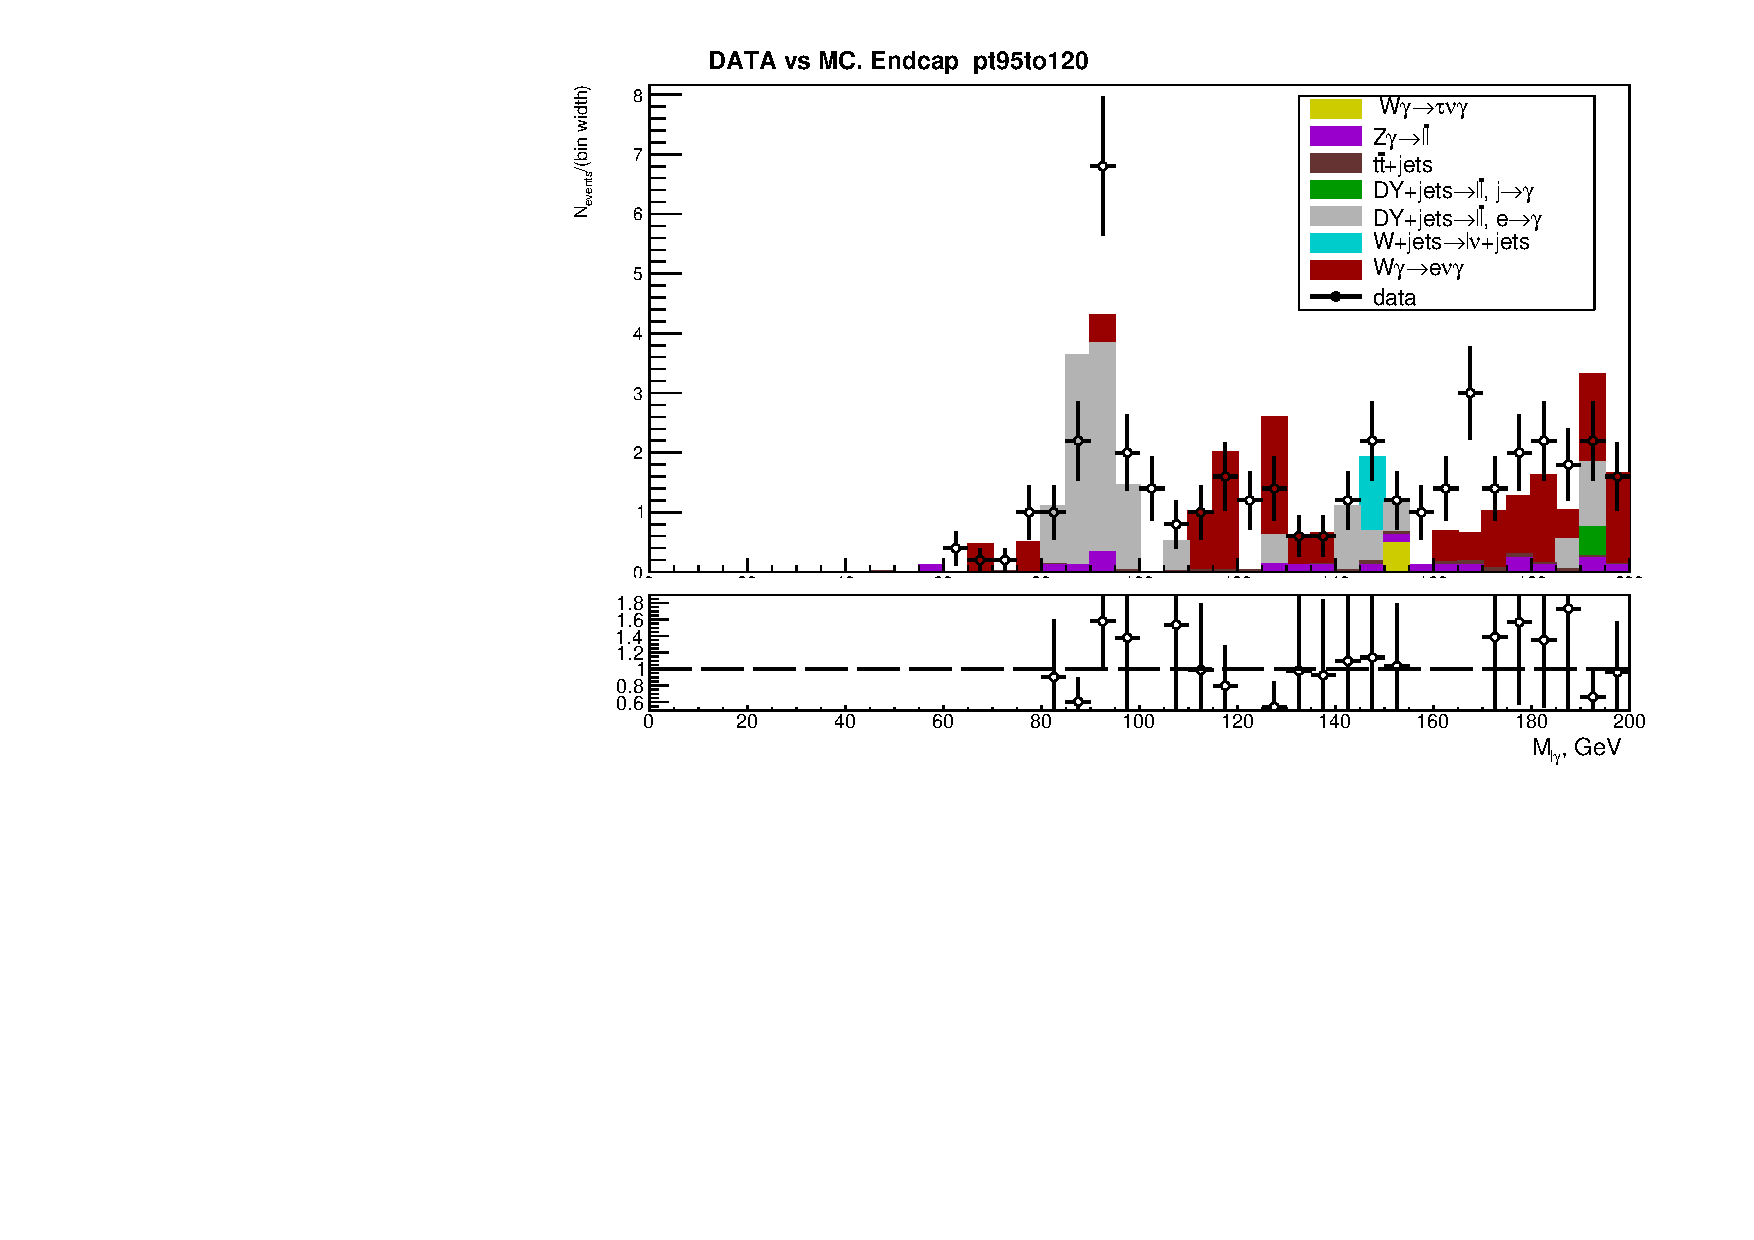
\includegraphics[width=0.40\textwidth]{../figs/figs_v11/ELECTRON_WGamma/PrepareYields/c_TotalDATAvsMC_Endcap__Mpholep1PRELIMINARY_FOR_E_TO_GAMMA_WITH_PSV_CUT_pt95to120_.pdf}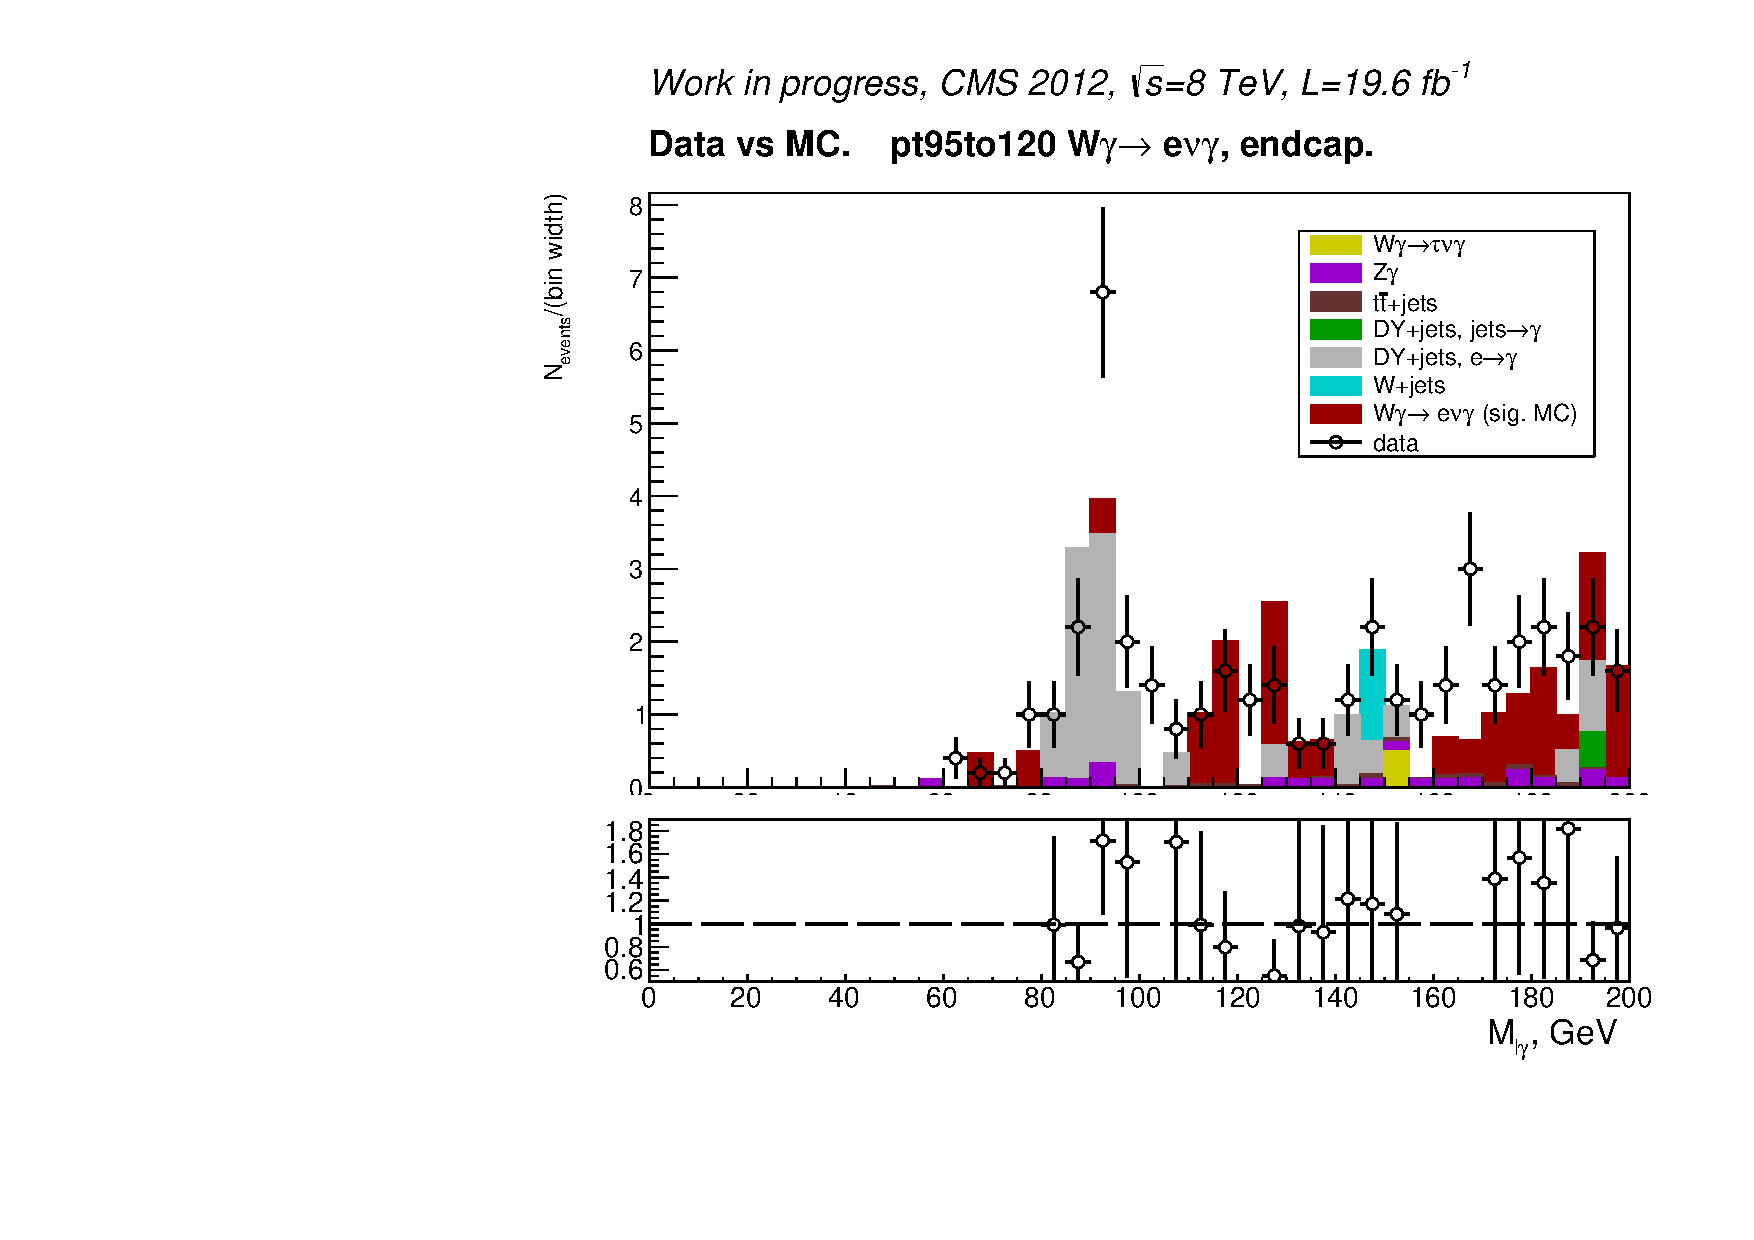
\includegraphics[width=0.40\textwidth]{../figs/figs_v11/ELECTRON_WGamma/PrepareYields/c_TotalDATAvsMC_Endcap__Mpholep1PRELIMINARY_FOR_E_TO_GAMMA_WITH_PSV_CUT_pt95to120__etogScale.pdf}\\
    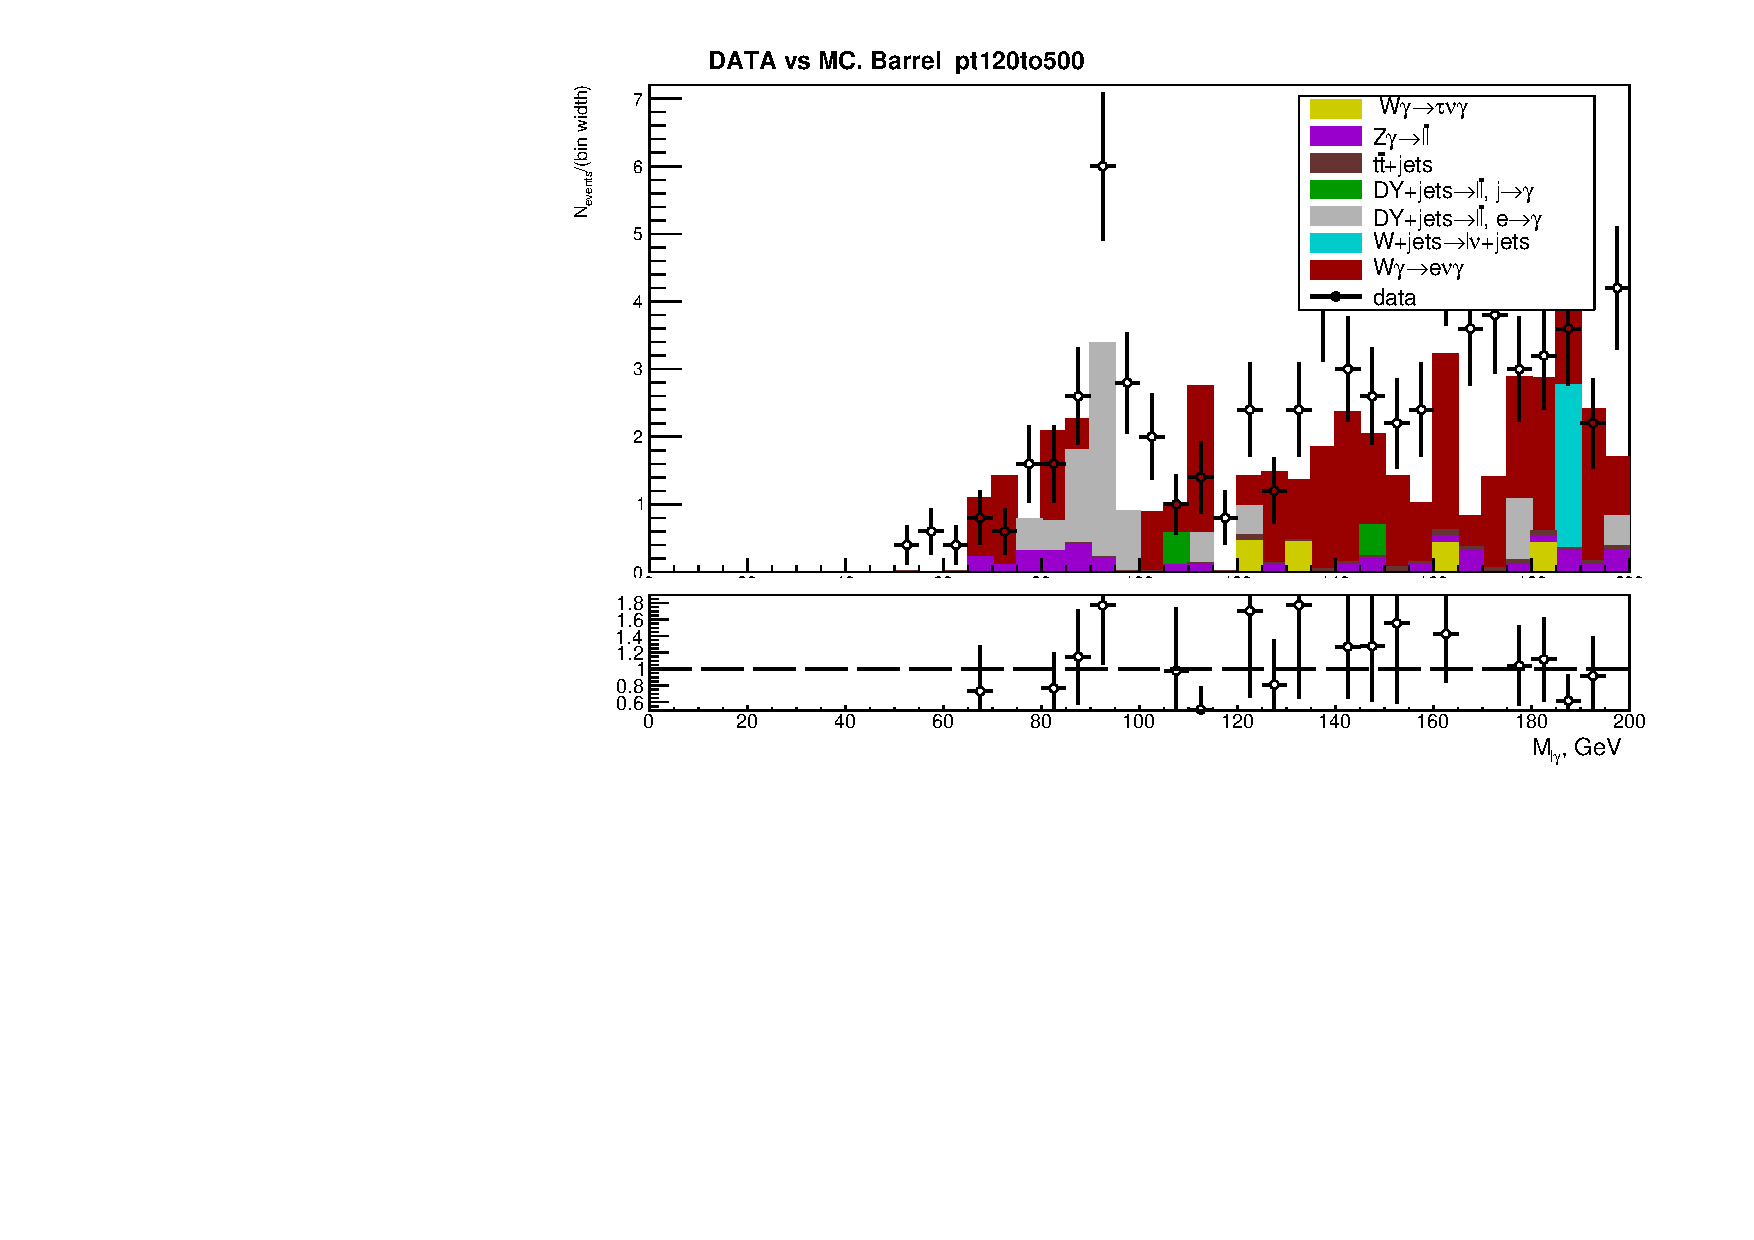
\includegraphics[width=0.40\textwidth]{../figs/figs_v11/ELECTRON_WGamma/PrepareYields/c_TotalDATAvsMC_Barrel__Mpholep1PRELIMINARY_FOR_E_TO_GAMMA_WITH_PSV_CUT_pt120to500_.pdf}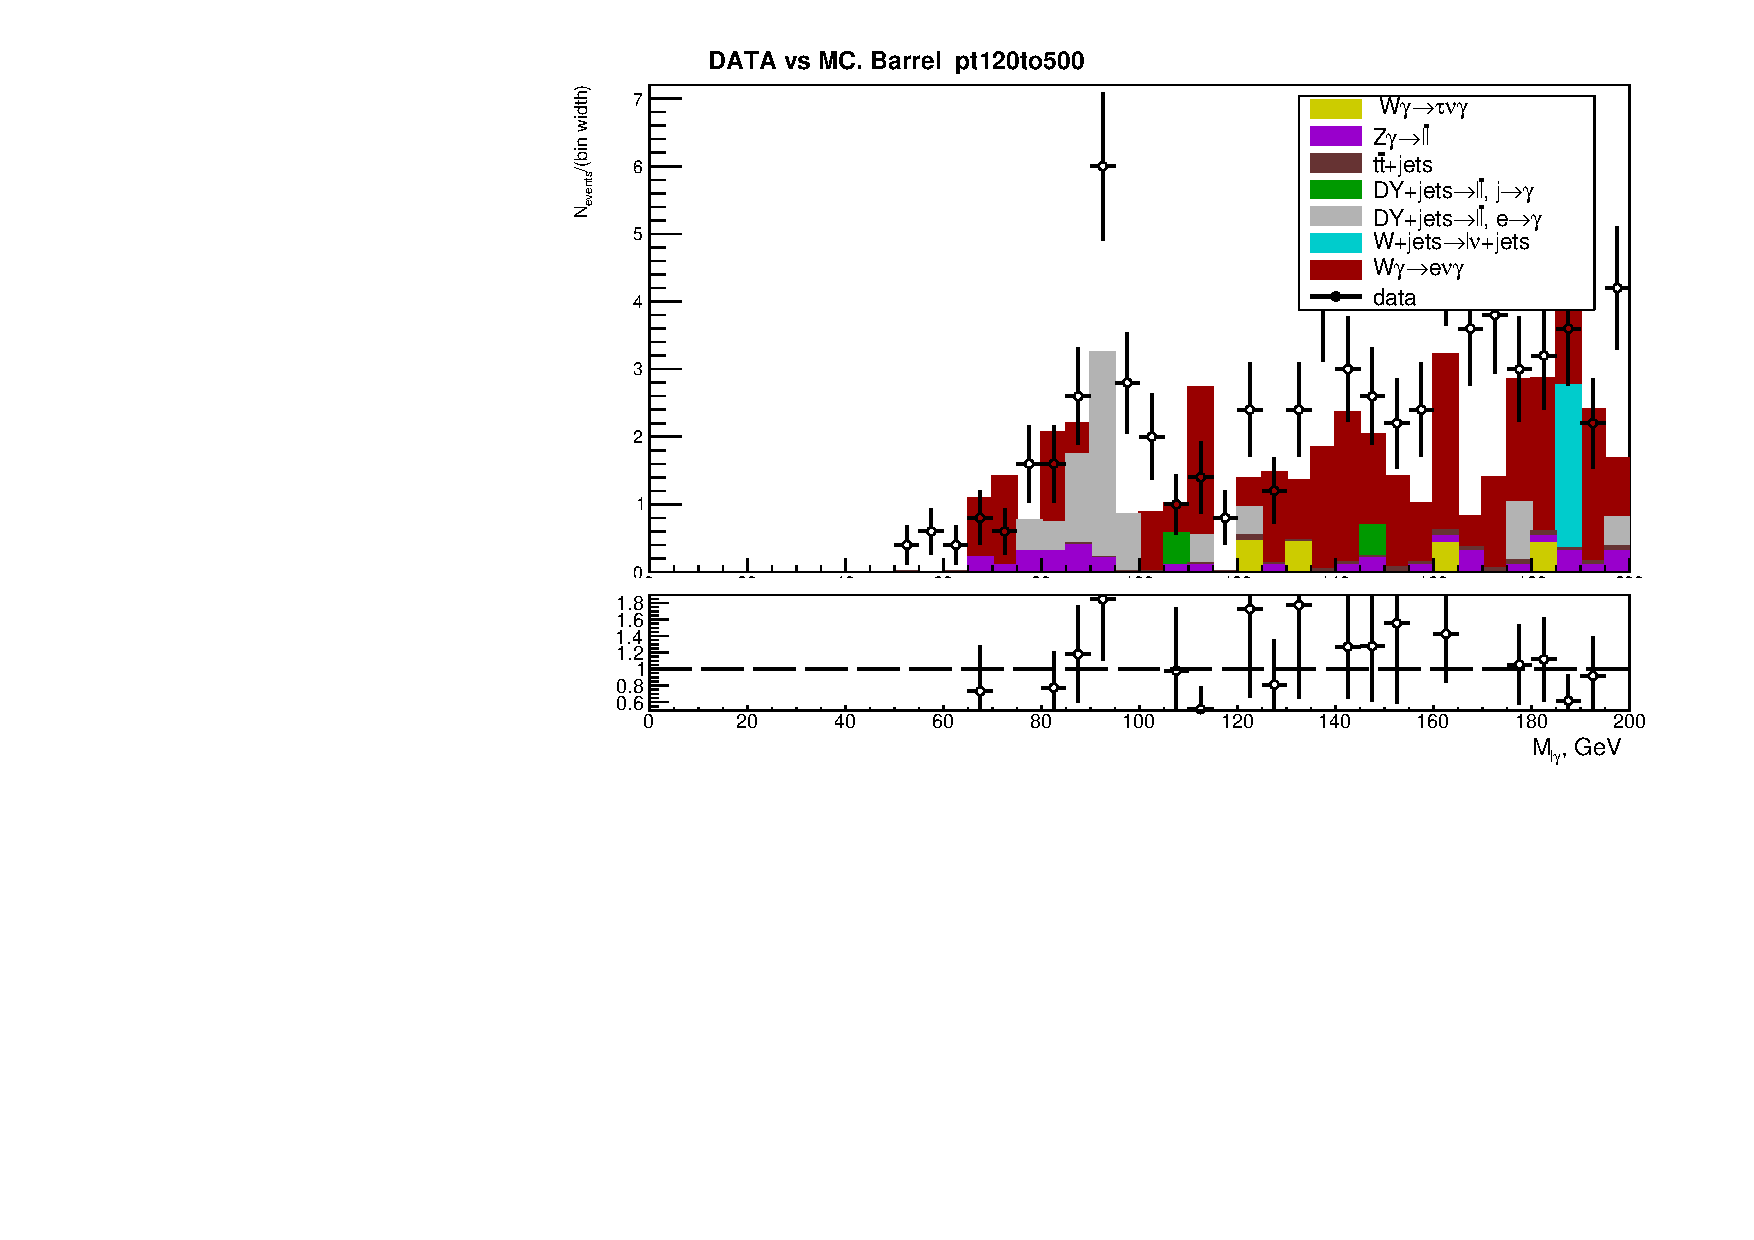
\includegraphics[width=0.40\textwidth]{../figs/figs_v11/ELECTRON_WGamma/PrepareYields/c_TotalDATAvsMC_Barrel__Mpholep1PRELIMINARY_FOR_E_TO_GAMMA_WITH_PSV_CUT_pt120to500__etogScale.pdf}\\
    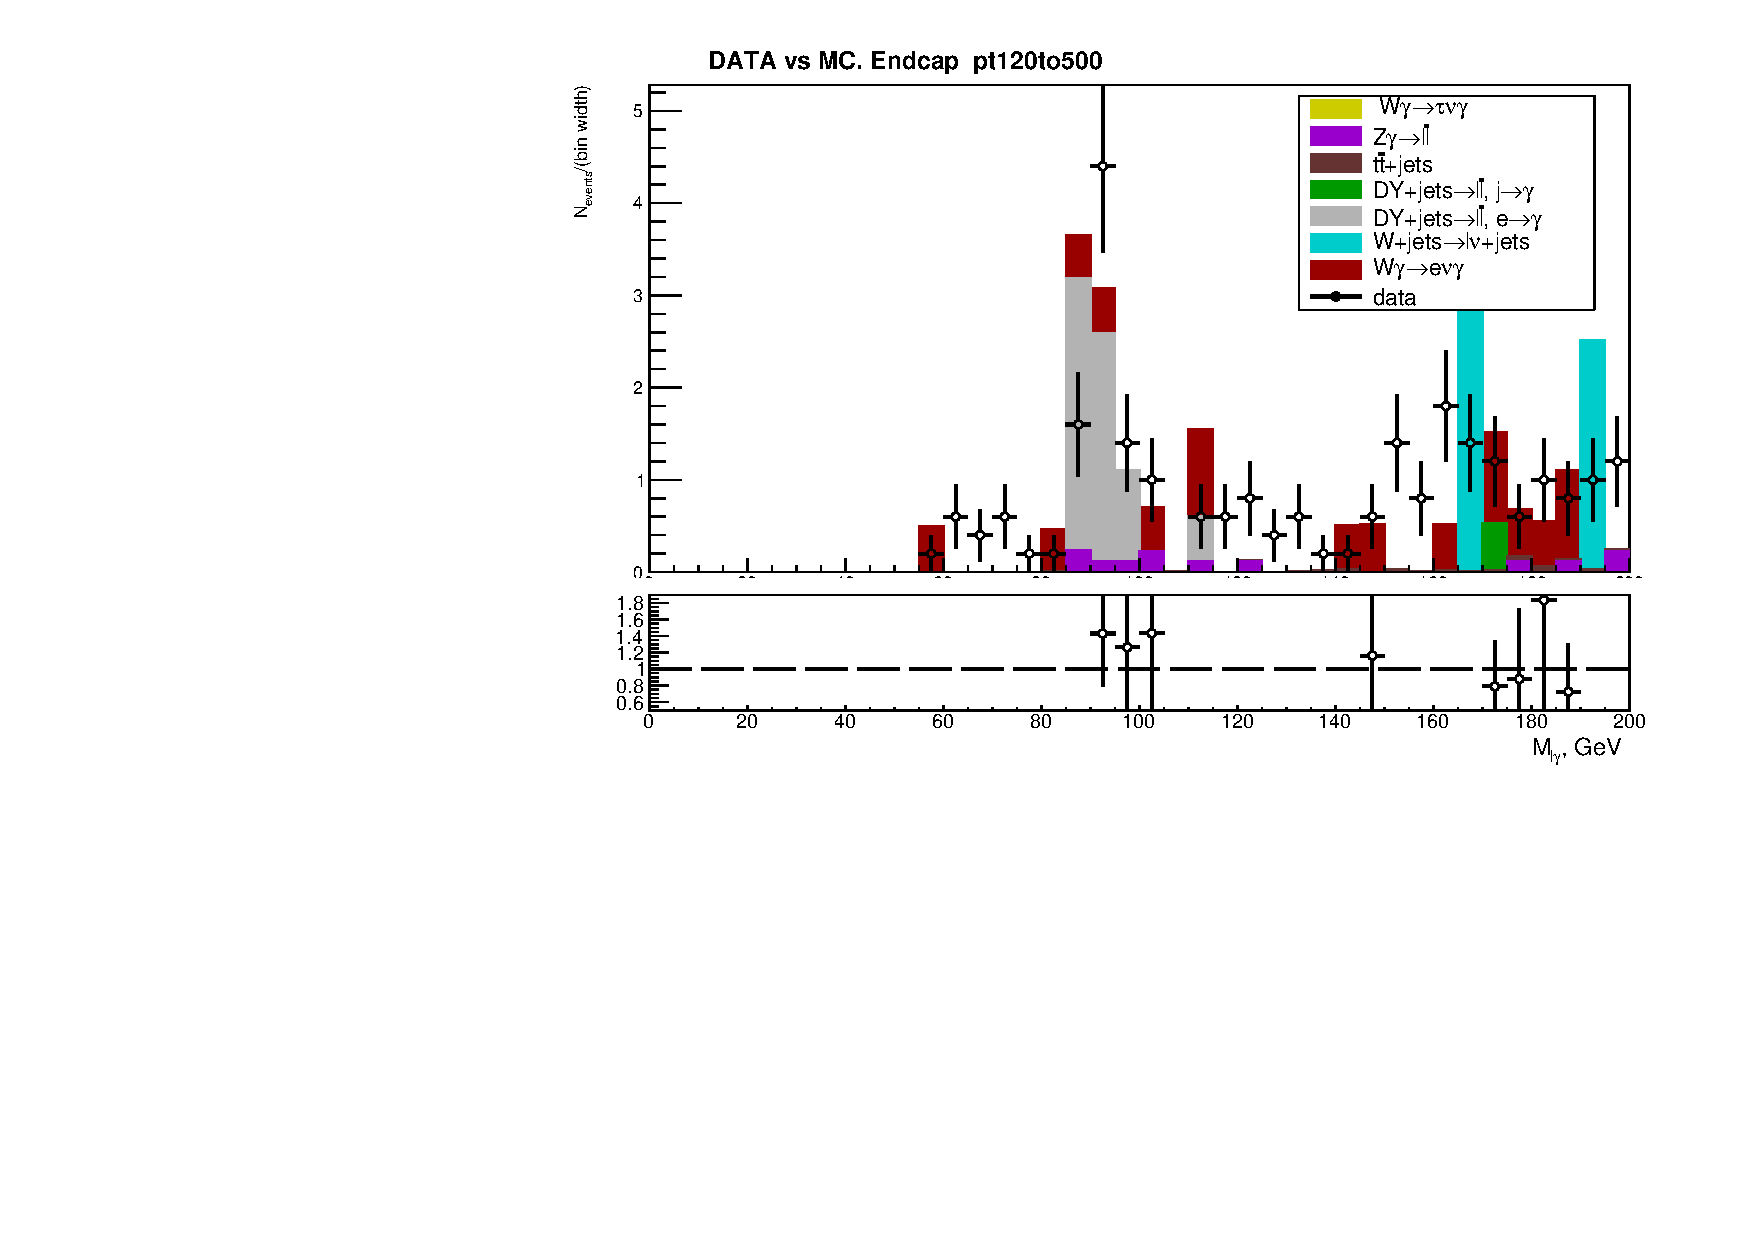
\includegraphics[width=0.40\textwidth]{../figs/figs_v11/ELECTRON_WGamma/PrepareYields/c_TotalDATAvsMC_Endcap__Mpholep1PRELIMINARY_FOR_E_TO_GAMMA_WITH_PSV_CUT_pt120to500_.pdf}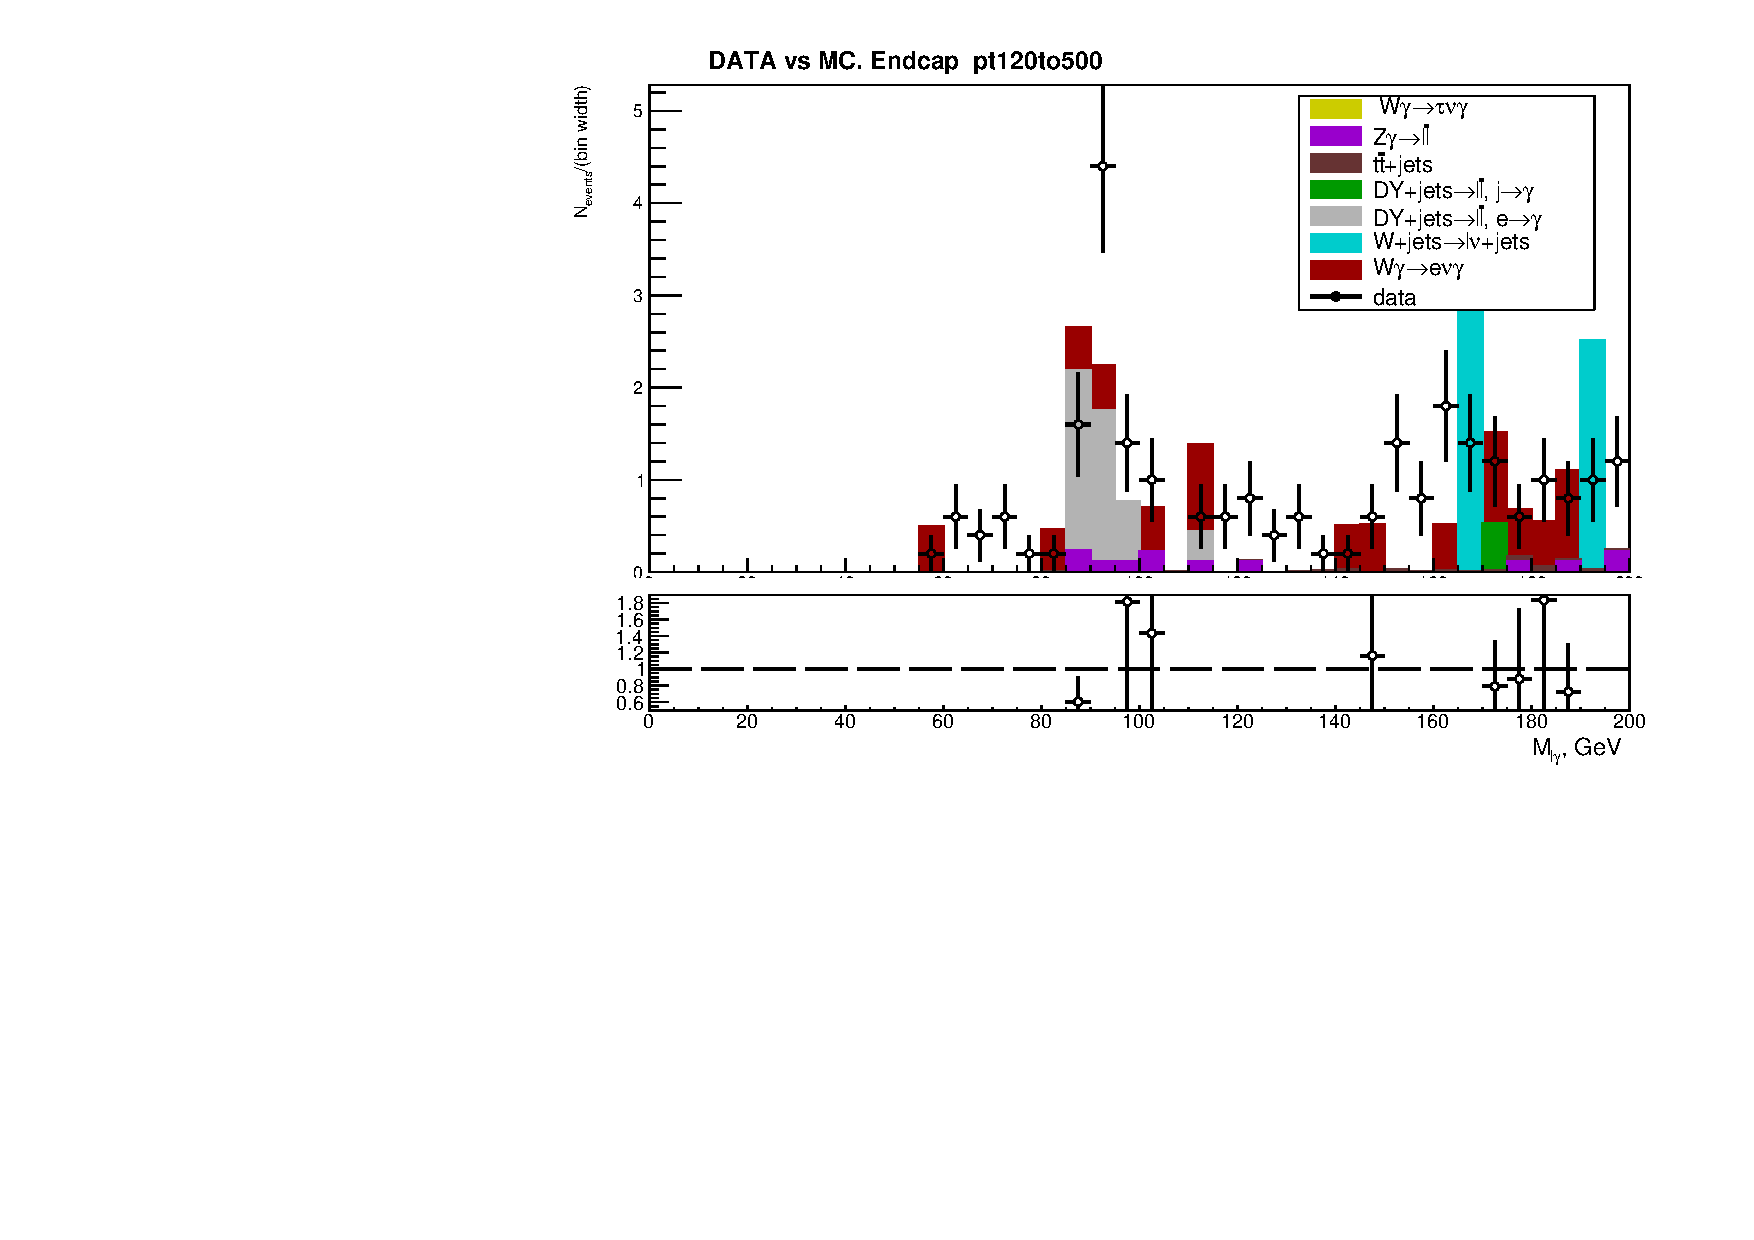
\includegraphics[width=0.40\textwidth]{../figs/figs_v11/ELECTRON_WGamma/PrepareYields/c_TotalDATAvsMC_Endcap__Mpholep1PRELIMINARY_FOR_E_TO_GAMMA_WITH_PSV_CUT_pt120to500__etogScale.pdf}\\
   \label{fig:Mpholep1DatavsMC_75to500}
  \caption{$M_{e,\gamma}$ distribution, data vs MC. Bins 95-120-500 GeV. Left: all MC samples are normalized to luminocity of data, PU weight adn SFs, right: DY$\rightarrow$jets(e$\rightarrow\gamma$) also normalized to e$\rightarrow\gamma$ data-driven estimates.}
  \end{center}
\end{figure}
